\documentclass[12pt, a4paper]{article}

%%%%%%%% PACKAGES - BEGIN %%%%%%%% 

\usepackage[utf8]{inputenc}
\usepackage[english, brazil]{babel}
\usepackage[inline]{enumitem}
\usepackage[a4paper,left=2.5cm,right=2.5cm,top=2.5cm,bottom=2.5cm]{geometry}
% \usepackage[subrefformat=parens,labelformat=parens]{subfig}
\usepackage{adjustbox}
\usepackage{amsfonts}
\usepackage{amsmath}
\usepackage{amsthm}
\usepackage{amssymb}
\usepackage{booktabs}
\usepackage{color}
\usepackage{float}
\usepackage{indentfirst}
\usepackage{graphicx, subfigure}
\usepackage{multirow}
\usepackage{multicol}
\usepackage{caption} 
\usepackage{setspace}
\usepackage{tabularx, booktabs}
\usepackage{tikz}
\usepackage{titling,lipsum}
\usepackage{hyperref}
\usepackage[num]{abntex2cite}
\usepackage[noend]{algpseudocode}
\usepackage{algorithm}
\usepackage{enumitem}
\usepackage{xfrac}
\usepackage{longtable}
\setlist{nolistsep}
\captionsetup[table]{skip=1pt}
\captionsetup[figure]{skip=0pt}
\citebrackets[] 
\usepackage{titlesec}
\titleformat*{\section}{\large\bfseries}
\titleformat*{\subsection}{\normalsize\bfseries}

%%%%%%%% PACKAGES - END %%%%%%%% 


%%%%%%%% COLOR DEFINITION - BEGIN %%%%%%%% 
\definecolor{c0}{HTML}{FFFFFF}
\definecolor{c1}{HTML}{FFC107}
\definecolor{c2}{HTML}{8BC34A}
\definecolor{c3}{HTML}{F44336}
\definecolor{c4}{HTML}{2196F3}
\definecolor{c5}{HTML}{9C27B0}

%%%%%%%% ALGORITHM REDEFINITION - END %%%%%%%%

\makeatletter
%%%%%%%% MATHEMATICS %%%%%%%%
\newcommand\floor[1]{\left\lfloor#1\right\rfloor}
\newcommand\ceil[1]{\lceil#1\rceil}

%%%%%%%% LINEAR MODEL %%%%%%%%
\newcommand{\pushright}[1]{\ifmeasuring@#1\else\omit\hfill$\displaystyle#1$\fi\ignorespaces}
\newcommand{\pushleft}[1]{\ifmeasuring@#1\else\omit$\displaystyle#1$\hfill\fi\ignorespaces}
\makeatother

%%%%%%%% TEMPLATE - BEGIN %%%%%%%%

\newcolumntype{Y}{>{\centering\arraybackslash}X}
\usetikzlibrary{arrows.meta}
\graphicspath{ {images/} }
\setlength{\parindent}{2em}
\singlespacing
\allowdisplaybreaks

%Evita quebra de palavras
%\tolerance=1
%\emergencystretch=\maxdimen
%\hyphenpenalty=10000
%\hbadness=10000

%emph bold and italic
\let\emph\relax
\DeclareTextFontCommand{\emph}{\bfseries\em}
\DeclareRobustCommand\iff{\Leftrightarrow}

% teorema 
\theoremstyle{plain}
\newtheorem{thm}{Teorema}[section]
\newtheorem{lem}[thm]{Lema}
\newtheorem{prop}[thm]{Proposição}
\newtheorem*{cor}{Corolário}
\theoremstyle{definition}
\newtheorem{defn}{Definição}[section]
\newtheorem{conj}{Conjectura}[section]
\newtheorem{exmp}{Exemplo}[section]
\theoremstyle{remark}
\newtheorem*{rem}{Remark}
\newtheorem*{note}{Nota}

\newcommand{\novo}[1]{\textcolor{blue}{#1}}
% \newcommand{\novo}[1]{#1}

\begin{document}

\selectlanguage{brazil}

\begin{center}
    {\normalsize\textbf{Instituto de Computação -  UNICAMP}}\\
    {\normalsize\textbf{Programação Linear Inteira - MO420}}\\
    {\normalsize\textbf{Primeiro Trabalho Prático}}
    \\ \bigskip
    {\normalsize Professor: Cid Carvalho de Souza}\\
    {\normalsize Aluno: Felipe de Carvalho Pereira}
\end{center}

\section{Introdução}

Este documento consiste em um relatório do projeto computacional desenvolvido na disciplina Programação Linear Inteira, ministrada no segundo semestre de 2019 pelo professor Cid C. de Souza. O trabalho objetivou o estudo e implementação do método dO subgradiente (MS) para uma relaxação lagrangiana do problema da Árvore Geradora com Número Mínimo de Ramificações (AGMR). Objetivou-se também o estudo e implementação de heurísticas para o MS, além de algoritmos de pré-processamento.

Introduzido por~\cite{Gargano2002}, o AGMR é definido da seguinte forma. A entrada é composta por um grafo $G = (V, E)$, conexo e não direcionado, onde $|V| = n$ e $|E| = m$. Além disso, denota-se por $T = (V^T, E^T)$ qualquer árvore geradora de $G$, de modo que um vértice $v \in V^T$ é considerado uma ramificação se seu grau é maior que $2$. Assim, estabelece-se como objetivo do AGMR a obtenção de uma árvore geradora de $G$ com quantidade mínima de ramificações. Em ~\cite{Gargano2002} também é mostrado que o problema pertence à classe $\mathcal{NP}$-difícil.

Uma formulação de Programação Linear Inteira (PLI) para AGMR é apresentada em~\cite{Carrabs2013} e considera os seguintes conjuntos de variáveis binárias:

\begin{itemize}[before=\vspace{\baselineskip},after=\vspace{\baselineskip}]

\item $x_e, \forall \, e \in E$: se a aresta $e$ pertence à solução, então $x_e = 1$, caso contrário, $x_e = 0$.
\item $y_v, \forall \, v \in V$: se o vértice $v$ é uma ramificação, então $y_v = 1$, caso contrário, $y_v = 0$.

\end{itemize}

Além disso, seja $S \subseteq V$, denota-se por $E(S)$ o conjunto de arestas que possuem ambos os extremos em $S$. Ademais, para todo $v \in V$, denotam-se por $A(v)$ e $\delta_v$, o conjunto de arestas incidentes em $v$ e o seu grau, respectivamente. A partir disso, a formulação segue:

{\abovedisplayskip=0pt
	\begin{align}
		\displaystyle \min z &= \; \sum_{v \in V} y_v \label{objective}\\
		\pushleft{\text{s.a.} \nonumber} & \\
		\displaystyle\sum_{e \in E} x_e &= \; n - 1 \label{tree_size}\\
		\displaystyle\sum_{e \in E(S)} x_e &\leq \; |S| - 1 &\forall \, S \subseteq V \label{no_cycle}\\
		\displaystyle\sum_{e \in A(v)} x_e - 2 &\leq \; \delta_v y_v &\forall \, v \in V \label{ramification}\\
		   y_v &\in \{0,1\} & \forall \, v \in V \label{var_y} \\
		   x_e &\in \{0,1\} & \forall \, e \in E \label{var_x}
	\end{align}
}

A função objetivo~\eqref{objective} minimiza o total de vértices que são ramificações. A restrição~\eqref{tree_size} estabelece que a solução contenha exatamente $n - 1$ arestas. Já a restrição~\eqref{no_cycle} impede a existência de ciclos. Perceba que estas duas restrições garantem que soluções viáveis sejam árvores geradoras. Ademais, a desigualdade~\eqref{ramification} determina que um vértice $v$ seja considerado uma ramificação se possuir mais do que duas arestas na árvore. Por fim, as restrições~\eqref{var_y} e~\eqref{var_x} definem o tipo binário das variáveis.

Observe que a restrição~\eqref{ramification} é satisfeita para qualquer vértice $v$, tal que $\delta_v \leq 2$. Logo, podemos definir o conjunto $V' = \{v \in V: \delta_v > 2\}$ e reescrever~\eqref{ramification} da maneira que segue.

{\abovedisplayskip=0pt
	\begin{align}
		\displaystyle\sum_{e \in A(v)} x_e - 2 &\leq \; \delta_v y_v &\forall \, v \in V' \label{ramification2}
	\end{align}
}

\section{Relaxação lagrangiana}

A relaxação lagrangiana proposta em~\cite{Carrabs2013} para o AGMR prevê a dualização das restrições~\eqref{ramification2}, de modo que o problema primal lagrangiano, com uso de multiplicadores $\lambda_v \geq 0 \; \forall v \in V'$ é descrito por $RL$, sujeito às restrições~\eqref{tree_size},~\eqref{no_cycle},~\eqref{var_y} e~\eqref{var_x}.

\begin{equation} \label{rl_original}
	(RL) \quad z(\lambda) = \min \sum_{v \in V'}y_v + \sum_{v \in V'}\lambda_v \left(\sum_{e \in A(v)}x_e -2 -\delta_v y_v \right) 
\end{equation}

Ao expandir os termos da equação, podemos reescrever $RL$ da maneira que segue, onde $RL_1$ está sujeito a \eqref{tree_size},~\eqref{no_cycle} e~\eqref{var_x}; e $RL_2$ sujeita-se a~\eqref{var_y}.

\begin{equation} \label{rl_mod}
	(RL) \quad z(\lambda) = -2 \sum_{v \in V'}\lambda_v + z_1(\lambda) + z_2(\lambda)
\end{equation}

\begin{equation} \label{rl_1}
	(RL_1) \quad z(\lambda) = \min \sum_{v \in V'}\lambda_v \sum_{e \in A(v)}x_e
\end{equation}

\begin{equation} \label{rl_2}
	(RL_2) \quad z(\lambda) = \min \sum_{v \in V'} y_v(1 - \delta_v \lambda_v)
\end{equation}

A partir da definição de $RL$, podemos definir o problema dual lagrangiano $DL$ associado a $RL$, que visa obter um conjunto de multiplicadores que maximize o problema primal.

\begin{equation} \label{dl}
	(DL) \quad \max_{\lambda \geq 0} z(\lambda) = \max_{\lambda \geq 0} -2 \sum_{v \in V'}\lambda_v + z_1(\lambda) + z_2(\lambda)
\end{equation}

Em ~\cite{Beasley1993}, encontramos que uma relaxação lagrangiana possui propriedade de integralidade quando uma solução ótima para o problema primal lagrangiano (para todos os multiplicadores possíveis), permanece inalterada ao substituir a restrição de integralidade das variáveis, isto é, $x\in\{0,1\}$, pela sua relaxação linear, ou seja, $0 \leq x \leq 1$. Ademais, quando isso acontece, temos que o melhor limitante dual obtido pela relaxação lagrangiana é igual àquele obtido pela relaxação linear do problema original.

É fácil perceber que a relaxação lagrangiana para o AGMR aqui apresentada possui propriedade de integralidade. Ao solucionar $RL_2$ via inspeção, ainda que as variáveis pudessem assumir valores reais, teríamos o mesmo critério de atribuição de valor. O problema $RL_1$, como veremos na seção seguinte, equivale ao problema chamado PAGM, cujo objetivo é encontrar uma árvore geradora mínima para um grafo dado. Para o PAGM é sabido que toda solução ótima também é ótima para sua relaxação linear, uma vez que todos os pontos extremos da relaxação linear do PAGM são inteiros.

Assim, concluímos que o melhor limitante dual que pode ser obtido através da relaxação lagrangiana do AGMR é igual ao limitante que seria obtido ao resolver a relaxação linear do problema. Para o AGMR, a vantagem da primeira em relação a segunda, consiste no fato de que a quantidade de restrições~\eqref{no_cycle} fazem parte da relaxação linear e são exponenciais no tamanho da entrada, tornando inviável a representação em memória computacional, à medida que a entrada cresce. Logo, resolver $DL$ equivale a resolver a relaxação linear do AGMR, mas sem a necessidade de representar explicitamente tais restrições. 

\section{Metodologia}

Nesta seção discutimos os métodos que foram utilizados neste trabalho para atacar o AGMR.

\subsection{Método do subgradiente}
\label{ms}
O método do subgradiente (MS) é uma estratégia conhecida para resolver problemas duais lagrangianos~\cite{Nemhauser1988}. Trata-se de um procedimento iterativo em que, a partir de um conjunto inicial de multiplicadores de Lagrange, novos multiplicadores são gerados, de modo que o problema dual lagrangiano seja solucionado por sucessiva trocas ajustadas destes multiplicadores~\cite{Beasley1993}. Essas mudanças geram uma sequência de movimentos no espaço de soluções do problema dual, ao longo da direção de seu subgradiente. Como $DL$ é uma função linear côncava por partes, podemos aplicar o MS para resolvê-la~\cite{Carrabs2013}.

A implementação do MS neste trabalho foi realizada de acordo com a descrição do algoritmo em \cite{Carrabs2013}. As rodadas são denotadas por $k$ e, na rodada $k = 0$, configuram-se os valores iniciais dos multiplicadores da seguinte maneira:

\begin{center}
	$\lambda_v = \max\limits_{u \in V'} \left\{\dfrac{1}{\delta_v}\right\}, \forall \; v \in V'$.
\end{center}

O segundo passo consiste em resolver $RL$ para os multiplicadores definidos, obtendo a solução $(x(\lambda^{(k)}), y(\lambda^{(k)}))$ e o seu respectivo valor $z(\lambda^{(k)})$. Os algoritmos usados para solucionar $RL$ serão discutidos mais à frente. Em seguida, obtém-se o vetor subgradiente, tal que a $v$-ésima componente do vetor pode ser calculada por:

\begin{center}
	$g_v^{(k)} = \displaystyle\sum_{e \in A(v)} x_e (\lambda^{(k)}) - 2 - \delta_v y_v(\lambda^{(k)})$.
\end{center}

Seja $z_{up}$ o melhor limitante superior obtido para o problem original, então o quarto passo corresponde ao cálculo do tamanho do passo $t_k$ a partir da expressão:

\begin{center}
	$t_k = \epsilon_k \dfrac{z_{up} - z(\lambda^{(k)})}{\lVert g^{(k)}\rVert^2}$
\end{center}

No quinto passo, os multiplicadores são atualizados utilizando o seguinte critério:

\begin{center}
	$\lambda_v^{(k+1)} =
	\begin{cases}
	0 & \text{se } \lambda_v^{(k)} + t_k g_v^{(k)} < 0 \\
	\lambda_v^{(k)} + t_k g_v^{(k)} & \text{se } 0 \leq \lambda_v^{(k)} + t_k g_v^{(k)} \leq \dfrac{1}{\delta_v}\\
	\dfrac{1}{\delta_v} & \text{caso contrário}
	\end{cases}$
\end{center}

Finalmente, no sexto passo, avançamos para a iteração seguinte fazendo $k = k + 1$. Daí, o algoritmo retorna ao passo $2$. A finalização do algoritmo pode ser definida por um número limite de iterações ou por tempo limite de execução.

No segundo passo do algoritmo, dois diferentes algoritmos são utilizados para resolver $RL_1$ e $RL_2$, respectivamente. Para obter a solução ótima do $RL_2$, basta realizar um procedimento de inspeção sobre as variáveis $y_v$, isto é, faz-se $y_v = 1$, se $(1 - \delta_v \lambda_v) < 0$ ou $y_v = 0$, caso contrário. É fácil perceber que, no pior caso, a complexidade da inspeção é $\theta(V)$.

Ademais, o problema $RL_1$ corresponde ao PAGM, onde o peso de cada aresta $\{u, v\}$ é definido por $\lambda_u + \lambda_v$. Existem dois algoritmos gulosos e polinomiais bem conhecidos para o PAGM, são eles os algoritmos de Prim e o de Kruskal. O primeiro tem complexidade conhecida de $O(|E| + |V|\log|V|)$ no pior caso, com uso lista de adjacência e \textit{heap} de Fibonacci. Já o algoritmo de Kruskal tem complexidade $O(|E|\log|V|)$ no pior caso~\cite{Cormen2009}.

Observe que, para grafos densos, ou seja, quando $|E| = O(|V|^2)$, o algoritmo de Prim é preferível, pois no pior caso teria complexidade $O(|V|^2 + |V|\log|V|)$, já o segundo teria complexidade $O(|V|^2\log|V|)$. Quando grafos esparsos são fornecidos na entrada, ou seja, $|E| = O(|V|)$, opta-se pelo uso do algoritmo de Kruskal, pois no pior caso, tem-se complexidade $O(|V|\log|V|)$, já para o primeiro, tem-se $O(|V| + |V|\log|V|)$.

Nas implementações adotadas neste trabalho, adotou-se o algoritmo de Kruskal para resolução do $RL_1$, uma vez que, para os experimentos computacionais previstos no projeto, as instâncias contém grafos esparsos. 

Durante a execução do MS, existem duas maneiras de verificar a obtenção de otimalidade. A primeira é trivial e ocorre quando o melhor limitante dual encontrado igualou-se ao melhor limitante primal. Logo, a solução que gerou o melhor limitante primal é ótima. Note que como o AGMR tem valor de solução inteiro, então pode-se considerar o teto do limitante dual obtido via MS, afim de comprovar otimalidade. A segunda maneira consiste em verificar se a solução que gerou o limitante dual é ótima para o AGMR.

Segundo~\cite{Beasley1993}, supondo que os multiplicadores de Lagrange são maiores ou iguais a $0$, então uma solução do problema primal lagrangiano é ótima para o problema original se a solução é factível para o problema original e se a restrição dualizada é satisfeita na igualdade quando o multiplicador correspondente é estritamente positivo.

Para o MS aplicado ao AGMR, temos, a cada iteração, uma solução $X = (x_e, y_v)$ do $RL$. Observe que as variáveis $x_e$ contém a solução ótima para o $RL_1$, e portanto, não possui ciclos, atendendo à restrição~\eqref{no_cycle}, e contém exatamente $n - 1$ arestas, atendendo à restrição~\eqref{tree_size}. Além disso, $X$ é inteira e atende às restrições~\eqref{var_x} e~\eqref{var_y}. Logo, para verificar a factibilidade de $X$ para o problema original, basta verificar se as variáveis $y_v$ atendem à restrição~\eqref{ramification2}.

Uma vez que $X$ é factível para o problema primal, verificamos se a restrição~\eqref{ramification2} é satisfeita na igualdade sempre que o $\lambda$ correspondente é positivo. Se sim, então $X$ é ótima para o problema original. Neste trabalho ambas as técnicas de verificação de otimalidade foram implementadas e são executadas em todas as iterações do MS.

\subsection{Heurísticas para o MS}

Foram estudadas e implementadas duas heurísticas para utilização durante o MS, chamadas IMP1 e IMP2. Ambas são propostas em~\cite{Marin2015} e são iniciadas a partir de uma solução factível do AGMR, isto é, uma árvore geradora qualquer.

A heurística IMP1 itera sobre o conjunto de arestas que estão fora da árvore. Se uma aresta $e = (v, u)$, tal que $\delta_v \neq 2$ e $\delta_u \neq 2$, é encontrada, então verifica-se a existência de uma aresta $e'$ pertencente ao caminho de $v$ para $u$ na árvore, tal que uma das extremidades de $e'$ tem grau igual a $3$, excetuando $v$ e $u$. Se $e'$, existe então tal aresta é removida da árvore e a aresta $e$ é adicionada. Note que, se $e$ e $e'$ forem devidamente encontradas, tal procedimento produz uma nova árvore geradora com pelo menos uma ramificação a menos. O algoritmo para quando todas as arestas que estavam inicialmente fora da árvore foram testadas.

A complexidade de IMP1 no pior caso é $O(|E||V|)$, onde o custo para checar todas as arestas fora da árvore é $O(|E|)$ e o custo para obter o caminho entre dois vértices na árvore é $O(|V|)$. Note que para grafos esparsos, podemos ter pior caso em $O(|V|^2)$.

O algoritmo IMP2 também itera sobre o conjunto de arestas que estão fora da árvore. Se uma aresta $e = (v, u)$, tal que $\delta_v \neq 2$, é encontrada, então considera-se a aresta $e' = (u, x)$ existente no caminho de $v$ para $u$ na árvore, com $x \neq v$. Se $\delta_x = 3$, então a aresta $e'$ é removida da árvore e a aresta $e$ é adicionada. Observe que, se $e$ e $e'$ forem devidamente encontradas, o procedimento produz uma nova árvore geradora com uma ramificação a menos. A heurística é finalizada quando todas as arestas que estavam inicialmente fora da árvore foram testadas. A análise de complexidade do IMP2 é análoga a do IMP1, com mesmo custo para o pior caso.

Neste trabalho, a cada iteração do MS, ambas as heurísticas são acionadas após a resolução de $RL$ e recebem como entrada a solução de $RL_1$. Ao serem iniciadas, IMP1 e IMP2 são executadas alternadamente até que, em algum momento, nenhuma das duas heurísticas produzam melhoria o valor da solução.

\subsection{Pré-processamento}

Neste trabalho foi implementada uma técnica de pré-processamento proposta em~\cite{Marin2015} para o AGMR. Tal técnica consiste em duas fases. Na primeira, constrói-se uma arborescência para o grafo original através de uma busca em profundidade. Note que uma arborescência de um grafo é um subgrafo direcionado no qual existe um vértice raiz $v$, e, para qualquer outro vértice $u$, só existe um único caminho direcionado de $v$ para $u$. A partir da arborescência, verifica-se quais arestas do grafo são pontes. Uma aresta é denominada ponte se sua deleção resulta no aumento do número de componentes do grafo.

Observe que a entrada do AGMR é composta por um grafo conexo. Isso significa que as pontes estão presentes em todas as soluções ótimas do problema. Ademais, se um vértice $v$ possui $3$ pontes incidentes, ou, se $v$ possui $2$ pontes incidentes e $\delta_v \geq 3$, então $v$ é uma ramificação em todas as soluções viáveis do problema. Neste trabalho, essa técnica de pré-processamento foi utilizada como rotina a ser executada antes do MS. Uma vez identificadas as pontes e as ramificações, as variáveis correspondentes à estes são fixadas no valor $1$.

A vantagem de fixar $x_e = 1$ para alguma ponte $e \in E$ consiste no fato de que podemos inserir $e$ previamente em todas as soluções do $RL_1$. Como fazemos uso do algoritmo de Kruskal para resolver tal problema, então as arestas fixadas podem ser inseridas diretamente na árvore geradora, antes da execução do algoritmo e sem a necessidade de verificar se os extremos de $e$ pertencem à conjuntos disjuntos. O resultado disso é uma amortização no custo de resolver $RL_1$, dada em função do número de pontes encontradas no pré-processamento.

Ademais, fixar $y_v = 1$ para alguma ramificação $v$ identificada no pré-processamento, nos permite que a restrição em~\eqref{ramification2} correspondente à $y_v$ não seja dualizada. Isto equivale a definir o conjunto $V'' = \{v \in V': v \text{ é uma ramificação}\}$ e rescrever~\eqref{ramification2} da seguinte forma:

{\abovedisplayskip=0pt
	\begin{align}
		\displaystyle\sum_{e \in A(v)} x_e - 2 &\leq \; \delta_v y_v &\forall \, v \in V' \setminus V'' \label{ramification3}
	\end{align}
}

Assim, ajustamos o problema $RL$, incluindo o valor da variável de cada uma das ramificações, isto é, $|V''|$:

\begin{equation} \label{rl_mod_pre}
	(RL) \quad z(\lambda) = |V''| -2 \sum_{v \in V' \setminus V''}\lambda_v + z_1(\lambda) + z_2(\lambda)
\end{equation}

\section{Experimentos}

Nesta seção, apresentamos como os experimentos computacionais foram conduzidos neste trabalho e quais resultados foram obtidos.
 
\subsection{Configurações}

Um conjunto de $400$ instâncias com quantidades de vértices entre $20$ e $500$ foram utilizadas para a condução de experimentos neste trabalho. Tais instâncias também foram empregadas em~\cite{Carrabs2013}. Além disso, estabelecemos $7$ diferentes configurações de execuções, a saber:

\begin{itemize}[before=\vspace{\baselineskip},after=\vspace{\baselineskip}]
\item A: ;
\item B: ;
\item C: ;
\item D: ;
\item E: ;
\item F: ;
\item G: ;
\end{itemize}

Cada configuração foi executada uma vez para cada uma das instâncias, totalizando $1600$ casos de teste. Em todas as configurações, o parâmetro $\epsilon$ foi fixado em $0,01$ para todas as iterações do MS. Em experimentos preliminares com uma pequena amostra de instâncias, tal valor de $\epsilon$ gerou resultados melhores que os demais valores testados. Ademais, nas configurações SG e SG-P, em que não há o uso de heurísticas, os limitantes superiores utilizados pelo MS são obtidos pela solução do $RL_1$ a cada iteração.

Para cada caso de teste, estabeleceu-se o limite de tempo de execução de $10$ segundos, incluídos os tempos de pré-processamento e heurísticas para as configurações que contam com tais rotinas. Entretanto, configuramos o MS para ser finalizado quando algum dos dois critérios de otimalidade, discutidos na seção~\ref{ms}, é atingido. Os casos de teste foram executados sequencialmente em uma mesma máquina. Tal máquina contém 8GB de memória RAM e um processador Intel Core i7-7500U com \textit{clock} de 2.70GHz.

\subsection{Resultados}

Os resultados dos experimentos estão dispostos nas tabelas~\ref{t1},~\ref{t2},~\ref{t3},e~\ref{t4}, referentes às configurações SG, SG-P, SG-H e SG-P-H, respectivamente. As colunas de cada tabela correspondem às seguintes informações:

\begin{itemize}[before=\vspace{\baselineskip},after=\vspace{\baselineskip}]
\item \textbf{Instância}: nome da instância;
\item \textbf{LB}: melhor limitante inferior obtido;
\item \textbf{ILB}: iteração em que o melhor limitante inferior foi obtido;
\item \textbf{TLB}: tempo em que o melhor limitante inferior foi obtido (em segundos);
\item \textbf{UB}: melhor limitante superior obtido;
\item \textbf{IUB}: iteração em que o melhor limitante superior foi obtido;
\item \textbf{TUB}: tempo em que o melhor limitante superior foi obtido (em segundos);
\item \textbf{GAP}: \textit{gap} de otimalidade entre os melhores limitantes;
\item \textbf{ITER}: número total de iterações realizadas;
\item \textbf{TIME}: tempo total da execução (em segundos);
\item \textbf{OPTG}: otimalidade verificada por \textit{gap} ($0$ para não e $1$ para sim);
\item \textbf{OPTS}: otimalidade verificada por solução primal lagrangiana ($0$ para não e $1$ para sim).
\end{itemize}

Observando as tabelas mencionadas, fica claro que, em geral, para uma mesma instância, a quantidade de iterações do MS realizada pelas configurações SG e SG-P é bastante superior àquelas realizadas por SG-H e SG-P-H. Esse comportamento era esperado e se deve ao fato de que há um \textit{overhead} causado pelo uso das heurísticas a cada iteração. Note que SG-P contém a rotina de pré-processamento, mas ela só é realizada uma única vez antes da execução do MS, ocasionando um \textit{overhead} mínimo. Quanto ao tempo gasto pelas configurações, temos que, excetuando as execuções que alcançaram otimalidade, todas as demais atingiram o limite de tempo estabelecido de $10$ segundos.

Para analisar a qualidade dos limitantes inferiores, utilizaremos o critério de arredondamento para cima dos limitantes inferiores, uma vez que todo valor de solução do AGMR é inteiro. Assim, temos que, apenas para $6$ instâncias, SG-H obteve melhores limitantes inferiores que SG. Por outro lado, SG obteve melhores limitantes que SG-H para $231$ instâncias. Além disso, para a ampla maioria das execuções, o melhor limitante inferior foi obtido na iteração $k = 1$. Isso mostra que a utilização de heurísticas não surtiu efeito positivo na melhoria dos limitantes inferiores.

Quanto ao uso de pré-processamento, verificou-se que para $375$ instâncias, SG-P obteve melhores limitantes inferiores que SG. Na média, a diferença entre os limitantes gerados por SG-P e SG-P é igual a $17.18$, de modo que a maior discrepância foi de $70$. Comparando SG-P e SG-P-H, verificamos que, SG-P gerou, para $170$ instâncias, melhores limitantes inferiores que SG-P-H. Isso corrobora a observação anterior de que as heurísticas propostas contribuíram negativamente para a melhoria dos limitantes inferiores. Entretanto, a diferença máxima encontrada entre os limitantes produzidos por SG-P e SG-P-H foi de $2$.

Agora, partiremos para uma análise da qualidade dos limitantes superiores. Verificamos que a configuração SG-H obteve melhores limitantes superiores para $375$ instâncias, em relação a SG. Na média, a diferença entre os limitantes gerados por SG-H e SG foi de $6.90$, enquanto que a maior discrepância registrada foi de $23$. Para apenas uma instância SG foi capaz de gerar um limitante superior melhor que SG-H.

Ademais, observamos que a configuração SG-P gerou melhores limitantes superiores que SG-H apenas para $26$ instâncias, tendo sido superada em outras $320$ instâncias. Entretanto, verificamos que a configuração SG-P-H superou SG-H em $265$ instâncias, de modo que, apenas para $24$ instâncias, SG-H obteve melhores limitantes superiores que SG-P-H. Isso mostra que para a obtenção de melhores limitantes superiores, o uso combinado de heurísticas e pré-processamento apresentou desempenho superior às demais configurações.

Analisaremos agora as instâncias para as quais conseguiu-se obter uma solução ótima. A tabela~\ref{opt} exibe
as 12 instâncias para as quais a otimalidade foi verificada por checagem de \textit{gap}, além dos seus respectivos valores ótimos. Nenhuma instância teve otimalidade verificada via solução primal lagrangiana. Através da tabela, concluímos também que as configurações SG, SG-P, SG-H e SG-PH geraram soluções ótimas para, respectivamente, $1$, $8$, $2$ e $6$ instâncias. 

% Please add the following required packages to your document preamble:
% \usepackage{booktabs}
\begin{table}[H]
\centering
\caption{Otimalidade de instâncias}
\label{opt}
\begin{tabular}{@{}lccccc@{}}
\toprule
\multicolumn{1}{c}{Instância} & SG                    & SG-P                  & SG-H                  & SG-P-H                & z* \\ \midrule
Spd\_RF2\_20\_27\_227         &                       & \checkmark &                       &                       & 2  \\
Spd\_RF2\_20\_27\_235         &                       & \checkmark &                       & \checkmark & 3  \\
Spd\_RF2\_20\_27\_243         &                       & \checkmark &                       & \checkmark & 4  \\
Spd\_RF2\_20\_34\_259         &                       & \checkmark &                       &                       & 1  \\
Spd\_RF2\_20\_42\_291         & \checkmark & \checkmark &                       &                       & 1  \\
Spd\_RF2\_20\_42\_299         &                       & \checkmark &                       &                       & 0  \\
Spd\_RF2\_20\_49\_331         &                       &                       &                       & \checkmark & 0  \\
Spd\_RF2\_20\_49\_355         &                       &                       & \checkmark &                       & 0  \\
Spd\_RF2\_20\_49\_363         &                       &                       &                       & \checkmark & 0  \\
Spd\_RF2\_40\_50\_619         &                       & \checkmark &                       &                       & 7  \\
Spd\_RF2\_20\_57\_403         &                       &                       & \checkmark & \checkmark & 0  \\
Spd\_RF2\_60\_71\_1043        &                       & \checkmark &                       & \checkmark & 15 \\ \bottomrule
\end{tabular}
\end{table}

Por fim, analisaremos a variação dos limitantes inferior e superior, além do tamanho do passo, na execução da configuração SG-P com a instância \textit{Spd\_RF2\_100\_159\_1939}. Tais dados estão apresentados na figura~\ref{fig:graphic}, onde denotam-se:

\begin{itemize}[before=\vspace{\baselineskip},after=\vspace{\baselineskip}]
\item \textbf{BLB}: melhor limitante inferior obtido;
\item \textbf{CLB}: limitante inferior corrente, obtido na iteração $k$;
\item \textbf{BUB}: melhor limitante superior obtido;
\item \textbf{CUB}: limitante superior corrente, obtido na iteração $k$;
\item \textbf{t\_k}: tamanho do passo na iteração $k$.
\end{itemize}

\begin{figure}[H]
\centering     %%% not \center
\caption{Variação de limitantes e tamanho de passo durante execução do MS} \label{fig:graphic} 
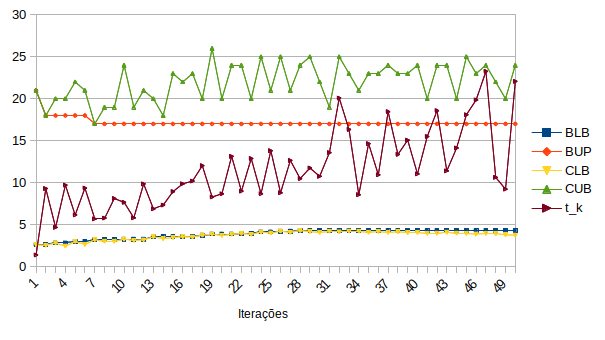
\includegraphics[height=0.5\textwidth]{pics/graphic.png}
\end{figure}

O tamanho do passo, $t_k$, pode ser obtido ao multiplicar $10^{-3}$ pelo valor representado no gráfico na iteração $k$. Ademais, por razões de legibilidade, omitimos a iteração $k = 0$, na qual, BLB = CLB = $-165$, BUP = CUB = $21$ e $t_k = 13 10^{-3}$. Também omitimos as iterações a partir de $k \geq 50$, pois os limitantes permanecem inalterados.

O valor de CLB negativo na iteração $0$ pode ser explicado pela configuração inicial dos multiplicadores. Multiplicadores demasiadamente altos, contribuem para aumento do primeiro termo de $z(\lambda)$, $-2 \sum_{v \in V'} \lambda_v$, que é negativo, resultando em um possível limitante inferior muito negativo.

A variação dos limitantes corresponde a um comportamento esperado para o MS, onde podemos perceber uma diminuição gradual do \textit{gap} à medida que as iterações avançam. Observe que até a iteração $28$, a cada $5$ iterações, houve mudança em pelo menos um dos dois melhores limitantes. Nesse intervalo, tanto o valor de $t_k$, quanto a sua variação entre as iterações é menor do que aquilo que temos a partir da iteração $30$.

Isso sugere que, enquanto havia melhoria frequente no \textit{gap}, o tamanho do passo permaneceu menor e com mudanças menos abruptas, evitando que movimentos grandes fossem feitos no subgradiente. Entretanto, uma vez que o \textit{gap} passou a não apresentar melhorias, tamanhos de passos mais largos foram adotados, além de variações mais discrepantes entre as iterações, ocasionando movimentos maiores na busca por novos limitantes. Notemos ainda que, na configuração SG-P, CUB é influenciado diretamente pelo $t_k$, uma vez que este contribui na determinação dos novos multiplicadores, os quais são utilizados para calcular os pesos das arestas no $RL_1$. Tal influência pode ser observada na figura~\ref{fig:graphic}.

\section{Conclusão}

Todas as atividades previstas para este trabalho foram devidamente realizadas. Dentre as principais, podemos mencionar o estudo e implementação do MS, além da análise e implementação de heurísticas e técnicas de pré-processamento para o AGMR.

Além disso, um conjunto de experimentos foi conduzido e, a partir dos resultados obtidos, constatamos que a configuração SG-P obteve melhor desempenho quanto à qualidade dos limitantes inferiores gerados. Diante dos dados apresentados, associamos o bom desempenho deste algoritmo ao uso das técnicas de pré-processamento propostas. Também verificamos que a configuração SG-P-H foi capaz de produzir melhores limitantes superiores em relação às demais configurações. O uso das heurísticas propostas revelou uma melhoria na obtenção de tais limitantes. Essa melhoria foi potencializada com o uso combinado das heurísticas e do pré-processamento.

De um modo geral, consideramos que os resultados produzidos eram esperados. Entretanto, observou-se que o uso de heurísticas surtiu um efeito negativo quanto a qualidade dos limitantes inferiores. A priori, existe a possibilidade de que isso se deva à quantidade reduzida de iterações quanto ao uso de heurísticas. Todavia, verificou-se que para a maioria das instâncias, o melhor limitante inferior é obtido logo nas primeiras iterações.

Além disso, observou-se que a diferença absoluta entre os limitantes inferiores obtidos por SG-P e SG-P-H foi de no máximo $2$. A partir disso, podemos considerar a possibilidade de que a utilização das heurísticas possa ter causado algum tipo de erro númerico para alguma etapa do MS, ou de que erros de implementação de tais algoritmos foram cometidos.

Ademais, concluímos que a realização deste trabalho foi de grande relevância para a compreensão de parte do conteúdo da disciplina de Programação Linear Inteira, principalmente quanto aos tópicos relativos à Relaxação Lagrangiana.

\bibliographystyle{abnt-num}
\bibliography{refs}

\appendix
\newpage

\section{Resultados do SG}
\scriptsize
% Please add the following required packages to your document preamble:
% \usepackage{booktabs}
% \usepackage{longtable}
% Note: It may be necessary to compile the document several times to get a multi-page table to line up properly
\begin{longtable}[c]{@{}lrrrrrrrrrrr@{}}
\caption{Resultados da configuração SG}
\label{t1}\\
\toprule
\multicolumn{1}{c}{Instância} & \multicolumn{1}{c}{LB} & \multicolumn{1}{c}{ILB} & \multicolumn{1}{c}{TLB} & \multicolumn{1}{c}{UB} & \multicolumn{1}{c}{IUB} & \multicolumn{1}{c}{TUB} & \multicolumn{1}{c}{GAP} & \multicolumn{1}{c}{ITER} & \multicolumn{1}{c}{TIME} & \multicolumn{1}{c}{OPTG} & \multicolumn{1}{c}{OPTS} \\* \midrule
\endfirsthead
%
\multicolumn{12}{c}%
{{\bfseries Tabela \thetable\ continuada da página anterior}} \\
\toprule
\multicolumn{1}{c}{Instancia} & \multicolumn{1}{c}{LB} & \multicolumn{1}{c}{ILB} & \multicolumn{1}{c}{TLB} & \multicolumn{1}{c}{UB} & \multicolumn{1}{c}{IUB} & \multicolumn{1}{c}{TUB} & \multicolumn{1}{c}{GAP} & \multicolumn{1}{c}{ITER} & \multicolumn{1}{c}{TIME} & \multicolumn{1}{c}{OPTG} & \multicolumn{1}{c}{OPTS} \\* \midrule
\endhead
%
\bottomrule
\endfoot
%
\endlastfoot
%
Spd\_RF2\_100\_114\_1811      & 10.71                  & 1                       & 0                       & 28                     & 35                      & 0                       & 17.29                   & 1246905                  & 10                       & 0                        & 0                        \\
Spd\_RF2\_100\_114\_1819      & 10.64                  & 1                       & 0                       & 26                     & 2                       & 0                       & 15.36                   & 1407925                  & 10                       & 0                        & 0                        \\
Spd\_RF2\_100\_114\_1827      & 10.53                  & 1                       & 0                       & 27                     & 1                       & 0                       & 16.47                   & 1391244                  & 10                       & 0                        & 0                        \\
Spd\_RF2\_100\_114\_1835      & 9.89                   & 1                       & 0                       & 26                     & 6                       & 0                       & 16.11                   & 1330716                  & 10                       & 0                        & 0                        \\
Spd\_RF2\_100\_114\_1843      & 10.07                  & 1                       & 0                       & 26                     & 1                       & 0                       & 15.93                   & 1337182                  & 10                       & 0                        & 0                        \\
Spd\_RF2\_100\_129\_1851      & 6.20                   & 1                       & 0                       & 23                     & 419602                  & 3                       & 16.80                   & 1123812                  & 10                       & 0                        & 0                        \\
Spd\_RF2\_100\_129\_1859      & 5.85                   & 1                       & 0                       & 24                     & 7                       & 0                       & 18.15                   & 1044421                  & 10                       & 0                        & 0                        \\
Spd\_RF2\_100\_129\_1867      & 6.09                   & 1                       & 0                       & 23                     & 1                       & 0                       & 16.91                   & 1080895                  & 10                       & 0                        & 0                        \\
Spd\_RF2\_100\_129\_1875      & 5.53                   & 1                       & 0                       & 22                     & 5                       & 0                       & 16.47                   & 1083079                  & 10                       & 0                        & 0                        \\
Spd\_RF2\_100\_129\_1883      & 5.91                   & 1                       & 0                       & 23                     & 0                       & 0                       & 17.09                   & 1054489                  & 10                       & 0                        & 0                        \\
Spd\_RF2\_100\_144\_1891      & 2.67                   & 1                       & 0                       & 20                     & 5                       & 0                       & 17.33                   & 927171                   & 10                       & 0                        & 0                        \\
Spd\_RF2\_100\_144\_1899      & 1.79                   & 3                       & 0                       & 18                     & 242762                  & 3                       & 16.21                   & 893997                   & 10                       & 0                        & 0                        \\
Spd\_RF2\_100\_144\_1907      & 3.83                   & 1                       & 0                       & 21                     & 195485                  & 2                       & 17.17                   & 966146                   & 10                       & 0                        & 0                        \\
Spd\_RF2\_100\_144\_1915      & 1.47                   & 3                       & 0                       & 16                     & 3                       & 0                       & 14.53                   & 951344                   & 10                       & 0                        & 0                        \\
Spd\_RF2\_100\_144\_1923      & 2.55                   & 1                       & 0                       & 21                     & 6                       & 0                       & 18.45                   & 958704                   & 10                       & 0                        & 0                        \\
Spd\_RF2\_100\_159\_1931      & -0.27                  & 8                       & 0                       & 17                     & 30752                   & 0                       & 17.27                   & 825655                   & 10                       & 0                        & 0                        \\
Spd\_RF2\_100\_159\_1939      & 0.89                   & 3                       & 0                       & 16                     & 202808                  & 2                       & 15.11                   & 843109                   & 10                       & 0                        & 0                        \\
Spd\_RF2\_100\_159\_1947      & 0.15                   & 3                       & 0                       & 16                     & 16112                   & 1                       & 15.85                   & 736742                   & 10                       & 0                        & 0                        \\
Spd\_RF2\_100\_159\_1955      & -0.16                  & 3                       & 0                       & 18                     & 1                       & 0                       & 18.16                   & 812967                   & 10                       & 0                        & 0                        \\
Spd\_RF2\_100\_159\_1963      & 0.31                   & 3                       & 0                       & 18                     & 335360                  & 3                       & 17.69                   & 846965                   & 10                       & 0                        & 0                        \\
Spd\_RF2\_100\_174\_1971      & -1.55                  & 12                      & 0                       & 17                     & 4                       & 0                       & 18.55                   & 730321                   & 10                       & 0                        & 0                        \\
Spd\_RF2\_100\_174\_1979      & -1.38                  & 19                      & 0                       & 15                     & 109355                  & 1                       & 16.38                   & 772911                   & 10                       & 0                        & 0                        \\
Spd\_RF2\_100\_174\_1987      & -0.57                  & 12                      & 0                       & 18                     & 9230                    & 0                       & 18.57                   & 749629                   & 10                       & 0                        & 0                        \\
Spd\_RF2\_100\_174\_1995      & -1.33                  & 12                      & 0                       & 13                     & 7                       & 0                       & 14.33                   & 755624                   & 10                       & 0                        & 0                        \\
Spd\_RF2\_100\_174\_2003      & -1.80                  & 12                      & 0                       & 13                     & 40214                   & 0                       & 14.80                   & 773372                   & 10                       & 0                        & 0                        \\
Spd\_RF2\_120\_136\_2211      & 12.79                  & 1                       & 0                       & 33                     & 1                       & 0                       & 20.21                   & 1074678                  & 10                       & 0                        & 0                        \\
Spd\_RF2\_120\_136\_2219      & 12.55                  & 1                       & 0                       & 31                     & 15                      & 0                       & 18.45                   & 1062234                  & 10                       & 0                        & 0                        \\
Spd\_RF2\_120\_136\_2227      & 12.68                  & 1                       & 0                       & 32                     & 8                       & 0                       & 19.32                   & 1038610                  & 10                       & 0                        & 0                        \\
Spd\_RF2\_120\_136\_2235      & 12.70                  & 1                       & 0                       & 34                     & 1                       & 0                       & 21.30                   & 1022838                  & 10                       & 0                        & 0                        \\
Spd\_RF2\_120\_136\_2243      & 12.70                  & 1                       & 0                       & 33                     & 2                       & 0                       & 20.30                   & 1075609                  & 10                       & 0                        & 0                        \\
Spd\_RF2\_120\_152\_2251      & 7.62                   & 1                       & 0                       & 27                     & 8                       & 0                       & 19.38                   & 907981                   & 10                       & 0                        & 0                        \\
Spd\_RF2\_120\_152\_2259      & 8.37                   & 1                       & 0                       & 29                     & 5                       & 0                       & 20.63                   & 938369                   & 10                       & 0                        & 0                        \\
Spd\_RF2\_120\_152\_2267      & 8.06                   & 1                       & 0                       & 28                     & 8                       & 0                       & 19.94                   & 909002                   & 10                       & 0                        & 0                        \\
Spd\_RF2\_120\_152\_2275      & 8.27                   & 1                       & 0                       & 27                     & 1                       & 0                       & 18.73                   & 939403                   & 10                       & 0                        & 0                        \\
Spd\_RF2\_120\_152\_2283      & 8.43                   & 1                       & 0                       & 28                     & 4                       & 0                       & 19.57                   & 946615                   & 10                       & 0                        & 0                        \\
Spd\_RF2\_120\_169\_2291      & 4.60                   & 1                       & 0                       & 26                     & 1                       & 0                       & 21.40                   & 802120                   & 10                       & 0                        & 0                        \\
Spd\_RF2\_120\_169\_2299      & 3.75                   & 3                       & 0                       & 25                     & 2                       & 0                       & 21.25                   & 483812                   & 10                       & 0                        & 0                        \\
Spd\_RF2\_120\_169\_2307      & 3.39                   & 1                       & 0                       & 24                     & 1                       & 0                       & 20.61                   & 786411                   & 10                       & 0                        & 0                        \\
Spd\_RF2\_120\_169\_2315      & 4.24                   & 1                       & 0                       & 26                     & 7                       & 0                       & 21.76                   & 815863                   & 10                       & 0                        & 0                        \\
Spd\_RF2\_120\_169\_2323      & 5.64                   & 1                       & 0                       & 24                     & 9                       & 0                       & 18.36                   & 802858                   & 10                       & 0                        & 0                        \\
Spd\_RF2\_120\_185\_2331      & 1.39                   & 3                       & 0                       & 21                     & 4                       & 0                       & 19.61                   & 695900                   & 10                       & 0                        & 0                        \\
Spd\_RF2\_120\_185\_2339      & 1.38                   & 3                       & 0                       & 21                     & 253508                  & 3                       & 19.62                   & 719079                   & 10                       & 0                        & 0                        \\
Spd\_RF2\_120\_185\_2347      & 1.16                   & 3                       & 0                       & 22                     & 720041                  & 9                       & 20.84                   & 721374                   & 10                       & 0                        & 0                        \\
Spd\_RF2\_120\_185\_2355      & -0.36                  & 5                       & 0                       & 21                     & 7                       & 0                       & 21.36                   & 704051                   & 10                       & 0                        & 0                        \\
Spd\_RF2\_120\_185\_2363      & 1.95                   & 5                       & 0                       & 23                     & 6                       & 0                       & 21.05                   & 718371                   & 10                       & 0                        & 0                        \\
Spd\_RF2\_120\_202\_2371      & -1.72                  & 5                       & 0                       & 22                     & 30                      & 0                       & 23.72                   & 730493                   & 10                       & 0                        & 0                        \\
Spd\_RF2\_120\_202\_2379      & 0.30                   & 1                       & 0                       & 19                     & 56660                   & 0                       & 18.70                   & 755127                   & 10                       & 0                        & 0                        \\
Spd\_RF2\_120\_202\_2387      & -1.05                  & 5                       & 0                       & 21                     & 184485                  & 2                       & 22.05                   & 722410                   & 10                       & 0                        & 0                        \\
Spd\_RF2\_120\_202\_2395      & -0.75                  & 7                       & 0                       & 20                     & 74353                   & 1                       & 20.75                   & 742482                   & 10                       & 0                        & 0                        \\
Spd\_RF2\_120\_202\_2403      & -0.21                  & 5                       & 0                       & 21                     & 46838                   & 0                       & 21.21                   & 755617                   & 10                       & 0                        & 0                        \\
Spd\_RF2\_140\_157\_2611      & 14.90                  & 1                       & 0                       & 37                     & 1                       & 0                       & 22.10                   & 1067293                  & 10                       & 0                        & 0                        \\
Spd\_RF2\_140\_157\_2619      & 15.00                  & 1                       & 0                       & 38                     & 2                       & 0                       & 23.00                   & 1128594                  & 10                       & 0                        & 0                        \\
Spd\_RF2\_140\_157\_2627      & 15.02                  & 1                       & 0                       & 39                     & 3                       & 0                       & 23.98                   & 1070163                  & 10                       & 0                        & 0                        \\
Spd\_RF2\_140\_157\_2635      & 15.17                  & 1                       & 0                       & 36                     & 3                       & 0                       & 20.83                   & 1071196                  & 10                       & 0                        & 0                        \\
Spd\_RF2\_140\_157\_2643      & 14.93                  & 1                       & 0                       & 37                     & 2                       & 0                       & 22.07                   & 1090544                  & 10                       & 0                        & 0                        \\
Spd\_RF2\_140\_175\_2651      & 9.43                   & 1                       & 0                       & 31                     & 1                       & 0                       & 21.57                   & 880831                   & 10                       & 0                        & 0                        \\
Spd\_RF2\_140\_175\_2659      & 10.47                  & 1                       & 0                       & 32                     & 9                       & 0                       & 21.53                   & 892870                   & 10                       & 0                        & 0                        \\
Spd\_RF2\_140\_175\_2667      & 10.30                  & 1                       & 0                       & 32                     & 5                       & 0                       & 21.70                   & 893367                   & 10                       & 0                        & 0                        \\
Spd\_RF2\_140\_175\_2675      & 9.34                   & 1                       & 0                       & 32                     & 9                       & 0                       & 22.66                   & 895826                   & 10                       & 0                        & 0                        \\
Spd\_RF2\_140\_175\_2683      & 10.26                  & 1                       & 0                       & 34                     & 4                       & 0                       & 23.74                   & 870952                   & 10                       & 0                        & 0                        \\
Spd\_RF2\_140\_193\_2691      & 5.58                   & 1                       & 0                       & 29                     & 6                       & 0                       & 23.42                   & 790259                   & 10                       & 0                        & 0                        \\
Spd\_RF2\_140\_193\_2699      & 5.52                   & 1                       & 0                       & 28                     & 9                       & 0                       & 22.48                   & 792971                   & 10                       & 0                        & 0                        \\
Spd\_RF2\_140\_193\_2707      & 5.96                   & 1                       & 0                       & 29                     & 0                       & 0                       & 23.04                   & 812622                   & 10                       & 0                        & 0                        \\
Spd\_RF2\_140\_193\_2715      & 5.73                   & 1                       & 0                       & 32                     & 2                       & 0                       & 26.27                   & 752409                   & 10                       & 0                        & 0                        \\
Spd\_RF2\_140\_193\_2723      & 4.60                   & 1                       & 0                       & 31                     & 3                       & 0                       & 26.40                   & 664594                   & 10                       & 0                        & 0                        \\
Spd\_RF2\_140\_211\_2731      & 2.28                   & 1                       & 0                       & 28                     & 62465                   & 0                       & 25.72                   & 639002                   & 10                       & 0                        & 0                        \\
Spd\_RF2\_140\_211\_2739      & 2.95                   & 3                       & 0                       & 31                     & 7                       & 0                       & 28.05                   & 619370                   & 10                       & 0                        & 0                        \\
Spd\_RF2\_140\_211\_2747      & 2.49                   & 3                       & 0                       & 28                     & 12                      & 0                       & 25.51                   & 638590                   & 10                       & 0                        & 0                        \\
Spd\_RF2\_140\_211\_2755      & 2.19                   & 1                       & 0                       & 27                     & 99553                   & 1                       & 24.81                   & 633951                   & 10                       & 0                        & 0                        \\
Spd\_RF2\_140\_211\_2763      & 2.58                   & 1                       & 0                       & 28                     & 0                       & 0                       & 25.42                   & 638386                   & 10                       & 0                        & 0                        \\
Spd\_RF2\_140\_229\_2771      & -0.67                  & 3                       & 0                       & 24                     & 6                       & 0                       & 24.67                   & 571503                   & 10                       & 0                        & 0                        \\
Spd\_RF2\_140\_229\_2779      & -0.94                  & 8                       & 0                       & 23                     & 6                       & 0                       & 23.94                   & 563148                   & 10                       & 0                        & 0                        \\
Spd\_RF2\_140\_229\_2787      & 0.08                   & 3                       & 0                       & 24                     & 215838                  & 5                       & 23.92                   & 474814                   & 10                       & 0                        & 0                        \\
Spd\_RF2\_140\_229\_2795      & -1.32                  & 8                       & 0                       & 26                     & 92028                   & 1                       & 27.32                   & 593862                   & 10                       & 0                        & 0                        \\
Spd\_RF2\_140\_229\_2803      & -0.43                  & 3                       & 0                       & 25                     & 7413                    & 0                       & 25.43                   & 605159                   & 10                       & 0                        & 0                        \\
Spd\_RF2\_160\_179\_3011      & 17.43                  & 1                       & 0                       & 42                     & 1                       & 0                       & 24.57                   & 878364                   & 10                       & 0                        & 0                        \\
Spd\_RF2\_160\_179\_3019      & 17.93                  & 1                       & 0                       & 44                     & 3                       & 0                       & 26.07                   & 875405                   & 10                       & 0                        & 0                        \\
Spd\_RF2\_160\_179\_3027      & 17.45                  & 1                       & 0                       & 46                     & 3                       & 0                       & 28.55                   & 819523                   & 10                       & 0                        & 0                        \\
Spd\_RF2\_160\_179\_3035      & 17.73                  & 1                       & 0                       & 46                     & 1                       & 0                       & 28.27                   & 835177                   & 10                       & 0                        & 0                        \\
Spd\_RF2\_160\_179\_3043      & 17.51                  & 1                       & 0                       & 45                     & 6                       & 0                       & 27.49                   & 852617                   & 10                       & 0                        & 0                        \\
Spd\_RF2\_160\_198\_3051      & 12.60                  & 1                       & 0                       & 39                     & 11                      & 0                       & 26.40                   & 703812                   & 10                       & 0                        & 0                        \\
Spd\_RF2\_160\_198\_3059      & 11.39                  & 1                       & 0                       & 39                     & 7                       & 0                       & 27.61                   & 763896                   & 10                       & 0                        & 0                        \\
Spd\_RF2\_160\_198\_3067      & 12.20                  & 1                       & 0                       & 39                     & 9                       & 0                       & 26.80                   & 752226                   & 10                       & 0                        & 0                        \\
Spd\_RF2\_160\_198\_3075      & 12.01                  & 1                       & 0                       & 38                     & 1                       & 0                       & 25.99                   & 739266                   & 10                       & 0                        & 0                        \\
Spd\_RF2\_160\_198\_3083      & 12.74                  & 1                       & 0                       & 40                     & 1                       & 0                       & 27.26                   & 726906                   & 10                       & 0                        & 0                        \\
Spd\_RF2\_160\_218\_3091      & 6.59                   & 1                       & 0                       & 34                     & 3                       & 0                       & 27.41                   & 618978                   & 10                       & 0                        & 0                        \\
Spd\_RF2\_160\_218\_3099      & 7.79                   & 1                       & 0                       & 38                     & 1                       & 0                       & 30.21                   & 582046                   & 10                       & 0                        & 0                        \\
Spd\_RF2\_160\_218\_3107      & 6.14                   & 1                       & 0                       & 35                     & 6                       & 0                       & 28.86                   & 598753                   & 10                       & 0                        & 0                        \\
Spd\_RF2\_160\_218\_3115      & 6.64                   & 1                       & 0                       & 32                     & 92830                   & 1                       & 25.36                   & 624529                   & 10                       & 0                        & 0                        \\
Spd\_RF2\_160\_218\_3123      & 7.27                   & 1                       & 0                       & 37                     & 1                       & 0                       & 29.73                   & 620734                   & 10                       & 0                        & 0                        \\
Spd\_RF2\_160\_237\_3131      & 4.26                   & 1                       & 0                       & 36                     & 179161                  & 3                       & 31.74                   & 518615                   & 10                       & 0                        & 0                        \\
Spd\_RF2\_160\_237\_3139      & 3.25                   & 1                       & 0                       & 32                     & 4                       & 0                       & 28.75                   & 573982                   & 10                       & 0                        & 0                        \\
Spd\_RF2\_160\_237\_3147      & 2.65                   & 3                       & 0                       & 35                     & 103283                  & 1                       & 32.35                   & 542487                   & 10                       & 0                        & 0                        \\
Spd\_RF2\_160\_237\_3155      & 2.31                   & 1                       & 0                       & 33                     & 4                       & 0                       & 30.69                   & 540939                   & 10                       & 0                        & 0                        \\
Spd\_RF2\_160\_237\_3163      & 2.62                   & 3                       & 0                       & 35                     & 15                      & 0                       & 32.38                   & 536955                   & 10                       & 0                        & 0                        \\
Spd\_RF2\_160\_257\_3171      & 1.15                   & 3                       & 0                       & 31                     & 77409                   & 1                       & 29.85                   & 487560                   & 10                       & 0                        & 0                        \\
Spd\_RF2\_160\_257\_3179      & 0.34                   & 5                       & 0                       & 31                     & 291729                  & 6                       & 30.66                   & 480584                   & 10                       & 0                        & 0                        \\
Spd\_RF2\_160\_257\_3187      & -0.01                  & 3                       & 0                       & 31                     & 6                       & 0                       & 31.01                   & 487710                   & 10                       & 0                        & 0                        \\
Spd\_RF2\_160\_257\_3195      & 0.68                   & 3                       & 0                       & 30                     & 154480                  & 3                       & 29.32                   & 481876                   & 10                       & 0                        & 0                        \\
Spd\_RF2\_160\_257\_3203      & -0.21                  & 3                       & 0                       & 28                     & 1                       & 0                       & 28.21                   & 490020                   & 10                       & 0                        & 0                        \\
Spd\_RF2\_180\_200\_3411      & 20.61                  & 1                       & 0                       & 53                     & 6                       & 0                       & 32.39                   & 670411                   & 10                       & 0                        & 0                        \\
Spd\_RF2\_180\_200\_3419      & 20.65                  & 1                       & 0                       & 52                     & 3                       & 0                       & 31.35                   & 655276                   & 10                       & 0                        & 0                        \\
Spd\_RF2\_180\_200\_3427      & 21.00                  & 1                       & 0                       & 51                     & 1                       & 0                       & 30.00                   & 576740                   & 10                       & 0                        & 0                        \\
Spd\_RF2\_180\_200\_3435      & 20.87                  & 1                       & 0                       & 50                     & 6                       & 0                       & 29.13                   & 555141                   & 10                       & 0                        & 0                        \\
Spd\_RF2\_180\_200\_3443      & 19.96                  & 1                       & 0                       & 50                     & 2                       & 0                       & 30.04                   & 563403                   & 10                       & 0                        & 0                        \\
Spd\_RF2\_180\_221\_3451      & 12.99                  & 1                       & 0                       & 45                     & 4                       & 0                       & 32.01                   & 486477                   & 10                       & 0                        & 0                        \\
Spd\_RF2\_180\_221\_3459      & 14.60                  & 1                       & 0                       & 46                     & 9                       & 0                       & 31.40                   & 477104                   & 10                       & 0                        & 0                        \\
Spd\_RF2\_180\_221\_3467      & 14.22                  & 1                       & 0                       & 44                     & 2                       & 0                       & 29.78                   & 484336                   & 10                       & 0                        & 0                        \\
Spd\_RF2\_180\_221\_3475      & 13.94                  & 1                       & 0                       & 45                     & 3                       & 0                       & 31.06                   & 490812                   & 10                       & 0                        & 0                        \\
Spd\_RF2\_180\_221\_3483      & 14.32                  & 1                       & 0                       & 45                     & 3                       & 0                       & 30.68                   & 484301                   & 10                       & 0                        & 0                        \\
Spd\_RF2\_180\_242\_3491      & 8.22                   & 1                       & 0                       & 42                     & 0                       & 0                       & 33.78                   & 415533                   & 10                       & 0                        & 0                        \\
Spd\_RF2\_180\_242\_3499      & 9.37                   & 1                       & 0                       & 40                     & 2                       & 0                       & 30.63                   & 473018                   & 10                       & 0                        & 0                        \\
Spd\_RF2\_180\_242\_3507      & 7.97                   & 1                       & 0                       & 38                     & 3                       & 0                       & 30.03                   & 469875                   & 10                       & 0                        & 0                        \\
Spd\_RF2\_180\_242\_3515      & 8.48                   & 1                       & 0                       & 38                     & 4                       & 0                       & 29.52                   & 474034                   & 10                       & 0                        & 0                        \\
Spd\_RF2\_180\_242\_3523      & 7.84                   & 1                       & 0                       & 38                     & 6                       & 0                       & 30.16                   & 478890                   & 10                       & 0                        & 0                        \\
Spd\_RF2\_180\_263\_3531      & 3.45                   & 1                       & 0                       & 36                     & 66931                   & 1                       & 32.55                   & 416417                   & 10                       & 0                        & 0                        \\
Spd\_RF2\_180\_263\_3539      & 4.05                   & 1                       & 0                       & 36                     & 8                       & 0                       & 31.95                   & 417460                   & 10                       & 0                        & 0                        \\
Spd\_RF2\_180\_263\_3547      & 3.40                   & 3                       & 0                       & 37                     & 3                       & 0                       & 33.60                   & 417438                   & 10                       & 0                        & 0                        \\
Spd\_RF2\_180\_263\_3555      & 4.44                   & 1                       & 0                       & 35                     & 4852                    & 0                       & 30.56                   & 426908                   & 10                       & 0                        & 0                        \\
Spd\_RF2\_180\_263\_3563      & 6.23                   & 1                       & 0                       & 37                     & 4                       & 0                       & 30.77                   & 438249                   & 10                       & 0                        & 0                        \\
Spd\_RF2\_180\_284\_3571      & 2.07                   & 1                       & 0                       & 34                     & 1                       & 0                       & 31.93                   & 395510                   & 10                       & 0                        & 0                        \\
Spd\_RF2\_180\_284\_3579      & 1.50                   & 3                       & 0                       & 36                     & 136813                  & 3                       & 34.50                   & 401521                   & 10                       & 0                        & 0                        \\
Spd\_RF2\_180\_284\_3587      & 0.32                   & 3                       & 0                       & 33                     & 0                       & 0                       & 32.68                   & 393689                   & 10                       & 0                        & 0                        \\
Spd\_RF2\_180\_284\_3595      & 2.25                   & 1                       & 0                       & 32                     & 59239                   & 1                       & 29.75                   & 403981                   & 10                       & 0                        & 0                        \\
Spd\_RF2\_180\_284\_3603      & 2.56                   & 1                       & 0                       & 38                     & 2                       & 0                       & 35.44                   & 391315                   & 10                       & 0                        & 0                        \\
Spd\_RF2\_200\_222\_3811      & 23.11                  & 1                       & 0                       & 56                     & 4                       & 0                       & 32.89                   & 541096                   & 10                       & 0                        & 0                        \\
Spd\_RF2\_200\_222\_3819      & 22.99                  & 1                       & 0                       & 55                     & 2                       & 0                       & 32.01                   & 550186                   & 10                       & 0                        & 0                        \\
Spd\_RF2\_200\_222\_3827      & 22.88                  & 1                       & 0                       & 56                     & 2                       & 0                       & 33.12                   & 559471                   & 10                       & 0                        & 0                        \\
Spd\_RF2\_200\_222\_3835      & 22.74                  & 1                       & 0                       & 56                     & 6                       & 0                       & 33.26                   & 543278                   & 10                       & 0                        & 0                        \\
Spd\_RF2\_200\_222\_3843      & 23.12                  & 1                       & 0                       & 55                     & 9                       & 0                       & 31.88                   & 548416                   & 10                       & 0                        & 0                        \\
Spd\_RF2\_200\_244\_3851      & 16.42                  & 1                       & 0                       & 48                     & 10                      & 0                       & 31.58                   & 486526                   & 10                       & 0                        & 0                        \\
Spd\_RF2\_200\_244\_3859      & 17.31                  & 1                       & 0                       & 51                     & 8                       & 0                       & 33.69                   & 482346                   & 10                       & 0                        & 0                        \\
Spd\_RF2\_200\_244\_3867      & 15.88                  & 1                       & 0                       & 48                     & 14                      & 0                       & 32.12                   & 471656                   & 10                       & 0                        & 0                        \\
Spd\_RF2\_200\_244\_3875      & 15.80                  & 1                       & 0                       & 48                     & 4                       & 0                       & 32.20                   & 483132                   & 10                       & 0                        & 0                        \\
Spd\_RF2\_200\_244\_3883      & 15.90                  & 1                       & 0                       & 48                     & 3                       & 0                       & 32.10                   & 487584                   & 10                       & 0                        & 0                        \\
Spd\_RF2\_200\_267\_3891      & 9.78                   & 1                       & 0                       & 44                     & 2                       & 0                       & 34.22                   & 417173                   & 10                       & 0                        & 0                        \\
Spd\_RF2\_200\_267\_3899      & 10.53                  & 1                       & 0                       & 45                     & 8                       & 0                       & 34.47                   & 412151                   & 10                       & 0                        & 0                        \\
Spd\_RF2\_200\_267\_3907      & 9.50                   & 1                       & 0                       & 43                     & 6                       & 0                       & 33.50                   & 417826                   & 10                       & 0                        & 0                        \\
Spd\_RF2\_200\_267\_3915      & 10.58                  & 1                       & 0                       & 46                     & 7                       & 0                       & 35.42                   & 419606                   & 10                       & 0                        & 0                        \\
Spd\_RF2\_200\_267\_3923      & 10.41                  & 1                       & 0                       & 45                     & 6                       & 0                       & 34.59                   & 411992                   & 10                       & 0                        & 0                        \\
Spd\_RF2\_200\_289\_3931      & 5.12                   & 1                       & 0                       & 38                     & 4                       & 0                       & 32.88                   & 388887                   & 10                       & 0                        & 0                        \\
Spd\_RF2\_200\_289\_3939      & 5.97                   & 1                       & 0                       & 40                     & 39341                   & 1                       & 34.03                   & 391025                   & 10                       & 0                        & 0                        \\
Spd\_RF2\_200\_289\_3947      & 5.53                   & 1                       & 0                       & 43                     & 9                       & 0                       & 37.47                   & 381483                   & 10                       & 0                        & 0                        \\
Spd\_RF2\_200\_289\_3955      & 6.39                   & 1                       & 0                       & 45                     & 1                       & 0                       & 38.61                   & 373270                   & 10                       & 0                        & 0                        \\
Spd\_RF2\_200\_289\_3963      & 6.00                   & 1                       & 0                       & 41                     & 6                       & 0                       & 35.00                   & 369681                   & 10                       & 0                        & 0                        \\
Spd\_RF2\_200\_312\_3971      & 1.67                   & 3                       & 0                       & 38                     & 2034                    & 0                       & 36.33                   & 346811                   & 10                       & 0                        & 0                        \\
Spd\_RF2\_200\_312\_3979      & 0.90                   & 5                       & 0                       & 42                     & 4                       & 0                       & 41.10                   & 343019                   & 10                       & 0                        & 0                        \\
Spd\_RF2\_200\_312\_3987      & 2.84                   & 3                       & 0                       & 42                     & 1                       & 0                       & 39.16                   & 345676                   & 10                       & 0                        & 0                        \\
Spd\_RF2\_200\_312\_3995      & 1.30                   & 3                       & 0                       & 42                     & 2                       & 0                       & 40.70                   & 343062                   & 10                       & 0                        & 0                        \\
Spd\_RF2\_200\_312\_4003      & 2.18                   & 3                       & 0                       & 41                     & 9                       & 0                       & 38.82                   & 340814                   & 10                       & 0                        & 0                        \\
Spd\_RF2\_20\_27\_211         & 0.21                   & 4                       & 0                       & 2                      & 203                     & 0                       & 1.79                    & 6933738                  & 10                       & 0                        & 0                        \\
Spd\_RF2\_20\_27\_219         & 0.45                   & 1                       & 0                       & 3                      & 2                       & 0                       & 2.55                    & 8412491                  & 10                       & 0                        & 0                        \\
Spd\_RF2\_20\_27\_227         & 0.18                   & 3                       & 0                       & 3                      & 1                       & 0                       & 2.82                    & 8002289                  & 10                       & 0                        & 0                        \\
Spd\_RF2\_20\_27\_235         & 0.50                   & 1                       & 0                       & 3                      & 10                      & 0                       & 2.50                    & 9993129                  & 10                       & 0                        & 0                        \\
Spd\_RF2\_20\_27\_243         & 0.46                   & 3                       & 0                       & 4                      & 1                       & 0                       & 3.54                    & 6167345                  & 10                       & 0                        & 0                        \\
Spd\_RF2\_20\_34\_251         & -0.52                  & 9                       & 0                       & 1                      & 2126                    & 0                       & 1.52                    & 8468139                  & 10                       & 0                        & 0                        \\
Spd\_RF2\_20\_34\_259         & -0.38                  & 11                      & 0                       & 3                      & 0                       & 0                       & 3.38                    & 8286535                  & 10                       & 0                        & 0                        \\
Spd\_RF2\_20\_34\_267         & -0.29                  & 11                      & 0                       & 3                      & 0                       & 0                       & 3.29                    & 4590077                  & 10                       & 0                        & 0                        \\
Spd\_RF2\_20\_34\_275         & -0.78                  & 12                      & 0                       & 2                      & 64                      & 0                       & 2.78                    & 4743609                  & 10                       & 0                        & 0                        \\
Spd\_RF2\_20\_34\_283         & -0.14                  & 5                       & 0                       & 2                      & 29346                   & 0                       & 2.14                    & 4065210                  & 10                       & 0                        & 0                        \\
Spd\_RF2\_20\_42\_291         & 0.00                   & 3514                    & 0                       & 1                      & 1907                    & 0                       & 1.00                    & 3514                     & 0                        & 1                        & 0                        \\
Spd\_RF2\_20\_42\_299         & -0.65                  & 34                      & 0                       & 2                      & 1                       & 0                       & 2.65                    & 6566119                  & 10                       & 0                        & 0                        \\
Spd\_RF2\_20\_42\_307         & -0.41                  & 34                      & 0                       & 1                      & 16447                   & 0                       & 1.41                    & 3195767                  & 10                       & 0                        & 0                        \\
Spd\_RF2\_20\_42\_315         & -0.39                  & 35                      & 0                       & 1                      & 40                      & 0                       & 1.39                    & 3209633                  & 10                       & 0                        & 0                        \\
Spd\_RF2\_20\_42\_323         & -0.33                  & 40                      & 0                       & 1                      & 10417                   & 0                       & 1.33                    & 3144443                  & 10                       & 0                        & 0                        \\
Spd\_RF2\_20\_49\_331         & -0.46                  & 44                      & 0                       & 1                      & 60                      & 0                       & 1.46                    & 2815338                  & 10                       & 0                        & 0                        \\
Spd\_RF2\_20\_49\_339         & -0.02                  & 605087                  & 2                       & 1                      & 12448                   & 0                       & 1.02                    & 2897258                  & 10                       & 0                        & 0                        \\
Spd\_RF2\_20\_49\_347         & -0.02                  & 1863811                 & 6                       & 1                      & 70768                   & 0                       & 1.02                    & 2800200                  & 10                       & 0                        & 0                        \\
Spd\_RF2\_20\_49\_355         & -0.28                  & 63                      & 0                       & 1                      & 25587                   & 0                       & 1.28                    & 2760998                  & 10                       & 0                        & 0                        \\
Spd\_RF2\_20\_49\_363         & -0.50                  & 19                      & 0                       & 1                      & 82993                   & 0                       & 1.50                    & 2913954                  & 10                       & 0                        & 0                        \\
Spd\_RF2\_20\_57\_371         & -0.03                  & 1482606                 & 5                       & 1                      & 18                      & 0                       & 1.03                    & 2493046                  & 10                       & 0                        & 0                        \\
Spd\_RF2\_20\_57\_379         & -0.02                  & 2358988                 & 9                       & 1                      & 1479593                 & 5                       & 1.02                    & 2470333                  & 10                       & 0                        & 0                        \\
Spd\_RF2\_20\_57\_387         & -0.40                  & 73                      & 0                       & 1                      & 34                      & 0                       & 1.40                    & 2546274                  & 10                       & 0                        & 0                        \\
Spd\_RF2\_20\_57\_395         & -0.03                  & 2330726                 & 9                       & 1                      & 1867562                 & 7                       & 1.03                    & 2506214                  & 10                       & 0                        & 0                        \\
Spd\_RF2\_20\_57\_403         & -0.03                  & 1942399                 & 7                       & 1                      & 37                      & 0                       & 1.03                    & 2504866                  & 10                       & 0                        & 0                        \\
Spd\_RF2\_250\_273\_4011      & 30.97                  & 1                       & 0                       & 72                     & 1                       & 0                       & 41.03                   & 444020                   & 10                       & 0                        & 0                        \\
Spd\_RF2\_250\_273\_4019      & 30.68                  & 1                       & 0                       & 71                     & 2                       & 0                       & 40.32                   & 433990                   & 10                       & 0                        & 0                        \\
Spd\_RF2\_250\_273\_4027      & 30.16                  & 1                       & 0                       & 71                     & 6                       & 0                       & 40.84                   & 425142                   & 10                       & 0                        & 0                        \\
Spd\_RF2\_250\_273\_4035      & 29.86                  & 1                       & 0                       & 72                     & 6                       & 0                       & 42.14                   & 446546                   & 10                       & 0                        & 0                        \\
Spd\_RF2\_250\_273\_4043      & 30.52                  & 1                       & 0                       & 70                     & 10                      & 0                       & 39.48                   & 440472                   & 10                       & 0                        & 0                        \\
Spd\_RF2\_250\_297\_4051      & 21.41                  & 1                       & 0                       & 61                     & 5                       & 0                       & 39.59                   & 376708                   & 10                       & 0                        & 0                        \\
Spd\_RF2\_250\_297\_4059      & 22.44                  & 1                       & 0                       & 64                     & 6                       & 0                       & 41.56                   & 375501                   & 10                       & 0                        & 0                        \\
Spd\_RF2\_250\_297\_4067      & 21.60                  & 1                       & 0                       & 58                     & 6                       & 0                       & 36.40                   & 374008                   & 10                       & 0                        & 0                        \\
Spd\_RF2\_250\_297\_4075      & 22.57                  & 1                       & 0                       & 66                     & 5                       & 0                       & 43.43                   & 369683                   & 10                       & 0                        & 0                        \\
Spd\_RF2\_250\_297\_4083      & 21.74                  & 1                       & 0                       & 64                     & 8                       & 0                       & 42.26                   & 359418                   & 10                       & 0                        & 0                        \\
Spd\_RF2\_250\_321\_4091      & 17.14                  & 1                       & 0                       & 62                     & 6                       & 0                       & 44.86                   & 335167                   & 10                       & 0                        & 0                        \\
Spd\_RF2\_250\_321\_4099      & 16.69                  & 1                       & 0                       & 60                     & 9                       & 0                       & 43.31                   & 334628                   & 10                       & 0                        & 0                        \\
Spd\_RF2\_250\_321\_4107      & 15.49                  & 1                       & 0                       & 57                     & 3                       & 0                       & 41.51                   & 337221                   & 10                       & 0                        & 0                        \\
Spd\_RF2\_250\_321\_4115      & 16.01                  & 1                       & 0                       & 57                     & 9                       & 0                       & 40.99                   & 325050                   & 10                       & 0                        & 0                        \\
Spd\_RF2\_250\_321\_4123      & 17.95                  & 1                       & 0                       & 61                     & 1                       & 0                       & 43.05                   & 343555                   & 10                       & 0                        & 0                        \\
Spd\_RF2\_250\_345\_4131      & 9.08                   & 1                       & 0                       & 53                     & 6                       & 0                       & 43.92                   & 310280                   & 10                       & 0                        & 0                        \\
Spd\_RF2\_250\_345\_4139      & 11.51                  & 1                       & 0                       & 60                     & 9                       & 0                       & 48.49                   & 300368                   & 10                       & 0                        & 0                        \\
Spd\_RF2\_250\_345\_4147      & 10.26                  & 1                       & 0                       & 55                     & 12                      & 0                       & 44.74                   & 315801                   & 10                       & 0                        & 0                        \\
Spd\_RF2\_250\_345\_4155      & 9.30                   & 1                       & 0                       & 57                     & 10                      & 0                       & 47.70                   & 311366                   & 10                       & 0                        & 0                        \\
Spd\_RF2\_250\_345\_4163      & 10.97                  & 1                       & 0                       & 53                     & 2                       & 0                       & 42.03                   & 305652                   & 10                       & 0                        & 0                        \\
Spd\_RF2\_250\_369\_4171      & 5.71                   & 3                       & 0                       & 55                     & 1                       & 0                       & 49.29                   & 272614                   & 10                       & 0                        & 0                        \\
Spd\_RF2\_250\_369\_4179      & 5.04                   & 1                       & 0                       & 52                     & 1                       & 0                       & 46.96                   & 279902                   & 10                       & 0                        & 0                        \\
Spd\_RF2\_250\_369\_4187      & 5.31                   & 3                       & 0                       & 47                     & 6                       & 0                       & 41.69                   & 284658                   & 10                       & 0                        & 0                        \\
Spd\_RF2\_250\_369\_4195      & 4.59                   & 3                       & 0                       & 52                     & 1                       & 0                       & 47.41                   & 278755                   & 10                       & 0                        & 0                        \\
Spd\_RF2\_250\_369\_4203      & 4.36                   & 3                       & 0                       & 53                     & 1                       & 0                       & 48.64                   & 275670                   & 10                       & 0                        & 0                        \\
Spd\_RF2\_300\_326\_4211      & 37.79                  & 1                       & 0                       & 85                     & 6                       & 0                       & 47.21                   & 354414                   & 10                       & 0                        & 0                        \\
Spd\_RF2\_300\_326\_4219      & 37.56                  & 1                       & 0                       & 84                     & 6                       & 0                       & 46.44                   & 358638                   & 10                       & 0                        & 0                        \\
Spd\_RF2\_300\_326\_4227      & 37.35                  & 1                       & 0                       & 86                     & 6                       & 0                       & 48.65                   & 359988                   & 10                       & 0                        & 0                        \\
Spd\_RF2\_300\_326\_4235      & 37.11                  & 1                       & 0                       & 87                     & 6                       & 0                       & 49.89                   & 353905                   & 10                       & 0                        & 0                        \\
Spd\_RF2\_300\_326\_4243      & 38.18                  & 1                       & 0                       & 88                     & 2                       & 0                       & 49.82                   & 353870                   & 10                       & 0                        & 0                        \\
Spd\_RF2\_300\_353\_4251      & 28.76                  & 1                       & 0                       & 77                     & 6                       & 0                       & 48.24                   & 307484                   & 10                       & 0                        & 0                        \\
Spd\_RF2\_300\_353\_4259      & 28.36                  & 1                       & 0                       & 76                     & 7                       & 0                       & 47.64                   & 305706                   & 10                       & 0                        & 0                        \\
Spd\_RF2\_300\_353\_4267      & 29.47                  & 1                       & 0                       & 84                     & 7                       & 0                       & 54.53                   & 306871                   & 10                       & 0                        & 0                        \\
Spd\_RF2\_300\_353\_4275      & 28.66                  & 1                       & 0                       & 79                     & 3                       & 0                       & 50.34                   & 299664                   & 10                       & 0                        & 0                        \\
Spd\_RF2\_300\_353\_4283      & 28.46                  & 1                       & 0                       & 82                     & 1                       & 0                       & 53.54                   & 310189                   & 10                       & 0                        & 0                        \\
Spd\_RF2\_300\_380\_4291      & 22.73                  & 1                       & 0                       & 77                     & 9                       & 0                       & 54.27                   & 275995                   & 10                       & 0                        & 0                        \\
Spd\_RF2\_300\_380\_4299      & 21.12                  & 1                       & 0                       & 75                     & 5                       & 0                       & 53.88                   & 277076                   & 10                       & 0                        & 0                        \\
Spd\_RF2\_300\_380\_4307      & 19.52                  & 1                       & 0                       & 73                     & 6                       & 0                       & 53.48                   & 275467                   & 10                       & 0                        & 0                        \\
Spd\_RF2\_300\_380\_4315      & 18.71                  & 1                       & 0                       & 69                     & 12                      & 0                       & 50.29                   & 279950                   & 10                       & 0                        & 0                        \\
Spd\_RF2\_300\_380\_4323      & 21.61                  & 1                       & 0                       & 73                     & 6                       & 0                       & 51.39                   & 278514                   & 10                       & 0                        & 0                        \\
Spd\_RF2\_300\_407\_4331      & 15.00                  & 1                       & 0                       & 67                     & 4                       & 0                       & 52.00                   & 251858                   & 10                       & 0                        & 0                        \\
Spd\_RF2\_300\_407\_4339      & 15.05                  & 1                       & 0                       & 68                     & 1                       & 0                       & 52.95                   & 251032                   & 10                       & 0                        & 0                        \\
Spd\_RF2\_300\_407\_4347      & 15.28                  & 1                       & 0                       & 67                     & 6                       & 0                       & 51.72                   & 246409                   & 10                       & 0                        & 0                        \\
Spd\_RF2\_300\_407\_4355      & 13.47                  & 1                       & 0                       & 67                     & 12                      & 0                       & 53.53                   & 253235                   & 10                       & 0                        & 0                        \\
Spd\_RF2\_300\_407\_4363      & 15.14                  & 1                       & 0                       & 71                     & 10                      & 0                       & 55.86                   & 251755                   & 10                       & 0                        & 0                        \\
Spd\_RF2\_300\_434\_4371      & 9.32                   & 1                       & 0                       & 63                     & 6                       & 0                       & 53.68                   & 231073                   & 10                       & 0                        & 0                        \\
Spd\_RF2\_300\_434\_4379      & 8.28                   & 1                       & 0                       & 66                     & 145581                  & 6                       & 57.72                   & 233263                   & 10                       & 0                        & 0                        \\
Spd\_RF2\_300\_434\_4387      & 7.67                   & 1                       & 0                       & 65                     & 4                       & 0                       & 57.33                   & 228752                   & 10                       & 0                        & 0                        \\
Spd\_RF2\_300\_434\_4395      & 7.78                   & 1                       & 0                       & 67                     & 6                       & 0                       & 59.22                   & 233422                   & 10                       & 0                        & 0                        \\
Spd\_RF2\_300\_434\_4403      & 9.74                   & 1                       & 0                       & 65                     & 6                       & 0                       & 55.26                   & 226948                   & 10                       & 0                        & 0                        \\
Spd\_RF2\_350\_378\_4411      & 44.57                  & 1                       & 0                       & 102                    & 7                       & 0                       & 57.43                   & 297524                   & 10                       & 0                        & 0                        \\
Spd\_RF2\_350\_378\_4419      & 43.96                  & 1                       & 0                       & 100                    & 6                       & 0                       & 56.04                   & 307278                   & 10                       & 0                        & 0                        \\
Spd\_RF2\_350\_378\_4427      & 44.21                  & 1                       & 0                       & 103                    & 5                       & 0                       & 58.79                   & 305780                   & 10                       & 0                        & 0                        \\
Spd\_RF2\_350\_378\_4435      & 44.33                  & 1                       & 0                       & 99                     & 6                       & 0                       & 54.67                   & 306185                   & 10                       & 0                        & 0                        \\
Spd\_RF2\_350\_378\_4443      & 43.40                  & 1                       & 0                       & 102                    & 6                       & 0                       & 58.60                   & 294629                   & 10                       & 0                        & 0                        \\
Spd\_RF2\_350\_406\_4451      & 35.38                  & 1                       & 0                       & 93                     & 5                       & 0                       & 57.62                   & 255216                   & 10                       & 0                        & 0                        \\
Spd\_RF2\_350\_406\_4459      & 34.84                  & 1                       & 0                       & 91                     & 4                       & 0                       & 56.16                   & 260161                   & 10                       & 0                        & 0                        \\
Spd\_RF2\_350\_406\_4467      & 35.50                  & 1                       & 0                       & 95                     & 8                       & 0                       & 59.50                   & 260380                   & 10                       & 0                        & 0                        \\
Spd\_RF2\_350\_406\_4475      & 33.49                  & 1                       & 0                       & 89                     & 7                       & 0                       & 55.51                   & 260757                   & 10                       & 0                        & 0                        \\
Spd\_RF2\_350\_406\_4483      & 34.31                  & 1                       & 0                       & 92                     & 6                       & 0                       & 57.69                   & 269156                   & 10                       & 0                        & 0                        \\
Spd\_RF2\_350\_435\_4491      & 26.10                  & 1                       & 0                       & 83                     & 9                       & 0                       & 56.90                   & 238684                   & 10                       & 0                        & 0                        \\
Spd\_RF2\_350\_435\_4499      & 25.94                  & 1                       & 0                       & 85                     & 3                       & 0                       & 59.06                   & 234862                   & 10                       & 0                        & 0                        \\
Spd\_RF2\_350\_435\_4507      & 25.82                  & 1                       & 0                       & 79                     & 6                       & 0                       & 53.18                   & 241975                   & 10                       & 0                        & 0                        \\
Spd\_RF2\_350\_435\_4515      & 26.61                  & 1                       & 0                       & 88                     & 1                       & 0                       & 61.39                   & 239782                   & 10                       & 0                        & 0                        \\
Spd\_RF2\_350\_435\_4523      & 26.21                  & 1                       & 0                       & 85                     & 4                       & 0                       & 58.79                   & 230161                   & 10                       & 0                        & 0                        \\
Spd\_RF2\_350\_463\_4531      & 20.25                  & 1                       & 0                       & 82                     & 7                       & 0                       & 61.75                   & 217395                   & 10                       & 0                        & 0                        \\
Spd\_RF2\_350\_463\_4539      & 19.55                  & 1                       & 0                       & 85                     & 6                       & 0                       & 65.45                   & 221248                   & 10                       & 0                        & 0                        \\
Spd\_RF2\_350\_463\_4547      & 18.73                  & 1                       & 0                       & 84                     & 6                       & 0                       & 65.27                   & 217219                   & 10                       & 0                        & 0                        \\
Spd\_RF2\_350\_463\_4555      & 18.00                  & 1                       & 0                       & 76                     & 6                       & 0                       & 58.00                   & 224340                   & 10                       & 0                        & 0                        \\
Spd\_RF2\_350\_463\_4563      & 20.36                  & 1                       & 0                       & 84                     & 1                       & 0                       & 63.64                   & 213633                   & 10                       & 0                        & 0                        \\
Spd\_RF2\_350\_492\_4571      & 13.05                  & 1                       & 0                       & 77                     & 6                       & 0                       & 63.95                   & 199042                   & 10                       & 0                        & 0                        \\
Spd\_RF2\_350\_492\_4579      & 14.17                  & 1                       & 0                       & 80                     & 4                       & 0                       & 65.83                   & 197094                   & 10                       & 0                        & 0                        \\
Spd\_RF2\_350\_492\_4587      & 11.91                  & 1                       & 0                       & 75                     & 4                       & 0                       & 63.09                   & 201841                   & 10                       & 0                        & 0                        \\
Spd\_RF2\_350\_492\_4595      & 12.93                  & 1                       & 0                       & 74                     & 3                       & 0                       & 61.07                   & 203843                   & 10                       & 0                        & 0                        \\
Spd\_RF2\_350\_492\_4603      & 13.99                  & 1                       & 0                       & 77                     & 4                       & 0                       & 63.01                   & 199045                   & 10                       & 0                        & 0                        \\
Spd\_RF2\_400\_429\_4611      & 51.84                  & 1                       & 0                       & 120                    & 1                       & 0                       & 68.16                   & 262733                   & 10                       & 0                        & 0                        \\
Spd\_RF2\_400\_429\_4619      & 52.42                  & 1                       & 0                       & 119                    & 6                       & 0                       & 66.58                   & 210300                   & 10                       & 0                        & 0                        \\
Spd\_RF2\_400\_429\_4627      & 51.82                  & 1                       & 0                       & 120                    & 2                       & 0                       & 68.18                   & 236563                   & 10                       & 0                        & 0                        \\
Spd\_RF2\_400\_429\_4635      & 51.78                  & 1                       & 0                       & 119                    & 0                       & 0                       & 67.22                   & 150393                   & 10                       & 0                        & 0                        \\
Spd\_RF2\_400\_429\_4643      & 52.70                  & 1                       & 0                       & 123                    & 5                       & 0                       & 70.30                   & 236008                   & 10                       & 0                        & 0                        \\
Spd\_RF2\_400\_459\_4651      & 42.24                  & 1                       & 0                       & 109                    & 6                       & 0                       & 66.76                   & 205336                   & 10                       & 0                        & 0                        \\
Spd\_RF2\_400\_459\_4659      & 41.75                  & 1                       & 0                       & 104                    & 7                       & 0                       & 62.25                   & 210522                   & 10                       & 0                        & 0                        \\
Spd\_RF2\_400\_459\_4667      & 41.54                  & 1                       & 0                       & 110                    & 9                       & 0                       & 68.46                   & 231585                   & 10                       & 0                        & 0                        \\
Spd\_RF2\_400\_459\_4675      & 42.02                  & 1                       & 0                       & 114                    & 4                       & 0                       & 71.98                   & 224571                   & 10                       & 0                        & 0                        \\
Spd\_RF2\_400\_459\_4683      & 40.82                  & 1                       & 0                       & 107                    & 6                       & 0                       & 66.18                   & 225568                   & 10                       & 0                        & 0                        \\
Spd\_RF2\_400\_489\_4691      & 31.80                  & 1                       & 0                       & 99                     & 6                       & 0                       & 67.20                   & 208018                   & 10                       & 0                        & 0                        \\
Spd\_RF2\_400\_489\_4699      & 33.38                  & 1                       & 0                       & 104                    & 7                       & 0                       & 70.62                   & 205807                   & 10                       & 0                        & 0                        \\
Spd\_RF2\_400\_489\_4707      & 32.12                  & 1                       & 0                       & 100                    & 3                       & 0                       & 67.88                   & 205016                   & 10                       & 0                        & 0                        \\
Spd\_RF2\_400\_489\_4715      & 32.69                  & 1                       & 0                       & 102                    & 5                       & 0                       & 69.31                   & 210002                   & 10                       & 0                        & 0                        \\
Spd\_RF2\_400\_489\_4723      & 32.90                  & 1                       & 0                       & 100                    & 6                       & 0                       & 67.10                   & 207022                   & 10                       & 0                        & 0                        \\
Spd\_RF2\_400\_519\_4731      & 24.36                  & 1                       & 0                       & 95                     & 6                       & 0                       & 70.64                   & 189716                   & 10                       & 0                        & 0                        \\
Spd\_RF2\_400\_519\_4739      & 23.49                  & 1                       & 0                       & 90                     & 6                       & 0                       & 66.51                   & 191475                   & 10                       & 0                        & 0                        \\
Spd\_RF2\_400\_519\_4747      & 24.99                  & 1                       & 0                       & 95                     & 2                       & 0                       & 70.01                   & 192120                   & 10                       & 0                        & 0                        \\
Spd\_RF2\_400\_519\_4755      & 24.74                  & 1                       & 0                       & 97                     & 7                       & 0                       & 72.26                   & 189942                   & 10                       & 0                        & 0                        \\
Spd\_RF2\_400\_519\_4763      & 23.85                  & 1                       & 0                       & 92                     & 6                       & 0                       & 68.15                   & 192025                   & 10                       & 0                        & 0                        \\
Spd\_RF2\_400\_549\_4771      & 18.17                  & 1                       & 0                       & 88                     & 3                       & 0                       & 69.83                   & 179555                   & 10                       & 0                        & 0                        \\
Spd\_RF2\_400\_549\_4779      & 17.27                  & 1                       & 0                       & 88                     & 5                       & 0                       & 70.73                   & 163431                   & 10                       & 0                        & 0                        \\
Spd\_RF2\_400\_549\_4787      & 16.95                  & 1                       & 0                       & 87                     & 10                      & 0                       & 70.05                   & 160353                   & 10                       & 0                        & 0                        \\
Spd\_RF2\_400\_549\_4795      & 16.99                  & 1                       & 0                       & 88                     & 8                       & 0                       & 71.01                   & 161961                   & 10                       & 0                        & 0                        \\
Spd\_RF2\_400\_549\_4803      & 19.83                  & 1                       & 0                       & 92                     & 4                       & 0                       & 72.17                   & 163409                   & 10                       & 0                        & 0                        \\
Spd\_RF2\_40\_50\_611         & 2.61                   & 1                       & 0                       & 10                     & 7                       & 0                       & 7.39                    & 2533680                  & 10                       & 0                        & 0                        \\
Spd\_RF2\_40\_50\_619         & 2.08                   & 1                       & 0                       & 8                      & 0                       & 0                       & 5.92                    & 3965008                  & 10                       & 0                        & 0                        \\
Spd\_RF2\_40\_50\_627         & 2.17                   & 1                       & 0                       & 9                      & 1                       & 0                       & 6.83                    & 2481853                  & 10                       & 0                        & 0                        \\
Spd\_RF2\_40\_50\_635         & 2.53                   & 1                       & 0                       & 9                      & 5                       & 0                       & 6.47                    & 5129336                  & 10                       & 0                        & 0                        \\
Spd\_RF2\_40\_50\_643         & 1.90                   & 1                       & 0                       & 8                      & 1                       & 0                       & 6.10                    & 3025344                  & 10                       & 0                        & 0                        \\
Spd\_RF2\_40\_60\_651         & -0.02                  & 3                       & 0                       & 6                      & 24643                   & 0                       & 6.02                    & 2201042                  & 10                       & 0                        & 0                        \\
Spd\_RF2\_40\_60\_659         & 0.01                   & 5                       & 0                       & 6                      & 15                      & 0                       & 5.99                    & 2301142                  & 10                       & 0                        & 0                        \\
Spd\_RF2\_40\_60\_667         & 0.20                   & 3                       & 0                       & 7                      & 5                       & 0                       & 6.80                    & 2199104                  & 10                       & 0                        & 0                        \\
Spd\_RF2\_40\_60\_675         & 0.14                   & 1                       & 0                       & 5                      & 5                       & 0                       & 4.86                    & 4433645                  & 10                       & 0                        & 0                        \\
Spd\_RF2\_40\_60\_683         & 0.02                   & 9                       & 0                       & 7                      & 10                      & 0                       & 6.98                    & 2256161                  & 10                       & 0                        & 0                        \\
Spd\_RF2\_40\_71\_691         & -0.99                  & 23                      & 0                       & 3                      & 253395                  & 1                       & 3.99                    & 1901763                  & 10                       & 0                        & 0                        \\
Spd\_RF2\_40\_71\_699         & -0.71                  & 7                       & 0                       & 5                      & 38                      & 0                       & 5.71                    & 1854227                  & 10                       & 0                        & 0                        \\
Spd\_RF2\_40\_71\_707         & -0.40                  & 14                      & 0                       & 5                      & 6943                    & 0                       & 5.40                    & 1936338                  & 10                       & 0                        & 0                        \\
Spd\_RF2\_40\_71\_715         & -0.31                  & 9                       & 0                       & 5                      & 5321                    & 0                       & 5.31                    & 2000153                  & 10                       & 0                        & 0                        \\
Spd\_RF2\_40\_71\_723         & -0.64                  & 18                      & 0                       & 5                      & 79576                   & 0                       & 5.64                    & 1779448                  & 10                       & 0                        & 0                        \\
Spd\_RF2\_40\_81\_731         & -0.57                  & 27                      & 0                       & 4                      & 9433                    & 0                       & 4.57                    & 1547926                  & 10                       & 0                        & 0                        \\
Spd\_RF2\_40\_81\_739         & -0.83                  & 41                      & 0                       & 4                      & 8                       & 0                       & 4.83                    & 1598095                  & 10                       & 0                        & 0                        \\
Spd\_RF2\_40\_81\_747         & -0.25                  & 21                      & 0                       & 5                      & 22934                   & 0                       & 5.25                    & 1571163                  & 10                       & 0                        & 0                        \\
Spd\_RF2\_40\_81\_755         & -0.94                  & 19                      & 0                       & 4                      & 43294                   & 0                       & 4.94                    & 1464050                  & 10                       & 0                        & 0                        \\
Spd\_RF2\_40\_81\_763         & -0.95                  & 21                      & 0                       & 4                      & 515037                  & 3                       & 4.95                    & 1418252                  & 10                       & 0                        & 0                        \\
Spd\_RF2\_40\_92\_771         & -0.45                  & 55                      & 0                       & 4                      & 2                       & 0                       & 4.45                    & 1276774                  & 10                       & 0                        & 0                        \\
Spd\_RF2\_40\_92\_779         & -0.88                  & 38                      & 0                       & 4                      & 406409                  & 3                       & 4.88                    & 1300039                  & 10                       & 0                        & 0                        \\
Spd\_RF2\_40\_92\_787         & -0.42                  & 38                      & 0                       & 4                      & 5691                    & 0                       & 4.42                    & 1327950                  & 10                       & 0                        & 0                        \\
Spd\_RF2\_40\_92\_795         & -0.52                  & 28                      & 0                       & 4                      & 397990                  & 3                       & 4.52                    & 1286109                  & 10                       & 0                        & 0                        \\
Spd\_RF2\_40\_92\_803         & -0.76                  & 47                      & 0                       & 4                      & 85422                   & 0                       & 4.76                    & 1285004                  & 10                       & 0                        & 0                        \\
Spd\_RF2\_450\_482\_4811      & 58.61                  & 1                       & 0                       & 135                    & 8                       & 0                       & 76.39                   & 206059                   & 10                       & 0                        & 0                        \\
Spd\_RF2\_450\_482\_4819      & 58.36                  & 1                       & 0                       & 132                    & 6                       & 0                       & 73.64                   & 207596                   & 10                       & 0                        & 0                        \\
Spd\_RF2\_450\_482\_4827      & 58.41                  & 1                       & 0                       & 134                    & 9                       & 0                       & 75.59                   & 204673                   & 10                       & 0                        & 0                        \\
Spd\_RF2\_450\_482\_4835      & 59.64                  & 1                       & 0                       & 137                    & 2                       & 0                       & 77.36                   & 208873                   & 10                       & 0                        & 0                        \\
Spd\_RF2\_450\_482\_4843      & 58.99                  & 1                       & 0                       & 135                    & 2                       & 0                       & 76.01                   & 157293                   & 10                       & 0                        & 0                        \\
Spd\_RF2\_450\_515\_4851      & 46.92                  & 1                       & 0                       & 123                    & 7                       & 0                       & 76.08                   & 180898                   & 10                       & 0                        & 0                        \\
Spd\_RF2\_450\_515\_4859      & 47.78                  & 1                       & 0                       & 120                    & 1                       & 0                       & 72.22                   & 182009                   & 10                       & 0                        & 0                        \\
Spd\_RF2\_450\_515\_4867      & 46.24                  & 1                       & 0                       & 123                    & 6                       & 0                       & 76.76                   & 181979                   & 10                       & 0                        & 0                        \\
Spd\_RF2\_450\_515\_4875      & 47.71                  & 1                       & 0                       & 123                    & 5                       & 0                       & 75.29                   & 179707                   & 10                       & 0                        & 0                        \\
Spd\_RF2\_450\_515\_4883      & 46.37                  & 1                       & 0                       & 114                    & 6                       & 0                       & 67.63                   & 180826                   & 10                       & 0                        & 0                        \\
Spd\_RF2\_450\_548\_4891      & 37.41                  & 1                       & 0                       & 111                    & 6                       & 0                       & 73.59                   & 165823                   & 10                       & 0                        & 0                        \\
Spd\_RF2\_450\_548\_4899      & 37.52                  & 1                       & 0                       & 111                    & 5                       & 0                       & 73.48                   & 168038                   & 10                       & 0                        & 0                        \\
Spd\_RF2\_450\_548\_4907      & 36.99                  & 1                       & 0                       & 112                    & 5                       & 0                       & 75.01                   & 180580                   & 10                       & 0                        & 0                        \\
Spd\_RF2\_450\_548\_4915      & 36.64                  & 1                       & 0                       & 112                    & 7                       & 0                       & 75.36                   & 181943                   & 10                       & 0                        & 0                        \\
Spd\_RF2\_450\_548\_4923      & 37.79                  & 1                       & 0                       & 119                    & 3                       & 0                       & 81.21                   & 181711                   & 10                       & 0                        & 0                        \\
Spd\_RF2\_450\_581\_4931      & 28.43                  & 1                       & 0                       & 109                    & 3                       & 0                       & 80.57                   & 162090                   & 10                       & 0                        & 0                        \\
Spd\_RF2\_450\_581\_4939      & 28.79                  & 1                       & 0                       & 103                    & 1                       & 0                       & 74.21                   & 164089                   & 10                       & 0                        & 0                        \\
Spd\_RF2\_450\_581\_4947      & 29.40                  & 1                       & 0                       & 106                    & 9                       & 0                       & 76.60                   & 167401                   & 10                       & 0                        & 0                        \\
Spd\_RF2\_450\_581\_4955      & 29.87                  & 1                       & 0                       & 108                    & 2                       & 0                       & 78.13                   & 165318                   & 10                       & 0                        & 0                        \\
Spd\_RF2\_450\_581\_4963      & 28.60                  & 1                       & 0                       & 107                    & 10                      & 0                       & 78.40                   & 166468                   & 10                       & 0                        & 0                        \\
Spd\_RF2\_450\_614\_4971      & 21.44                  & 1                       & 0                       & 101                    & 7                       & 0                       & 79.56                   & 153504                   & 10                       & 0                        & 0                        \\
Spd\_RF2\_450\_614\_4979      & 22.19                  & 1                       & 0                       & 103                    & 6                       & 0                       & 80.81                   & 154532                   & 10                       & 0                        & 0                        \\
Spd\_RF2\_450\_614\_4987      & 19.92                  & 1                       & 0                       & 102                    & 6                       & 0                       & 82.08                   & 155413                   & 10                       & 0                        & 0                        \\
Spd\_RF2\_450\_614\_4995      & 20.85                  & 1                       & 0                       & 100                    & 6                       & 0                       & 79.15                   & 154759                   & 10                       & 0                        & 0                        \\
Spd\_RF2\_450\_614\_5003      & 21.42                  & 1                       & 0                       & 103                    & 0                       & 0                       & 81.58                   & 154719                   & 10                       & 0                        & 0                        \\
Spd\_RF2\_500\_534\_5011      & 65.80                  & 1                       & 0                       & 148                    & 5                       & 0                       & 82.20                   & 206977                   & 10                       & 0                        & 0                        \\
Spd\_RF2\_500\_534\_5019      & 65.88                  & 1                       & 0                       & 150                    & 7                       & 0                       & 84.12                   & 200503                   & 10                       & 0                        & 0                        \\
Spd\_RF2\_500\_534\_5027      & 66.26                  & 1                       & 0                       & 150                    & 6                       & 0                       & 83.74                   & 200002                   & 10                       & 0                        & 0                        \\
Spd\_RF2\_500\_534\_5035      & 67.32                  & 1                       & 0                       & 152                    & 6                       & 0                       & 84.68                   & 201779                   & 10                       & 0                        & 0                        \\
Spd\_RF2\_500\_534\_5043      & 65.75                  & 1                       & 0                       & 151                    & 4                       & 0                       & 85.25                   & 202294                   & 10                       & 0                        & 0                        \\
Spd\_RF2\_500\_568\_5051      & 54.07                  & 1                       & 0                       & 132                    & 6                       & 0                       & 77.93                   & 179619                   & 10                       & 0                        & 0                        \\
Spd\_RF2\_500\_568\_5059      & 54.40                  & 1                       & 0                       & 137                    & 9                       & 0                       & 82.60                   & 176538                   & 10                       & 0                        & 0                        \\
Spd\_RF2\_500\_568\_5067      & 53.65                  & 1                       & 0                       & 139                    & 1                       & 0                       & 85.35                   & 178629                   & 10                       & 0                        & 0                        \\
Spd\_RF2\_500\_568\_5075      & 55.10                  & 1                       & 0                       & 136                    & 6                       & 0                       & 80.90                   & 178362                   & 10                       & 0                        & 0                        \\
Spd\_RF2\_500\_568\_5083      & 54.16                  & 1                       & 0                       & 134                    & 7                       & 0                       & 79.84                   & 177206                   & 10                       & 0                        & 0                        \\
Spd\_RF2\_500\_603\_5091      & 45.58                  & 1                       & 0                       & 132                    & 7                       & 0                       & 86.42                   & 164399                   & 10                       & 0                        & 0                        \\
Spd\_RF2\_500\_603\_5099      & 43.85                  & 1                       & 0                       & 125                    & 5                       & 0                       & 81.15                   & 165031                   & 10                       & 0                        & 0                        \\
Spd\_RF2\_500\_603\_5107      & 44.44                  & 1                       & 0                       & 129                    & 6                       & 0                       & 84.56                   & 157103                   & 10                       & 0                        & 0                        \\
Spd\_RF2\_500\_603\_5115      & 44.05                  & 1                       & 0                       & 130                    & 7                       & 0                       & 85.95                   & 161014                   & 10                       & 0                        & 0                        \\
Spd\_RF2\_500\_603\_5123      & 42.02                  & 1                       & 0                       & 125                    & 6                       & 0                       & 82.98                   & 158056                   & 10                       & 0                        & 0                        \\
Spd\_RF2\_500\_637\_5131      & 35.72                  & 1                       & 0                       & 122                    & 6                       & 0                       & 86.28                   & 148361                   & 10                       & 0                        & 0                        \\
Spd\_RF2\_500\_637\_5139      & 34.93                  & 1                       & 0                       & 118                    & 6                       & 0                       & 83.07                   & 152645                   & 10                       & 0                        & 0                        \\
Spd\_RF2\_500\_637\_5147      & 33.92                  & 1                       & 0                       & 114                    & 8                       & 0                       & 80.08                   & 149046                   & 10                       & 0                        & 0                        \\
Spd\_RF2\_500\_637\_5155      & 32.74                  & 1                       & 0                       & 119                    & 6                       & 0                       & 86.26                   & 148942                   & 10                       & 0                        & 0                        \\
Spd\_RF2\_500\_637\_5163      & 33.47                  & 1                       & 0                       & 115                    & 4                       & 0                       & 81.53                   & 132805                   & 10                       & 0                        & 0                        \\
Spd\_RF2\_500\_672\_5171      & 27.69                  & 1                       & 0                       & 115                    & 6                       & 0                       & 87.31                   & 122371                   & 10                       & 0                        & 0                        \\
Spd\_RF2\_500\_672\_5179      & 26.10                  & 1                       & 0                       & 115                    & 9                       & 0                       & 88.90                   & 12759                    & 10                       & 0                        & 0                        \\
Spd\_RF2\_500\_672\_5187      & 22.76                  & 1                       & 0                       & 112                    & 7                       & 0                       & 89.24                   & 126575                   & 10                       & 0                        & 0                        \\
Spd\_RF2\_500\_672\_5195      & 26.18                  & 1                       & 0                       & 115                    & 6                       & 0                       & 88.82                   & 130798                   & 10                       & 0                        & 0                        \\
Spd\_RF2\_500\_672\_5203      & 24.83                  & 1                       & 0                       & 109                    & 6                       & 0                       & 84.17                   & 130409                   & 10                       & 0                        & 0                        \\
Spd\_RF2\_60\_107\_1131       & -1.63                  & 10                      & 0                       & 8                      & 254683                  & 2                       & 9.63                    & 1045874                  & 10                       & 0                        & 0                        \\
Spd\_RF2\_60\_107\_1139       & -0.72                  & 15                      & 0                       & 7                      & 336387                  & 3                       & 7.72                    & 1092371                  & 10                       & 0                        & 0                        \\
Spd\_RF2\_60\_107\_1147       & -1.15                  & 22                      & 0                       & 7                      & 87412                   & 0                       & 8.15                    & 1043517                  & 10                       & 0                        & 0                        \\
Spd\_RF2\_60\_107\_1155       & -1.28                  & 14                      & 0                       & 9                      & 394745                  & 3                       & 10.28                   & 1079869                  & 10                       & 0                        & 0                        \\
Spd\_RF2\_60\_107\_1163       & -0.42                  & 17                      & 0                       & 7                      & 290289                  & 2                       & 7.42                    & 1086123                  & 10                       & 0                        & 0                        \\
Spd\_RF2\_60\_119\_1171       & -1.31                  & 16                      & 0                       & 8                      & 280434                  & 2                       & 9.31                    & 957163                   & 10                       & 0                        & 0                        \\
Spd\_RF2\_60\_119\_1179       & -0.97                  & 37                      & 0                       & 8                      & 12                      & 0                       & 8.97                    & 954633                   & 10                       & 0                        & 0                        \\
Spd\_RF2\_60\_119\_1187       & -0.73                  & 23                      & 0                       & 8                      & 908076                  & 9                       & 8.73                    & 920357                   & 10                       & 0                        & 0                        \\
Spd\_RF2\_60\_119\_1195       & -0.35                  & 23                      & 0                       & 9                      & 11701                   & 0                       & 9.35                    & 916391                   & 10                       & 0                        & 0                        \\
Spd\_RF2\_60\_119\_1203       & -1.18                  & 28                      & 0                       & 9                      & 9                       & 0                       & 10.18                   & 923951                   & 10                       & 0                        & 0                        \\
Spd\_RF2\_60\_71\_1011        & 4.56                   & 1                       & 0                       & 12                     & 1                       & 0                       & 7.44                    & 2709224                  & 10                       & 0                        & 0                        \\
Spd\_RF2\_60\_71\_1019        & 5.24                   & 1                       & 0                       & 15                     & 6                       & 0                       & 9.76                    & 1764949                  & 10                       & 0                        & 0                        \\
Spd\_RF2\_60\_71\_1027        & 5.04                   & 1                       & 0                       & 14                     & 2                       & 0                       & 8.96                    & 2676691                  & 10                       & 0                        & 0                        \\
Spd\_RF2\_60\_71\_1035        & 4.45                   & 1                       & 0                       & 13                     & 1                       & 0                       & 8.55                    & 1803424                  & 10                       & 0                        & 0                        \\
Spd\_RF2\_60\_71\_1043        & 5.74                   & 1                       & 0                       & 16                     & 2                       & 0                       & 10.26                   & 1798516                  & 10                       & 0                        & 0                        \\
Spd\_RF2\_60\_83\_1051        & 1.97                   & 1                       & 0                       & 13                     & 1                       & 0                       & 11.03                   & 1420671                  & 10                       & 0                        & 0                        \\
Spd\_RF2\_60\_83\_1059        & 1.82                   & 1                       & 0                       & 11                     & 0                       & 0                       & 9.18                    & 1330301                  & 12                       & 0                        & 0                        \\
Spd\_RF2\_60\_83\_1067        & 1.97                   & 1                       & 0                       & 13                     & 9                       & 0                       & 11.03                   & 1451879                  & 10                       & 0                        & 0                        \\
Spd\_RF2\_60\_83\_1075        & 3.02                   & 1                       & 0                       & 12                     & 426672                  & 2                       & 8.98                    & 1587802                  & 10                       & 0                        & 0                        \\
Spd\_RF2\_60\_83\_1083        & 1.82                   & 1                       & 0                       & 11                     & 3                       & 0                       & 9.18                    & 1624967                  & 10                       & 0                        & 0                        \\
Spd\_RF2\_60\_95\_1091        & -0.30                  & 3                       & 0                       & 9                      & 143702                  & 1                       & 9.30                    & 1440071                  & 10                       & 0                        & 0                        \\
Spd\_RF2\_60\_95\_1099        & 0.40                   & 7                       & 0                       & 9                      & 1                       & 0                       & 8.60                    & 1421818                  & 10                       & 0                        & 0                        \\
Spd\_RF2\_60\_95\_1107        & -0.59                  & 8                       & 0                       & 8                      & 81329                   & 0                       & 8.59                    & 1310446                  & 10                       & 0                        & 0                        \\
Spd\_RF2\_60\_95\_1115        & 0.12                   & 1                       & 0                       & 10                     & 121                     & 0                       & 9.88                    & 1335588                  & 10                       & 0                        & 0                        \\
Spd\_RF2\_60\_95\_1123        & 0.03                   & 7                       & 0                       & 9                      & 73081                   & 0                       & 8.97                    & 1387172                  & 10                       & 0                        & 0                        \\
Spd\_RF2\_80\_106\_1451       & 3.42                   & 1                       & 0                       & 16                     & 4                       & 0                       & 12.58                   & 1232076                  & 10                       & 0                        & 0                        \\
Spd\_RF2\_80\_106\_1459       & 3.78                   & 1                       & 0                       & 16                     & 0                       & 0                       & 12.22                   & 1239669                  & 10                       & 0                        & 0                        \\
Spd\_RF2\_80\_106\_1467       & 3.80                   & 1                       & 0                       & 17                     & 22648                   & 0                       & 13.20                   & 1254973                  & 10                       & 0                        & 0                        \\
Spd\_RF2\_80\_106\_1475       & 3.82                   & 1                       & 0                       & 16                     & 77614                   & 0                       & 12.18                   & 1292696                  & 10                       & 0                        & 0                        \\
Spd\_RF2\_80\_106\_1483       & 3.91                   & 1                       & 0                       & 16                     & 9                       & 0                       & 12.09                   & 1298474                  & 10                       & 0                        & 0                        \\
Spd\_RF2\_80\_120\_1491       & 0.49                   & 5                       & 0                       & 13                     & 36572                   & 0                       & 12.51                   & 1070541                  & 10                       & 0                        & 0                        \\
Spd\_RF2\_80\_120\_1499       & 0.71                   & 1                       & 0                       & 15                     & 73508                   & 0                       & 14.29                   & 689983                   & 204                      & 0                        & 0                        \\
Spd\_RF2\_80\_120\_1507       & 0.81                   & 3                       & 0                       & 14                     & 1                       & 0                       & 13.19                   & 843046                   & 10                       & 0                        & 0                        \\
Spd\_RF2\_80\_120\_1515       & 2.06                   & 3                       & 0                       & 16                     & 107363                  & 0                       & 13.94                   & 1031196                  & 10                       & 0                        & 0                        \\
Spd\_RF2\_80\_120\_1523       & 1.36                   & 3                       & 0                       & 15                     & 97732                   & 0                       & 13.64                   & 1056784                  & 10                       & 0                        & 0                        \\
Spd\_RF2\_80\_133\_1531       & -0.58                  & 7                       & 0                       & 12                     & 6                       & 0                       & 12.58                   & 907110                   & 10                       & 0                        & 0                        \\
Spd\_RF2\_80\_133\_1539       & -1.11                  & 7                       & 0                       & 13                     & 48611                   & 0                       & 14.11                   & 713021                   & 10                       & 0                        & 0                        \\
Spd\_RF2\_80\_133\_1547       & -1.11                  & 3                       & 0                       & 14                     & 2                       & 0                       & 15.11                   & 620649                   & 10                       & 0                        & 0                        \\
Spd\_RF2\_80\_133\_1555       & -0.49                  & 12                      & 0                       & 10                     & 6                       & 0                       & 10.49                   & 951915                   & 10                       & 0                        & 0                        \\
Spd\_RF2\_80\_133\_1563       & 0.10                   & 10                      & 0                       & 14                     & 6                       & 0                       & 13.90                   & 671117                   & 10                       & 0                        & 0                        \\
Spd\_RF2\_80\_147\_1571       & -1.53                  & 13                      & 0                       & 11                     & 6                       & 0                       & 12.53                   & 609100                   & 10                       & 0                        & 0                        \\
Spd\_RF2\_80\_147\_1579       & -0.71                  & 28                      & 0                       & 11                     & 436231                  & 5                       & 11.71                   & 791276                   & 10                       & 0                        & 0                        \\
Spd\_RF2\_80\_147\_1587       & -1.58                  & 20                      & 0                       & 11                     & 175173                  & 3                       & 12.58                   & 573032                   & 10                       & 0                        & 0                        \\
Spd\_RF2\_80\_147\_1595       & -1.13                  & 23                      & 0                       & 12                     & 128534                  & 1                       & 13.13                   & 1013819                  & 10                       & 0                        & 0                        \\
Spd\_RF2\_80\_147\_1603       & -0.52                  & 22                      & 0                       & 12                     & 7                       & 0                       & 12.52                   & 1032850                  & 10                       & 0                        & 0                        \\
Spd\_RF2\_80\_93\_1411        & 6.96                   & 1                       & 0                       & 18                     & 1                       & 0                       & 11.04                   & 1194253                  & 10                       & 0                        & 0                        \\
Spd\_RF2\_80\_93\_1419        & 7.09                   & 1                       & 0                       & 20                     & 3                       & 0                       & 12.91                   & 1951815                  & 10                       & 0                        & 0                        \\
Spd\_RF2\_80\_93\_1427        & 7.01                   & 1                       & 0                       & 19                     & 1                       & 0                       & 11.99                   & 1951236                  & 10                       & 0                        & 0                        \\
Spd\_RF2\_80\_93\_1435        & 7.02                   & 1                       & 0                       & 18                     & 6                       & 0                       & 10.98                   & 276101                   & 10                       & 0                        & 0                        \\
Spd\_RF2\_80\_93\_1443        & 7.23                   & 1                       & 0                       & 20                     & 6                       & 0                       & 12.77                   & 189315                   & 10                       & 0                        & 0                        \\* \bottomrule
\end{longtable}
\newpage

\normalsize
\section{Resultados do SG-P}
\scriptsize
% Please add the following required packages to your document preamble:
% \usepackage{booktabs}
% \usepackage{longtable}
% Note: It may be necessary to compile the document several times to get a multi-page table to line up properly
\begin{longtable}[c]{@{}lrrrrrrrrrrr@{}}
\caption{Resultados da configuração SG-P}
\label{t2}\\
\toprule
\multicolumn{1}{c}{Instância} & \multicolumn{1}{c}{LB} & \multicolumn{1}{c}{ILB} & \multicolumn{1}{c}{TLB} & \multicolumn{1}{c}{UB} & \multicolumn{1}{c}{IUB} & \multicolumn{1}{c}{TUB} & \multicolumn{1}{c}{GAP} & \multicolumn{1}{c}{ITER} & \multicolumn{1}{c}{TIME} & \multicolumn{1}{c}{OPTG} & \multicolumn{1}{c}{OPTS} \\* \midrule
\endfirsthead
%
\multicolumn{12}{c}%
{{\bfseries Tabela \thetable\ continuada da página anterior}} \\
\toprule
\multicolumn{1}{c}{Instancia} & \multicolumn{1}{c}{LB} & \multicolumn{1}{c}{ILB} & \multicolumn{1}{c}{TLB} & \multicolumn{1}{c}{UB} & \multicolumn{1}{c}{IUB} & \multicolumn{1}{c}{TUB} & \multicolumn{1}{c}{GAP} & \multicolumn{1}{c}{ITER} & \multicolumn{1}{c}{TIME} & \multicolumn{1}{c}{OPTG} & \multicolumn{1}{c}{OPTS} \\* \midrule
\endhead
%
\bottomrule
\endfoot
%
\endlastfoot
%
Spd\_RF2\_100\_114\_1811      & 23.13                  & 1                       & 0                       & 26                     & 405                     & 0                       & 2.87                    & 1754796                  & 10                       & 0                        & 0                        \\
Spd\_RF2\_100\_114\_1819      & 20.78                  & 1                       & 0                       & 25                     & 152085                  & 1                       & 4.22                    & 1391636                  & 10                       & 0                        & 0                        \\
Spd\_RF2\_100\_114\_1827      & 21.10                  & 6                       & 0                       & 25                     & 147                     & 0                       & 3.90                    & 1558751                  & 10                       & 0                        & 0                        \\
Spd\_RF2\_100\_114\_1835      & 20.83                  & 1                       & 0                       & 23                     & 2858                    & 0                       & 2.17                    & 1341762                  & 10                       & 0                        & 0                        \\
Spd\_RF2\_100\_114\_1843      & 19.38                  & 1                       & 0                       & 26                     & 15                      & 0                       & 6.62                    & 75488                    & 10                       & 0                        & 0                        \\
Spd\_RF2\_100\_129\_1851      & 13.20                  & 17                      & 0                       & 19                     & 34584                   & 0                       & 5.80                    & 1102412                  & 10                       & 0                        & 0                        \\
Spd\_RF2\_100\_129\_1859      & 12.15                  & 10                      & 0                       & 21                     & 10                      & 0                       & 8.85                    & 1045942                  & 10                       & 0                        & 0                        \\
Spd\_RF2\_100\_129\_1867      & 11.92                  & 3                       & 0                       & 21                     & 3845                    & 0                       & 9.08                    & 1536842                  & 10                       & 0                        & 0                        \\
Spd\_RF2\_100\_129\_1875      & 13.01                  & 460446                  & 4                       & 19                     & 251671                  & 2                       & 5.99                    & 1099920                  & 10                       & 0                        & 0                        \\
Spd\_RF2\_100\_129\_1883      & 12.13                  & 27                      & 0                       & 18                     & 9540                    & 1                       & 5.87                    & 60458                    & 10                       & 0                        & 0                        \\
Spd\_RF2\_100\_144\_1891      & 8.92                   & 35                      & 0                       & 15                     & 211842                  & 2                       & 6.08                    & 816904                   & 10                       & 0                        & 0                        \\
Spd\_RF2\_100\_144\_1899      & 7.04                   & 212075                  & 2                       & 16                     & 33961                   & 0                       & 8.96                    & 845002                   & 10                       & 0                        & 0                        \\
Spd\_RF2\_100\_144\_1907      & 11.02                  & 660716                  & 8                       & 18                     & 31383                   & 0                       & 6.98                    & 737111                   & 10                       & 0                        & 0                        \\
Spd\_RF2\_100\_144\_1915      & 4.29                   & 20                      & 0                       & 15                     & 12772                   & 0                       & 10.71                   & 687773                   & 10                       & 0                        & 0                        \\
Spd\_RF2\_100\_144\_1923      & 9.43                   & 31                      & 0                       & 18                     & 8373                    & 2                       & 8.57                    & 46748                    & 10                       & 0                        & 0                        \\
Spd\_RF2\_100\_159\_1931      & 3.76                   & 35                      & 0                       & 15                     & 112089                  & 1                       & 11.24                   & 842232                   & 10                       & 0                        & 0                        \\
Spd\_RF2\_100\_159\_1939      & 4.31                   & 28                      & 0                       & 17                     & 7                       & 0                       & 12.69                   & 830786                   & 10                       & 0                        & 0                        \\
Spd\_RF2\_100\_159\_1947      & 1.95                   & 182686                  & 2                       & 15                     & 451890                  & 5                       & 13.05                   & 842545                   & 10                       & 0                        & 0                        \\
Spd\_RF2\_100\_159\_1955      & 4.27                   & 27                      & 0                       & 13                     & 113752                  & 1                       & 8.73                    & 796422                   & 10                       & 0                        & 0                        \\
Spd\_RF2\_100\_159\_1963      & 6.14                   & 580230                  & 6                       & 16                     & 385053                  & 4                       & 9.86                    & 834926                   & 10                       & 0                        & 0                        \\
Spd\_RF2\_100\_174\_1971      & 4.91                   & 270732                  & 4                       & 14                     & 444540                  & 6                       & 9.09                    & 711318                   & 10                       & 0                        & 0                        \\
Spd\_RF2\_100\_174\_1979      & 2.81                   & 39                      & 0                       & 15                     & 138023                  & 1                       & 12.19                   & 788904                   & 10                       & 0                        & 0                        \\
Spd\_RF2\_100\_174\_1987      & 4.94                   & 383198                  & 4                       & 16                     & 135591                  & 1                       & 11.06                   & 688249                   & 10                       & 0                        & 0                        \\
Spd\_RF2\_100\_174\_1995      & 3.57                   & 51                      & 0                       & 14                     & 10                      & 0                       & 10.43                   & 620187                   & 10                       & 0                        & 0                        \\
Spd\_RF2\_100\_174\_2003      & 1.94                   & 54                      & 0                       & 13                     & 3690                    & 0                       & 11.06                   & 719613                   & 10                       & 0                        & 0                        \\
Spd\_RF2\_120\_136\_2211      & 27.84                  & 3                       & 0                       & 32                     & 2                       & 0                       & 4.16                    & 1387598                  & 10                       & 0                        & 0                        \\
Spd\_RF2\_120\_136\_2219      & 25.58                  & 1                       & 0                       & 31                     & 2                       & 0                       & 5.42                    & 1113828                  & 10                       & 0                        & 0                        \\
Spd\_RF2\_120\_136\_2227      & 24.53                  & 1                       & 0                       & 32                     & 0                       & 0                       & 7.47                    & 1630902                  & 10                       & 0                        & 0                        \\
Spd\_RF2\_120\_136\_2235      & 27.50                  & 8100                    & 0                       & 32                     & 70                      & 0                       & 4.50                    & 62565                    & 10                       & 0                        & 0                        \\
Spd\_RF2\_120\_136\_2243      & 26.49                  & 3                       & 0                       & 33                     & 3                       & 0                       & 6.51                    & 1087150                  & 10                       & 0                        & 0                        \\
Spd\_RF2\_120\_152\_2251      & 17.20                  & 813508                  & 8                       & 25                     & 0                       & 0                       & 7.80                    & 930361                   & 10                       & 0                        & 0                        \\
Spd\_RF2\_120\_152\_2259      & 17.47                  & 6                       & 0                       & 24                     & 74828                   & 0                       & 6.53                    & 931095                   & 10                       & 0                        & 0                        \\
Spd\_RF2\_120\_152\_2267      & 18.31                  & 27                      & 0                       & 25                     & 22446                   & 0                       & 6.69                    & 930689                   & 10                       & 0                        & 0                        \\
Spd\_RF2\_120\_152\_2275      & 16.28                  & 3                       & 0                       & 23                     & 4516                    & 0                       & 6.72                    & 50471                    & 10                       & 0                        & 0                        \\
Spd\_RF2\_120\_152\_2283      & 21.02                  & 17192                   & 0                       & 25                     & 114598                  & 1                       & 3.98                    & 695699                   & 10                       & 0                        & 0                        \\
Spd\_RF2\_120\_169\_2291      & 11.72                  & 28                      & 0                       & 22                     & 2987                    & 0                       & 10.28                   & 37336                    & 10                       & 0                        & 0                        \\
Spd\_RF2\_120\_169\_2299      & 12.15                  & 309823                  & 5                       & 21                     & 156856                  & 2                       & 8.85                    & 596406                   & 10                       & 0                        & 0                        \\
Spd\_RF2\_120\_169\_2307      & 8.20                   & 25                      & 0                       & 21                     & 2                       & 0                       & 12.80                   & 615290                   & 10                       & 0                        & 0                        \\
Spd\_RF2\_120\_169\_2315      & 10.54                  & 35                      & 0                       & 22                     & 76040                   & 0                       & 11.46                   & 791702                   & 10                       & 0                        & 0                        \\
Spd\_RF2\_120\_169\_2323      & 13.10                  & 26                      & 0                       & 20                     & 73997                   & 0                       & 6.90                    & 820116                   & 10                       & 0                        & 0                        \\
Spd\_RF2\_120\_185\_2331      & 4.55                   & 19                      & 0                       & 17                     & 226005                  & 4                       & 12.45                   & 656763                   & 10                       & 0                        & 0                        \\
Spd\_RF2\_120\_185\_2339      & 7.02                   & 179250                  & 2                       & 20                     & 375814                  & 4                       & 12.98                   & 650318                   & 10                       & 0                        & 0                        \\
Spd\_RF2\_120\_185\_2347      & 7.22                   & 30                      & 0                       & 19                     & 384145                  & 5                       & 11.78                   & 700813                   & 10                       & 0                        & 0                        \\
Spd\_RF2\_120\_185\_2355      & 5.00                   & 463751                  & 6                       & 17                     & 33928                   & 0                       & 12.00                   & 678655                   & 10                       & 0                        & 0                        \\
Spd\_RF2\_120\_185\_2363      & 8.98                   & 30124                   & 0                       & 17                     & 422815                  & 6                       & 8.02                    & 703380                   & 10                       & 0                        & 0                        \\
Spd\_RF2\_120\_202\_2371      & 2.77                   & 30                      & 0                       & 18                     & 17317                   & 0                       & 15.23                   & 486617                   & 10                       & 0                        & 0                        \\
Spd\_RF2\_120\_202\_2379      & 5.91                   & 26                      & 0                       & 18                     & 165960                  & 2                       & 12.09                   & 621730                   & 10                       & 0                        & 0                        \\
Spd\_RF2\_120\_202\_2387      & 5.94                   & 315325                  & 4                       & 17                     & 440894                  & 6                       & 11.06                   & 639548                   & 10                       & 0                        & 0                        \\
Spd\_RF2\_120\_202\_2395      & 3.02                   & 34                      & 0                       & 18                     & 256359                  & 4                       & 14.98                   & 621976                   & 10                       & 0                        & 0                        \\
Spd\_RF2\_120\_202\_2403      & 5.96                   & 602688                  & 9                       & 17                     & 281934                  & 4                       & 11.04                   & 635260                   & 10                       & 0                        & 0                        \\
Spd\_RF2\_140\_157\_2611      & 30.45                  & 1                       & 0                       & 36                     & 15225                   & 0                       & 5.55                    & 1051276                  & 10                       & 0                        & 0                        \\
Spd\_RF2\_140\_157\_2619      & 31.35                  & 1                       & 0                       & 36                     & 1032                    & 0                       & 4.65                    & 933622                   & 10                       & 0                        & 0                        \\
Spd\_RF2\_140\_157\_2627      & 29.95                  & 1                       & 0                       & 37                     & 2823                    & 0                       & 7.05                    & 888676                   & 10                       & 0                        & 0                        \\
Spd\_RF2\_140\_157\_2635      & 30.07                  & 1                       & 0                       & 37                     & 1                       & 0                       & 6.93                    & 1006417                  & 10                       & 0                        & 0                        \\
Spd\_RF2\_140\_157\_2643      & 29.35                  & 1                       & 0                       & 35                     & 20                      & 0                       & 5.65                    & 959233                   & 10                       & 0                        & 0                        \\
Spd\_RF2\_140\_175\_2651      & 18.00                  & 1                       & 0                       & 25                     & 739924                  & 9                       & 7.00                    & 787093                   & 10                       & 0                        & 0                        \\
Spd\_RF2\_140\_175\_2659      & 22.03                  & 1                       & 0                       & 31                     & 247026                  & 4                       & 8.97                    & 718753                   & 10                       & 0                        & 0                        \\
Spd\_RF2\_140\_175\_2667      & 20.37                  & 6                       & 0                       & 29                     & 0                       & 0                       & 8.63                    & 717569                   & 10                       & 0                        & 0                        \\
Spd\_RF2\_140\_175\_2675      & 20.17                  & 674540                  & 8                       & 29                     & 23182                   & 0                       & 8.83                    & 799883                   & 10                       & 0                        & 0                        \\
Spd\_RF2\_140\_175\_2683      & 23.16                  & 30                      & 0                       & 30                     & 6                       & 0                       & 6.84                    & 812716                   & 10                       & 0                        & 0                        \\
Spd\_RF2\_140\_193\_2691      & 13.45                  & 437992                  & 6                       & 23                     & 1251                    & 0                       & 9.55                    & 693724                   & 10                       & 0                        & 0                        \\
Spd\_RF2\_140\_193\_2699      & 10.47                  & 10                      & 0                       & 24                     & 163312                  & 2                       & 13.53                   & 665371                   & 10                       & 0                        & 0                        \\
Spd\_RF2\_140\_193\_2707      & 14.49                  & 24                      & 0                       & 24                     & 13                      & 0                       & 9.51                    & 649268                   & 10                       & 0                        & 0                        \\
Spd\_RF2\_140\_193\_2715      & 12.25                  & 7                       & 0                       & 27                     & 151052                  & 2                       & 14.75                   & 675527                   & 10                       & 0                        & 0                        \\
Spd\_RF2\_140\_193\_2723      & 10.00                  & 8                       & 0                       & 27                     & 553912                  & 9                       & 17.00                   & 583198                   & 10                       & 0                        & 0                        \\
Spd\_RF2\_140\_211\_2731      & 10.20                  & 40                      & 0                       & 21                     & 158376                  & 2                       & 10.80                   & 543874                   & 10                       & 0                        & 0                        \\
Spd\_RF2\_140\_211\_2739      & 10.67                  & 18                      & 0                       & 25                     & 31395                   & 0                       & 14.33                   & 353817                   & 10                       & 0                        & 0                        \\
Spd\_RF2\_140\_211\_2747      & 10.27                  & 306346                  & 6                       & 26                     & 11                      & 0                       & 15.73                   & 505720                   & 10                       & 0                        & 0                        \\
Spd\_RF2\_140\_211\_2755      & 11.06                  & 368119                  & 6                       & 21                     & 125837                  & 2                       & 9.94                    & 593333                   & 10                       & 0                        & 0                        \\
Spd\_RF2\_140\_211\_2763      & 9.01                   & 526582                  & 8                       & 23                     & 310440                  & 5                       & 13.99                   & 590871                   & 10                       & 0                        & 0                        \\
Spd\_RF2\_140\_229\_2771      & 3.26                   & 35                      & 0                       & 21                     & 428869                  & 8                       & 17.74                   & 522714                   & 10                       & 0                        & 0                        \\
Spd\_RF2\_140\_229\_2779      & 2.55                   & 20                      & 0                       & 20                     & 181254                  & 3                       & 17.45                   & 550842                   & 10                       & 0                        & 0                        \\
Spd\_RF2\_140\_229\_2787      & 4.59                   & 261711                  & 9                       & 18                     & 130145                  & 7                       & 13.41                   & 275616                   & 10                       & 0                        & 0                        \\
Spd\_RF2\_140\_229\_2795      & 8.17                   & 33                      & 0                       & 22                     & 489251                  & 9                       & 13.83                   & 519934                   & 10                       & 0                        & 0                        \\
Spd\_RF2\_140\_229\_2803      & 5.40                   & 33                      & 0                       & 23                     & 55395                   & 1                       & 17.60                   & 525326                   & 10                       & 0                        & 0                        \\
Spd\_RF2\_160\_179\_3011      & 35.95                  & 3                       & 0                       & 41                     & 84260                   & 1                       & 5.05                    & 812519                   & 10                       & 0                        & 0                        \\
Spd\_RF2\_160\_179\_3019      & 35.77                  & 1                       & 0                       & 41                     & 1720                    & 0                       & 5.23                    & 798260                   & 10                       & 0                        & 0                        \\
Spd\_RF2\_160\_179\_3027      & 35.55                  & 1                       & 0                       & 44                     & 746                     & 0                       & 8.45                    & 585506                   & 10                       & 0                        & 0                        \\
Spd\_RF2\_160\_179\_3035      & 35.58                  & 1                       & 0                       & 41                     & 630887                  & 9                       & 5.42                    & 664044                   & 10                       & 0                        & 0                        \\
Spd\_RF2\_160\_179\_3043      & 36.79                  & 6                       & 0                       & 41                     & 1197                    & 0                       & 4.21                    & 744271                   & 10                       & 0                        & 0                        \\
Spd\_RF2\_160\_198\_3051      & 29.01                  & 1684                    & 0                       & 35                     & 217430                  & 4                       & 5.99                    & 491361                   & 10                       & 0                        & 0                        \\
Spd\_RF2\_160\_198\_3059      & 22.80                  & 1                       & 0                       & 35                     & 19941                   & 0                       & 12.20                   & 498444                   & 10                       & 0                        & 0                        \\
Spd\_RF2\_160\_198\_3067      & 26.56                  & 3                       & 0                       & 36                     & 8233                    & 0                       & 9.44                    & 685916                   & 10                       & 0                        & 0                        \\
Spd\_RF2\_160\_198\_3075      & 23.62                  & 1                       & 0                       & 35                     & 12892                   & 1                       & 11.38                   & 585075                   & 10                       & 0                        & 0                        \\
Spd\_RF2\_160\_198\_3083      & 25.76                  & 3                       & 0                       & 37                     & 14399                   & 0                       & 11.24                   & 671318                   & 10                       & 0                        & 0                        \\
Spd\_RF2\_160\_218\_3091      & 16.10                  & 29099                   & 0                       & 30                     & 397763                  & 6                       & 13.90                   & 598769                   & 10                       & 0                        & 0                        \\
Spd\_RF2\_160\_218\_3099      & 20.37                  & 177868                  & 3                       & 34                     & 2228                    & 0                       & 13.63                   & 555319                   & 10                       & 0                        & 0                        \\
Spd\_RF2\_160\_218\_3107      & 14.16                  & 81429                   & 1                       & 29                     & 7404                    & 0                       & 14.84                   & 660155                   & 10                       & 0                        & 0                        \\
Spd\_RF2\_160\_218\_3115      & 18.01                  & 475284                  & 8                       & 29                     & 196493                  & 2                       & 10.99                   & 562249                   & 10                       & 0                        & 0                        \\
Spd\_RF2\_160\_218\_3123      & 16.62                  & 9                       & 0                       & 31                     & 178757                  & 4                       & 14.38                   & 436782                   & 10                       & 0                        & 0                        \\
Spd\_RF2\_160\_237\_3131      & 15.43                  & 31                      & 0                       & 30                     & 11                      & 0                       & 14.57                   & 531490                   & 10                       & 0                        & 0                        \\
Spd\_RF2\_160\_237\_3139      & 9.00                   & 510930                  & 9                       & 28                     & 332672                  & 6                       & 19.00                   & 535737                   & 10                       & 0                        & 0                        \\
Spd\_RF2\_160\_237\_3147      & 8.36                   & 23                      & 0                       & 28                     & 64622                   & 1                       & 19.64                   & 513721                   & 10                       & 0                        & 0                        \\
Spd\_RF2\_160\_237\_3155      & 8.96                   & 486945                  & 9                       & 27                     & 434880                  & 8                       & 18.04                   & 501195                   & 10                       & 0                        & 0                        \\
Spd\_RF2\_160\_237\_3163      & 13.97                  & 27453                   & 0                       & 28                     & 120555                  & 2                       & 14.03                   & 531379                   & 10                       & 0                        & 0                        \\
Spd\_RF2\_160\_257\_3171      & 9.49                   & 32                      & 0                       & 28                     & 81416                   & 2                       & 18.51                   & 345496                   & 10                       & 0                        & 0                        \\
Spd\_RF2\_160\_257\_3179      & 9.36                   & 31                      & 0                       & 30                     & 18                      & 0                       & 20.64                   & 22082                    & 10                       & 0                        & 0                        \\
Spd\_RF2\_160\_257\_3187      & 3.42                   & 20                      & 0                       & 26                     & 16098                   & 0                       & 22.58                   & 365938                   & 10                       & 0                        & 0                        \\
Spd\_RF2\_160\_257\_3195      & 7.17                   & 31                      & 0                       & 25                     & 215108                  & 4                       & 17.83                   & 475354                   & 10                       & 0                        & 0                        \\
Spd\_RF2\_160\_257\_3203      & 7.95                   & 341712                  & 6                       & 25                     & 44044                   & 0                       & 17.05                   & 498545                   & 10                       & 0                        & 0                        \\
Spd\_RF2\_180\_200\_3411      & 43.83                  & 1                       & 0                       & 48                     & 329069                  & 5                       & 4.17                    & 688064                   & 10                       & 0                        & 0                        \\
Spd\_RF2\_180\_200\_3419      & 42.65                  & 1                       & 0                       & 49                     & 128037                  & 1                       & 6.35                    & 640939                   & 10                       & 0                        & 0                        \\
Spd\_RF2\_180\_200\_3427      & 41.87                  & 1                       & 0                       & 48                     & 160880                  & 2                       & 6.13                    & 535157                   & 10                       & 0                        & 0                        \\
Spd\_RF2\_180\_200\_3435      & 42.63                  & 1                       & 0                       & 48                     & 9                       & 0                       & 5.37                    & 728477                   & 10                       & 0                        & 0                        \\
Spd\_RF2\_180\_200\_3443      & 39.32                  & 1                       & 0                       & 46                     & 450446                  & 6                       & 6.68                    & 694702                   & 10                       & 0                        & 0                        \\
Spd\_RF2\_180\_221\_3451      & 26.55                  & 1                       & 0                       & 38                     & 136709                  & 3                       & 11.45                   & 535308                   & 10                       & 0                        & 0                        \\
Spd\_RF2\_180\_221\_3459      & 26.80                  & 1                       & 0                       & 39                     & 173985                  & 2                       & 12.20                   & 602970                   & 10                       & 0                        & 0                        \\
Spd\_RF2\_180\_221\_3467      & 28.47                  & 9                       & 0                       & 40                     & 11                      & 0                       & 11.53                   & 415383                   & 10                       & 0                        & 0                        \\
Spd\_RF2\_180\_221\_3475      & 27.57                  & 1                       & 0                       & 42                     & 0                       & 0                       & 14.43                   & 26439                    & 10                       & 0                        & 0                        \\
Spd\_RF2\_180\_221\_3483      & 33.26                  & 28                      & 0                       & 42                     & 213955                  & 4                       & 8.74                    & 453915                   & 10                       & 0                        & 0                        \\
Spd\_RF2\_180\_242\_3491      & 18.84                  & 11                      & 0                       & 36                     & 302232                  & 6                       & 17.16                   & 499644                   & 10                       & 0                        & 0                        \\
Spd\_RF2\_180\_242\_3499      & 20.74                  & 23                      & 0                       & 35                     & 118532                  & 2                       & 14.26                   & 512260                   & 10                       & 0                        & 0                        \\
Spd\_RF2\_180\_242\_3507      & 17.90                  & 10                      & 0                       & 33                     & 424231                  & 8                       & 15.10                   & 486765                   & 10                       & 0                        & 0                        \\
Spd\_RF2\_180\_242\_3515      & 19.98                  & 284091                  & 4                       & 36                     & 121418                  & 2                       & 16.02                   & 572352                   & 10                       & 0                        & 0                        \\
Spd\_RF2\_180\_242\_3523      & 16.48                  & 12                      & 0                       & 34                     & 305189                  & 5                       & 17.52                   & 493256                   & 10                       & 0                        & 0                        \\
Spd\_RF2\_180\_263\_3531      & 9.21                   & 20                      & 0                       & 27                     & 99633                   & 2                       & 17.79                   & 345125                   & 10                       & 0                        & 0                        \\
Spd\_RF2\_180\_263\_3539      & 14.63                  & 29                      & 0                       & 30                     & 12                      & 0                       & 15.37                   & 411263                   & 10                       & 0                        & 0                        \\
Spd\_RF2\_180\_263\_3547      & 14.74                  & 34                      & 0                       & 30                     & 26                      & 0                       & 15.26                   & 451059                   & 10                       & 0                        & 0                        \\
Spd\_RF2\_180\_263\_3555      & 13.34                  & 408679                  & 8                       & 32                     & 159131                  & 3                       & 18.66                   & 478429                   & 10                       & 0                        & 0                        \\
Spd\_RF2\_180\_263\_3563      & 14.41                  & 109248                  & 2                       & 34                     & 72343                   & 1                       & 19.59                   & 471277                   & 10                       & 0                        & 0                        \\
Spd\_RF2\_180\_284\_3571      & 6.75                   & 25                      & 0                       & 26                     & 125024                  & 2                       & 19.25                   & 438173                   & 10                       & 0                        & 0                        \\
Spd\_RF2\_180\_284\_3579      & 8.36                   & 23                      & 0                       & 29                     & 5328                    & 0                       & 20.64                   & 423161                   & 10                       & 0                        & 0                        \\
Spd\_RF2\_180\_284\_3587      & 4.38                   & 24                      & 0                       & 28                     & 36012                   & 1                       & 23.62                   & 411086                   & 10                       & 0                        & 0                        \\
Spd\_RF2\_180\_284\_3595      & 12.98                  & 393527                  & 9                       & 31                     & 411782                  & 9                       & 18.02                   & 416100                   & 10                       & 0                        & 0                        \\
Spd\_RF2\_180\_284\_3603      & 14.96                  & 268880                  & 5                       & 33                     & 268954                  & 5                       & 18.04                   & 450046                   & 10                       & 0                        & 0                        \\
Spd\_RF2\_200\_222\_3811      & 47.80                  & 1                       & 0                       & 54                     & 9                       & 0                       & 6.20                    & 644622                   & 10                       & 0                        & 0                        \\
Spd\_RF2\_200\_222\_3819      & 47.20                  & 6                       & 0                       & 52                     & 373950                  & 6                       & 4.80                    & 597293                   & 10                       & 0                        & 0                        \\
Spd\_RF2\_200\_222\_3827      & 46.01                  & 3                       & 0                       & 52                     & 206                     & 0                       & 5.99                    & 599322                   & 10                       & 0                        & 0                        \\
Spd\_RF2\_200\_222\_3835      & 46.10                  & 1                       & 0                       & 54                     & 0                       & 0                       & 7.90                    & 647166                   & 10                       & 0                        & 0                        \\
Spd\_RF2\_200\_222\_3843      & 46.92                  & 1                       & 0                       & 52                     & 9                       & 0                       & 5.08                    & 645318                   & 10                       & 0                        & 0                        \\
Spd\_RF2\_200\_244\_3851      & 35.35                  & 1                       & 0                       & 45                     & 6614                    & 0                       & 9.65                    & 447133                   & 10                       & 0                        & 0                        \\
Spd\_RF2\_200\_244\_3859      & 36.86                  & 6                       & 0                       & 48                     & 20                      & 0                       & 11.14                   & 458319                   & 10                       & 0                        & 0                        \\
Spd\_RF2\_200\_244\_3867      & 33.12                  & 10                      & 0                       & 46                     & 0                       & 0                       & 12.88                   & 481237                   & 10                       & 0                        & 0                        \\
Spd\_RF2\_200\_244\_3875      & 31.52                  & 7                       & 0                       & 45                     & 79199                   & 1                       & 13.48                   & 538143                   & 10                       & 0                        & 0                        \\
Spd\_RF2\_200\_244\_3883      & 31.21                  & 5                       & 0                       & 45                     & 167729                  & 3                       & 13.79                   & 531602                   & 10                       & 0                        & 0                        \\
Spd\_RF2\_200\_267\_3891      & 21.65                  & 10                      & 0                       & 42                     & 3                       & 0                       & 20.35                   & 464697                   & 10                       & 0                        & 0                        \\
Spd\_RF2\_200\_267\_3899      & 21.81                  & 11                      & 0                       & 38                     & 389516                  & 8                       & 16.19                   & 467284                   & 10                       & 0                        & 0                        \\
Spd\_RF2\_200\_267\_3907      & 25.99                  & 207354                  & 4                       & 41                     & 0                       & 0                       & 15.01                   & 496451                   & 10                       & 0                        & 0                        \\
Spd\_RF2\_200\_267\_3915      & 24.97                  & 50322                   & 1                       & 40                     & 287844                  & 7                       & 15.03                   & 410061                   & 10                       & 0                        & 0                        \\
Spd\_RF2\_200\_267\_3923      & 24.28                  & 32                      & 0                       & 39                     & 0                       & 0                       & 14.72                   & 463589                   & 10                       & 0                        & 0                        \\
Spd\_RF2\_200\_289\_3931      & 14.01                  & 67                      & 0                       & 36                     & 351307                  & 8                       & 21.99                   & 426340                   & 10                       & 0                        & 0                        \\
Spd\_RF2\_200\_289\_3939      & 15.07                  & 16                      & 0                       & 37                     & 336198                  & 7                       & 21.93                   & 428778                   & 10                       & 0                        & 0                        \\
Spd\_RF2\_200\_289\_3947      & 15.11                  & 28                      & 0                       & 36                     & 108010                  & 3                       & 20.89                   & 351421                   & 10                       & 0                        & 0                        \\
Spd\_RF2\_200\_289\_3955      & 17.24                  & 27                      & 0                       & 40                     & 14055                   & 0                       & 22.76                   & 363802                   & 10                       & 0                        & 0                        \\
Spd\_RF2\_200\_289\_3963      & 16.93                  & 32                      & 0                       & 37                     & 8                       & 0                       & 20.07                   & 386795                   & 10                       & 0                        & 0                        \\
Spd\_RF2\_200\_312\_3971      & 11.08                  & 24                      & 0                       & 34                     & 21066                   & 0                       & 22.92                   & 373464                   & 10                       & 0                        & 0                        \\
Spd\_RF2\_200\_312\_3979      & 8.77                   & 142294                  & 3                       & 39                     & 30                      & 0                       & 30.23                   & 377874                   & 10                       & 0                        & 0                        \\
Spd\_RF2\_200\_312\_3987      & 13.83                  & 55829                   & 1                       & 39                     & 192781                  & 4                       & 25.17                   & 393178                   & 10                       & 0                        & 0                        \\
Spd\_RF2\_200\_312\_3995      & 9.85                   & 19539                   & 0                       & 35                     & 18407                   & 0                       & 25.15                   & 363554                   & 10                       & 0                        & 0                        \\
Spd\_RF2\_200\_312\_4003      & 12.54                  & 22                      & 0                       & 38                     & 2082                    & 0                       & 25.46                   & 367258                   & 10                       & 0                        & 0                        \\
Spd\_RF2\_20\_27\_211         & 1.00                   & 45                      & 0                       & 2                      & 108                     & 0                       & 1.00                    & 10389869                 & 10                       & 0                        & 0                        \\
Spd\_RF2\_20\_27\_219         & 1.00                   & 1                       & 0                       & 3                      & 1                       & 0                       & 2.00                    & 9996334                  & 10                       & 0                        & 0                        \\
Spd\_RF2\_20\_27\_227         & 1.00                   & 17                      & 0                       & 2                      & 12                      & 0                       & 1.00                    & 17                       & 0                        & 1                        & 0                        \\
Spd\_RF2\_20\_27\_235         & 2.14                   & 3                       & 0                       & 3                      & 3                       & 0                       & 0.86                    & 3                        & 0                        & 1                        & 0                        \\
Spd\_RF2\_20\_27\_243         & 3.03                   & 12                      & 0                       & 4                      & 0                       & 0                       & 0.97                    & 12                       & 0                        & 1                        & 0                        \\
Spd\_RF2\_20\_34\_251         & 0.30                   & 840                     & 0                       & 2                      & 49                      & 0                       & 1.70                    & 7086439                  & 10                       & 0                        & 0                        \\
Spd\_RF2\_20\_34\_259         & 0.12                   & 176                     & 0                       & 1                      & 1341                    & 0                       & 0.88                    & 1341                     & 0                        & 1                        & 0                        \\
Spd\_RF2\_20\_34\_267         & 0.31                   & 149                     & 0                       & 2                      & 19                      & 0                       & 1.69                    & 5734227                  & 10                       & 0                        & 0                        \\
Spd\_RF2\_20\_34\_275         & 0.01                   & 29                      & 0                       & 2                      & 12                      & 0                       & 1.99                    & 5334640                  & 10                       & 0                        & 0                        \\
Spd\_RF2\_20\_34\_283         & 0.99                   & 44948                   & 0                       & 2                      & 683                     & 0                       & 1.01                    & 4131926                  & 10                       & 0                        & 0                        \\
Spd\_RF2\_20\_42\_291         & 0.00                   & 3514                    & 0                       & 1                      & 1907                    & 0                       & 1.00                    & 3514                     & 0                        & 1                        & 0                        \\
Spd\_RF2\_20\_42\_299         & -0.02                  & 92                      & 0                       & 0                      & 92                      & 0                       & 0.02                    & 92                       & 0                        & 1                        & 0                        \\
Spd\_RF2\_20\_42\_307         & 0.00                   & 218244                  & 0                       & 1                      & 9306                    & 0                       & 1.00                    & 3320597                  & 10                       & 0                        & 0                        \\
Spd\_RF2\_20\_42\_315         & -0.01                  & 1116666                 & 4                       & 1                      & 232                     & 0                       & 1.01                    & 3034470                  & 10                       & 0                        & 0                        \\
Spd\_RF2\_20\_42\_323         & -0.01                  & 1595442                 & 4                       & 1                      & 269                     & 0                       & 1.01                    & 3259549                  & 10                       & 0                        & 0                        \\
Spd\_RF2\_20\_49\_331         & -0.02                  & 861459                  & 2                       & 1                      & 10187                   & 0                       & 1.02                    & 3002216                  & 10                       & 0                        & 0                        \\
Spd\_RF2\_20\_49\_339         & -0.02                  & 605087                  & 2                       & 1                      & 12448                   & 0                       & 1.02                    & 3016741                  & 10                       & 0                        & 0                        \\
Spd\_RF2\_20\_49\_347         & -0.02                  & 1863811                 & 6                       & 1                      & 70768                   & 0                       & 1.02                    & 2858857                  & 10                       & 0                        & 0                        \\
Spd\_RF2\_20\_49\_355         & -0.02                  & 2810103                 & 8                       & 1                      & 13244                   & 0                       & 1.02                    & 3195835                  & 10                       & 0                        & 0                        \\
Spd\_RF2\_20\_49\_363         & -0.02                  & 1561217                 & 4                       & 1                      & 12180                   & 0                       & 1.02                    & 2800414                  & 10                       & 0                        & 0                        \\
Spd\_RF2\_20\_57\_371         & -0.03                  & 9460                    & 0                       & 1                      & 18                      & 0                       & 1.03                    & 145615                   & 10                       & 0                        & 0                        \\
Spd\_RF2\_20\_57\_379         & -0.02                  & 2358988                 & 9                       & 1                      & 1479593                 & 5                       & 1.02                    & 2611808                  & 10                       & 0                        & 0                        \\
Spd\_RF2\_20\_57\_387         & -0.03                  & 1373707                 & 5                       & 1                      & 6019                    & 0                       & 1.03                    & 2709623                  & 10                       & 0                        & 0                        \\
Spd\_RF2\_20\_57\_395         & -0.03                  & 1991935                 & 8                       & 1                      & 1867562                 & 8                       & 1.03                    & 2290350                  & 10                       & 0                        & 0                        \\
Spd\_RF2\_20\_57\_403         & -0.03                  & 1942399                 & 7                       & 1                      & 37                      & 0                       & 1.03                    & 2655193                  & 10                       & 0                        & 0                        \\
Spd\_RF2\_250\_273\_4011      & 62.48                  & 3                       & 0                       & 71                     & 0                       & 0                       & 8.52                    & 553682                   & 10                       & 0                        & 0                        \\
Spd\_RF2\_250\_273\_4019      & 60.52                  & 1                       & 0                       & 69                     & 8                       & 0                       & 8.48                    & 435163                   & 10                       & 0                        & 0                        \\
Spd\_RF2\_250\_273\_4027      & 61.15                  & 1                       & 0                       & 68                     & 38714                   & 0                       & 6.85                    & 514019                   & 10                       & 0                        & 0                        \\
Spd\_RF2\_250\_273\_4035      & 61.32                  & 1                       & 0                       & 70                     & 113480                  & 2                       & 8.68                    & 521005                   & 10                       & 0                        & 0                        \\
Spd\_RF2\_250\_273\_4043      & 62.72                  & 1                       & 0                       & 67                     & 3801                    & 0                       & 4.28                    & 539599                   & 10                       & 0                        & 0                        \\
Spd\_RF2\_250\_297\_4051      & 43.90                  & 1                       & 0                       & 57                     & 3891                    & 0                       & 13.10                   & 436558                   & 10                       & 0                        & 0                        \\
Spd\_RF2\_250\_297\_4059      & 47.72                  & 1                       & 0                       & 62                     & 5465                    & 1                       & 14.28                   & 23298                    & 10                       & 0                        & 0                        \\
Spd\_RF2\_250\_297\_4067      & 43.96                  & 3                       & 0                       & 57                     & 1                       & 0                       & 13.04                   & 355633                   & 10                       & 0                        & 0                        \\
Spd\_RF2\_250\_297\_4075      & 47.40                  & 6                       & 0                       & 61                     & 43                      & 0                       & 13.60                   & 482129                   & 10                       & 0                        & 0                        \\
Spd\_RF2\_250\_297\_4083      & 44.60                  & 6                       & 0                       & 61                     & 40074                   & 0                       & 16.40                   & 390762                   & 10                       & 0                        & 0                        \\
Spd\_RF2\_250\_321\_4091      & 35.42                  & 6                       & 0                       & 57                     & 321686                  & 8                       & 21.58                   & 381658                   & 10                       & 0                        & 0                        \\
Spd\_RF2\_250\_321\_4099      & 33.74                  & 3                       & 0                       & 57                     & 345914                  & 9                       & 23.26                   & 375193                   & 10                       & 0                        & 0                        \\
Spd\_RF2\_250\_321\_4107      & 31.88                  & 3                       & 0                       & 54                     & 0                       & 0                       & 22.12                   & 328091                   & 10                       & 0                        & 0                        \\
Spd\_RF2\_250\_321\_4115      & 35.15                  & 11                      & 0                       & 56                     & 37825                   & 3                       & 20.85                   & 218031                   & 10                       & 0                        & 0                        \\
Spd\_RF2\_250\_321\_4123      & 38.97                  & 106112                  & 3                       & 56                     & 1                       & 0                       & 17.03                   & 291823                   & 10                       & 0                        & 0                        \\
Spd\_RF2\_250\_345\_4131      & 22.91                  & 304017                  & 9                       & 50                     & 1                       & 0                       & 27.09                   & 316534                   & 10                       & 0                        & 0                        \\
Spd\_RF2\_250\_345\_4139      & 27.85                  & 13                      & 0                       & 54                     & 10                      & 0                       & 26.15                   & 297032                   & 10                       & 0                        & 0                        \\
Spd\_RF2\_250\_345\_4147      & 23.78                  & 22                      & 0                       & 51                     & 61146                   & 1                       & 27.22                   & 354473                   & 10                       & 0                        & 0                        \\
Spd\_RF2\_250\_345\_4155      & 21.41                  & 84                      & 0                       & 51                     & 80554                   & 3                       & 29.59                   & 247133                   & 10                       & 0                        & 0                        \\
Spd\_RF2\_250\_345\_4163      & 27.95                  & 19677                   & 0                       & 51                     & 5                       & 0                       & 23.05                   & 292832                   & 10                       & 0                        & 0                        \\
Spd\_RF2\_250\_369\_4171      & 19.83                  & 45859                   & 1                       & 49                     & 15                      & 0                       & 29.17                   & 265756                   & 10                       & 0                        & 0                        \\
Spd\_RF2\_250\_369\_4179      & 11.20                  & 26489                   & 1                       & 46                     & 190456                  & 7                       & 34.80                   & 261067                   & 10                       & 0                        & 0                        \\
Spd\_RF2\_250\_369\_4187      & 19.54                  & 36                      & 0                       & 45                     & 11                      & 0                       & 25.46                   & 336669                   & 10                       & 0                        & 0                        \\
Spd\_RF2\_250\_369\_4195      & 17.54                  & 22                      & 0                       & 47                     & 169220                  & 5                       & 29.46                   & 279905                   & 10                       & 0                        & 0                        \\
Spd\_RF2\_250\_369\_4203      & 16.09                  & 21                      & 0                       & 48                     & 13079                   & 0                       & 31.91                   & 223909                   & 10                       & 0                        & 0                        \\
Spd\_RF2\_300\_326\_4211      & 76.37                  & 1                       & 0                       & 85                     & 1                       & 0                       & 8.63                    & 323841                   & 10                       & 0                        & 0                        \\
Spd\_RF2\_300\_326\_4219      & 74.68                  & 1                       & 0                       & 86                     & 6                       & 0                       & 11.32                   & 281424                   & 10                       & 0                        & 0                        \\
Spd\_RF2\_300\_326\_4227      & 75.82                  & 1                       & 0                       & 83                     & 188775                  & 6                       & 7.18                    & 282224                   & 10                       & 0                        & 0                        \\
Spd\_RF2\_300\_326\_4235      & 75.62                  & 1                       & 0                       & 84                     & 10509                   & 0                       & 8.38                    & 274115                   & 10                       & 0                        & 0                        \\
Spd\_RF2\_300\_326\_4243      & 76.30                  & 1                       & 0                       & 84                     & 0                       & 0                       & 7.70                    & 276643                   & 10                       & 0                        & 0                        \\
Spd\_RF2\_300\_353\_4251      & 61.54                  & 39                      & 0                       & 74                     & 11                      & 0                       & 12.46                   & 280523                   & 10                       & 0                        & 0                        \\
Spd\_RF2\_300\_353\_4259      & 58.85                  & 1                       & 0                       & 73                     & 38542                   & 1                       & 14.15                   & 341699                   & 10                       & 0                        & 0                        \\
Spd\_RF2\_300\_353\_4267      & 59.22                  & 1                       & 0                       & 80                     & 0                       & 0                       & 20.78                   & 282199                   & 10                       & 0                        & 0                        \\
Spd\_RF2\_300\_353\_4275      & 58.69                  & 1                       & 0                       & 79                     & 6                       & 0                       & 20.31                   & 254043                   & 10                       & 0                        & 0                        \\
Spd\_RF2\_300\_353\_4283      & 58.63                  & 1                       & 0                       & 77                     & 7                       & 0                       & 18.37                   & 346851                   & 10                       & 0                        & 0                        \\
Spd\_RF2\_300\_380\_4291      & 48.67                  & 14                      & 0                       & 69                     & 2                       & 0                       & 20.33                   & 304819                   & 10                       & 0                        & 0                        \\
Spd\_RF2\_300\_380\_4299      & 45.47                  & 1                       & 0                       & 67                     & 8                       & 0                       & 21.53                   & 280741                   & 10                       & 0                        & 0                        \\
Spd\_RF2\_300\_380\_4307      & 42.22                  & 7                       & 0                       & 69                     & 0                       & 0                       & 26.78                   & 314220                   & 10                       & 0                        & 0                        \\
Spd\_RF2\_300\_380\_4315      & 39.06                  & 1                       & 0                       & 65                     & 1707                    & 0                       & 25.94                   & 313460                   & 10                       & 0                        & 0                        \\
Spd\_RF2\_300\_380\_4323      & 45.38                  & 10                      & 0                       & 67                     & 0                       & 0                       & 21.62                   & 263330                   & 10                       & 0                        & 0                        \\
Spd\_RF2\_300\_407\_4331      & 37.93                  & 183921                  & 6                       & 60                     & 2                       & 0                       & 22.07                   & 270049                   & 10                       & 0                        & 0                        \\
Spd\_RF2\_300\_407\_4339      & 35.98                  & 8131                    & 6                       & 63                     & 6                       & 0                       & 27.02                   & 111880                   & 10                       & 0                        & 0                        \\
Spd\_RF2\_300\_407\_4347      & 33.80                  & 8                       & 0                       & 64                     & 20                      & 0                       & 30.20                   & 280736                   & 10                       & 0                        & 0                        \\
Spd\_RF2\_300\_407\_4355      & 33.18                  & 33664                   & 1                       & 61                     & 0                       & 0                       & 27.82                   & 266553                   & 10                       & 0                        & 0                        \\
Spd\_RF2\_300\_407\_4363      & 32.45                  & 6139                    & 0                       & 66                     & 6                       & 0                       & 33.55                   & 262394                   & 10                       & 0                        & 0                        \\
Spd\_RF2\_300\_434\_4371      & 23.61                  & 18                      & 0                       & 59                     & 47918                   & 2                       & 35.39                   & 234664                   & 10                       & 0                        & 0                        \\
Spd\_RF2\_300\_434\_4379      & 27.90                  & 198641                  & 7                       & 59                     & 0                       & 0                       & 31.10                   & 241884                   & 10                       & 0                        & 0                        \\
Spd\_RF2\_300\_434\_4387      & 23.41                  & 636                     & 0                       & 61                     & 13                      & 0                       & 37.59                   & 12679                    & 10                       & 0                        & 0                        \\
Spd\_RF2\_300\_434\_4395      & 26.41                  & 31                      & 0                       & 62                     & 3721                    & 2                       & 35.59                   & 15590                    & 10                       & 0                        & 0                        \\
Spd\_RF2\_300\_434\_4403      & 28.10                  & 19                      & 0                       & 64                     & 4561                    & 4                       & 35.90                   & 10077                    & 10                       & 0                        & 0                        \\
Spd\_RF2\_350\_378\_4411      & 88.15                  & 1                       & 0                       & 100                    & 6864                    & 5                       & 11.85                   & 159585                   & 10                       & 0                        & 0                        \\
Spd\_RF2\_350\_378\_4419      & 86.82                  & 1                       & 0                       & 97                     & 12725                   & 0                       & 10.18                   & 352745                   & 10                       & 0                        & 0                        \\
Spd\_RF2\_350\_378\_4427      & 89.43                  & 1                       & 0                       & 98                     & 18                      & 0                       & 8.57                    & 397292                   & 10                       & 0                        & 0                        \\
Spd\_RF2\_350\_378\_4435      & 88.82                  & 1                       & 0                       & 98                     & 3                       & 0                       & 9.18                    & 347867                   & 10                       & 0                        & 0                        \\
Spd\_RF2\_350\_378\_4443      & 86.78                  & 1                       & 0                       & 97                     & 2578                    & 0                       & 10.22                   & 331615                   & 10                       & 0                        & 0                        \\
Spd\_RF2\_350\_406\_4451      & 74.20                  & 1                       & 0                       & 90                     & 20                      & 0                       & 15.80                   & 207947                   & 10                       & 0                        & 0                        \\
Spd\_RF2\_350\_406\_4459      & 70.85                  & 1                       & 0                       & 87                     & 6653                    & 0                       & 16.15                   & 249625                   & 10                       & 0                        & 0                        \\
Spd\_RF2\_350\_406\_4467      & 71.77                  & 3                       & 0                       & 90                     & 10                      & 0                       & 18.23                   & 269161                   & 10                       & 0                        & 0                        \\
Spd\_RF2\_350\_406\_4475      & 68.15                  & 1                       & 0                       & 88                     & 53007                   & 1                       & 19.85                   & 295790                   & 10                       & 0                        & 0                        \\
Spd\_RF2\_350\_406\_4483      & 67.95                  & 1                       & 0                       & 90                     & 23946                   & 0                       & 22.05                   & 296138                   & 10                       & 0                        & 0                        \\
Spd\_RF2\_350\_435\_4491      & 53.37                  & 1                       & 0                       & 81                     & 0                       & 0                       & 27.63                   & 241672                   & 10                       & 0                        & 0                        \\
Spd\_RF2\_350\_435\_4499      & 50.49                  & 3                       & 0                       & 78                     & 113312                  & 5                       & 27.51                   & 218829                   & 10                       & 0                        & 0                        \\
Spd\_RF2\_350\_435\_4507      & 51.57                  & 3                       & 0                       & 77                     & 1                       & 0                       & 25.43                   & 239793                   & 10                       & 0                        & 0                        \\
Spd\_RF2\_350\_435\_4515      & 56.84                  & 9                       & 0                       & 80                     & 4                       & 0                       & 23.16                   & 241366                   & 10                       & 0                        & 0                        \\
Spd\_RF2\_350\_435\_4523      & 54.09                  & 9                       & 0                       & 80                     & 6494                    & 0                       & 25.91                   & 230766                   & 10                       & 0                        & 0                        \\
Spd\_RF2\_350\_463\_4531      & 47.36                  & 12                      & 0                       & 77                     & 77984                   & 4                       & 29.64                   & 192830                   & 10                       & 0                        & 0                        \\
Spd\_RF2\_350\_463\_4539      & 42.24                  & 6                       & 0                       & 76                     & 16                      & 0                       & 33.76                   & 244287                   & 10                       & 0                        & 0                        \\
Spd\_RF2\_350\_463\_4547      & 38.97                  & 5                       & 0                       & 77                     & 37339                   & 1                       & 38.03                   & 242590                   & 10                       & 0                        & 0                        \\
Spd\_RF2\_350\_463\_4555      & 38.59                  & 6                       & 0                       & 76                     & 1                       & 0                       & 37.41                   & 252047                   & 10                       & 0                        & 0                        \\
Spd\_RF2\_350\_463\_4563      & 40.37                  & 3                       & 0                       & 75                     & 5042                    & 0                       & 34.63                   & 245568                   & 10                       & 0                        & 0                        \\
Spd\_RF2\_350\_492\_4571      & 33.70                  & 29                      & 0                       & 66                     & 6564                    & 0                       & 32.30                   & 227766                   & 10                       & 0                        & 0                        \\
Spd\_RF2\_350\_492\_4579      & 33.57                  & 8                       & 0                       & 74                     & 211612                  & 9                       & 40.43                   & 223068                   & 10                       & 0                        & 0                        \\
Spd\_RF2\_350\_492\_4587      & 26.40                  & 26                      & 0                       & 69                     & 6                       & 0                       & 42.60                   & 221237                   & 10                       & 0                        & 0                        \\
Spd\_RF2\_350\_492\_4595      & 27.53                  & 11                      & 0                       & 69                     & 131378                  & 5                       & 41.47                   & 226110                   & 10                       & 0                        & 0                        \\
Spd\_RF2\_350\_492\_4603      & 31.90                  & 11                      & 0                       & 74                     & 11                      & 0                       & 42.10                   & 221899                   & 10                       & 0                        & 0                        \\
Spd\_RF2\_400\_429\_4611      & 105.98                 & 1                       & 0                       & 116                    & 9                       & 0                       & 10.02                   & 265934                   & 10                       & 0                        & 0                        \\
Spd\_RF2\_400\_429\_4619      & 104.90                 & 1                       & 0                       & 114                    & 120493                  & 5                       & 9.10                    & 213888                   & 10                       & 0                        & 0                        \\
Spd\_RF2\_400\_429\_4627      & 106.47                 & 1                       & 0                       & 115                    & 9                       & 0                       & 8.53                    & 240217                   & 10                       & 0                        & 0                        \\
Spd\_RF2\_400\_429\_4635      & 101.25                 & 1                       & 0                       & 113                    & 28                      & 0                       & 11.75                   & 266956                   & 10                       & 0                        & 0                        \\
Spd\_RF2\_400\_429\_4643      & 106.95                 & 1                       & 0                       & 115                    & 7048                    & 0                       & 8.05                    & 212878                   & 10                       & 0                        & 0                        \\
Spd\_RF2\_400\_459\_4651      & 85.16                  & 10                      & 0                       & 106                    & 21447                   & 0                       & 20.84                   & 196924                   & 10                       & 0                        & 0                        \\
Spd\_RF2\_400\_459\_4659      & 81.93                  & 1                       & 0                       & 101                    & 6                       & 0                       & 19.07                   & 176460                   & 10                       & 0                        & 0                        \\
Spd\_RF2\_400\_459\_4667      & 80.25                  & 1                       & 0                       & 104                    & 26260                   & 1                       & 23.75                   & 174362                   & 10                       & 0                        & 0                        \\
Spd\_RF2\_400\_459\_4675      & 85.45                  & 1                       & 0                       & 107                    & 15                      & 0                       & 21.55                   & 180749                   & 10                       & 0                        & 0                        \\
Spd\_RF2\_400\_459\_4683      & 82.37                  & 1                       & 0                       & 103                    & 64951                   & 3                       & 20.63                   & 179862                   & 10                       & 0                        & 0                        \\
Spd\_RF2\_400\_489\_4691      & 63.00                  & 1                       & 0                       & 94                     & 39780                   & 2                       & 31.00                   & 64477                    & 10                       & 0                        & 0                        \\
Spd\_RF2\_400\_489\_4699      & 66.72                  & 6                       & 0                       & 97                     & 11                      & 0                       & 30.28                   & 209052                   & 10                       & 0                        & 0                        \\
Spd\_RF2\_400\_489\_4707      & 65.43                  & 3                       & 0                       & 93                     & 140923                  & 7                       & 27.57                   & 206804                   & 10                       & 0                        & 0                        \\
Spd\_RF2\_400\_489\_4715      & 65.45                  & 1                       & 0                       & 94                     & 70079                   & 3                       & 28.55                   & 205617                   & 10                       & 0                        & 0                        \\
Spd\_RF2\_400\_489\_4723      & 66.93                  & 1                       & 0                       & 96                     & 152330                  & 9                       & 29.07                   & 163248                   & 10                       & 0                        & 0                        \\
Spd\_RF2\_400\_519\_4731      & 53.28                  & 6                       & 0                       & 91                     & 10                      & 0                       & 37.72                   & 160167                   & 10                       & 0                        & 0                        \\
Spd\_RF2\_400\_519\_4739      & 48.91                  & 10                      & 0                       & 88                     & 0                       & 0                       & 39.09                   & 160418                   & 10                       & 0                        & 0                        \\
Spd\_RF2\_400\_519\_4747      & 53.99                  & 11                      & 0                       & 88                     & 2                       & 0                       & 34.01                   & 149910                   & 10                       & 0                        & 0                        \\
Spd\_RF2\_400\_519\_4755      & 52.27                  & 10                      & 0                       & 90                     & 6                       & 0                       & 37.73                   & 162371                   & 10                       & 0                        & 0                        \\
Spd\_RF2\_400\_519\_4763      & 56.74                  & 13                      & 0                       & 88                     & 7                       & 0                       & 31.26                   & 131673                   & 10                       & 0                        & 0                        \\
Spd\_RF2\_400\_549\_4771      & 40.92                  & 79247                   & 5                       & 81                     & 3                       & 0                       & 40.08                   & 152259                   & 10                       & 0                        & 0                        \\
Spd\_RF2\_400\_549\_4779      & 41.07                  & 108895                  & 6                       & 82                     & 2                       & 0                       & 40.93                   & 153378                   & 10                       & 0                        & 0                        \\
Spd\_RF2\_400\_549\_4787      & 42.30                  & 138616                  & 9                       & 85                     & 0                       & 0                       & 42.70                   & 153107                   & 10                       & 0                        & 0                        \\
Spd\_RF2\_400\_549\_4795      & 38.71                  & 27                      & 0                       & 79                     & 72409                   & 4                       & 40.29                   & 151977                   & 10                       & 0                        & 0                        \\
Spd\_RF2\_400\_549\_4803      & 46.13                  & 87387                   & 6                       & 85                     & 7                       & 0                       & 38.87                   & 138203                   & 10                       & 0                        & 0                        \\
Spd\_RF2\_40\_50\_611         & 7.07                   & 31                      & 0                       & 9                      & 8                       & 0                       & 1.93                    & 2364674                  & 10                       & 0                        & 0                        \\
Spd\_RF2\_40\_50\_619         & 6.00                   & 47                      & 0                       & 7                      & 1                       & 0                       & 1.00                    & 47                       & 0                        & 1                        & 0                        \\
Spd\_RF2\_40\_50\_627         & 6.00                   & 30                      & 0                       & 8                      & 0                       & 0                       & 2.00                    & 3316582                  & 10                       & 0                        & 0                        \\
Spd\_RF2\_40\_50\_635         & 5.63                   & 1                       & 0                       & 8                      & 464                     & 0                       & 2.37                    & 134096                   & 10                       & 0                        & 0                        \\
Spd\_RF2\_40\_50\_643         & 4.53                   & 14                      & 0                       & 7                      & 82                      & 0                       & 2.47                    & 2235469                  & 10                       & 0                        & 0                        \\
Spd\_RF2\_40\_60\_651         & 1.00                   & 6516                    & 0                       & 5                      & 135                     & 0                       & 4.00                    & 2468592                  & 10                       & 0                        & 0                        \\
Spd\_RF2\_40\_60\_659         & 1.44                   & 10644                   & 1                       & 5                      & 1268                    & 0                       & 3.56                    & 80845                    & 10                       & 0                        & 0                        \\
Spd\_RF2\_40\_60\_667         & 3.00                   & 331                     & 0                       & 5                      & 26093                   & 0                       & 2.00                    & 1623145                  & 10                       & 0                        & 0                        \\
Spd\_RF2\_40\_60\_675         & 1.02                   & 228121                  & 1                       & 4                      & 11                      & 0                       & 2.98                    & 2110902                  & 10                       & 0                        & 0                        \\
Spd\_RF2\_40\_60\_683         & 3.09                   & 48                      & 0                       & 6                      & 1831                    & 0                       & 2.91                    & 1616627                  & 10                       & 0                        & 0                        \\
Spd\_RF2\_40\_71\_691         & 0.16                   & 37                      & 0                       & 2                      & 44952                   & 0                       & 1.84                    & 1387689                  & 10                       & 0                        & 0                        \\
Spd\_RF2\_40\_71\_699         & 1.22                   & 30                      & 0                       & 4                      & 2572                    & 0                       & 2.78                    & 1278793                  & 10                       & 0                        & 0                        \\
Spd\_RF2\_40\_71\_707         & 1.11                   & 44341                   & 0                       & 4                      & 38585                   & 0                       & 2.89                    & 1263572                  & 10                       & 0                        & 0                        \\
Spd\_RF2\_40\_71\_715         & 1.17                   & 36                      & 0                       & 4                      & 54492                   & 0                       & 2.83                    & 1315221                  & 10                       & 0                        & 0                        \\
Spd\_RF2\_40\_71\_723         & 0.09                   & 21                      & 0                       & 4                      & 48946                   & 0                       & 3.91                    & 1379056                  & 10                       & 0                        & 0                        \\
Spd\_RF2\_40\_81\_731         & -0.05                  & 1178831                 & 8                       & 3                      & 853995                  & 5                       & 3.05                    & 1317064                  & 10                       & 0                        & 0                        \\
Spd\_RF2\_40\_81\_739         & -0.02                  & 705950                  & 6                       & 2                      & 55                      & 0                       & 2.02                    & 1059695                  & 10                       & 0                        & 0                        \\
Spd\_RF2\_40\_81\_747         & 0.02                   & 27                      & 0                       & 4                      & 656098                  & 5                       & 3.98                    & 1190187                  & 10                       & 0                        & 0                        \\
Spd\_RF2\_40\_81\_755         & -0.01                  & 670691                  & 5                       & 3                      & 102032                  & 0                       & 3.01                    & 1358337                  & 10                       & 0                        & 0                        \\
Spd\_RF2\_40\_81\_763         & -0.04                  & 1209579                 & 8                       & 4                      & 25069                   & 0                       & 4.04                    & 1343934                  & 10                       & 0                        & 0                        \\
Spd\_RF2\_40\_92\_771         & -0.05                  & 775970                  & 6                       & 4                      & 2                       & 0                       & 4.05                    & 1117253                  & 10                       & 0                        & 0                        \\
Spd\_RF2\_40\_92\_779         & -0.05                  & 54                      & 0                       & 4                      & 10                      & 0                       & 4.05                    & 59029                    & 10                       & 0                        & 0                        \\
Spd\_RF2\_40\_92\_787         & 0.10                   & 38                      & 0                       & 5                      & 18                      & 0                       & 4.90                    & 65785                    & 10                       & 0                        & 0                        \\
Spd\_RF2\_40\_92\_795         & -0.05                  & 811769                  & 6                       & 4                      & 141190                  & 1                       & 4.05                    & 1300451                  & 10                       & 0                        & 0                        \\
Spd\_RF2\_40\_92\_803         & -0.02                  & 114                     & 0                       & 4                      & 24                      & 0                       & 4.02                    & 1236163                  & 10                       & 0                        & 0                        \\
Spd\_RF2\_450\_482\_4811      & 117.70                 & 1                       & 0                       & 129                    & 264404                  & 9                       & 11.30                   & 271168                   & 10                       & 0                        & 0                        \\
Spd\_RF2\_450\_482\_4819      & 119.38                 & 1                       & 0                       & 130                    & 16                      & 0                       & 10.62                   & 292351                   & 10                       & 0                        & 0                        \\
Spd\_RF2\_450\_482\_4827      & 117.98                 & 1                       & 0                       & 131                    & 26774                   & 0                       & 13.02                   & 289276                   & 10                       & 0                        & 0                        \\
Spd\_RF2\_450\_482\_4835      & 117.37                 & 1                       & 0                       & 129                    & 15789                   & 0                       & 11.63                   & 280444                   & 10                       & 0                        & 0                        \\
Spd\_RF2\_450\_482\_4843      & 120.08                 & 1                       & 0                       & 130                    & 9849                    & 0                       & 9.92                    & 266214                   & 10                       & 0                        & 0                        \\
Spd\_RF2\_450\_515\_4851      & 96.83                  & 1                       & 0                       & 119                    & 5                       & 0                       & 22.17                   & 216894                   & 10                       & 0                        & 0                        \\
Spd\_RF2\_450\_515\_4859      & 96.77                  & 1                       & 0                       & 121                    & 15                      & 0                       & 24.23                   & 48396                    & 10                       & 0                        & 0                        \\
Spd\_RF2\_450\_515\_4867      & 94.83                  & 1                       & 0                       & 117                    & 3932                    & 2                       & 22.17                   & 107362                   & 10                       & 0                        & 0                        \\
Spd\_RF2\_450\_515\_4875      & 96.77                  & 1                       & 0                       & 119                    & 15447                   & 0                       & 22.23                   & 131870                   & 10                       & 0                        & 0                        \\
Spd\_RF2\_450\_515\_4883      & 92.73                  & 1                       & 0                       & 119                    & 514                     & 0                       & 26.27                   & 11918                    & 10                       & 0                        & 0                        \\
Spd\_RF2\_450\_548\_4891      & 80.56                  & 1                       & 0                       & 109                    & 3                       & 0                       & 28.44                   & 151296                   & 10                       & 0                        & 0                        \\
Spd\_RF2\_450\_548\_4899      & 77.17                  & 1                       & 0                       & 106                    & 0                       & 0                       & 28.83                   & 178189                   & 10                       & 0                        & 0                        \\
Spd\_RF2\_450\_548\_4907      & 74.74                  & 1                       & 0                       & 106                    & 7                       & 0                       & 31.26                   & 205727                   & 10                       & 0                        & 0                        \\
Spd\_RF2\_450\_548\_4915      & 71.90                  & 3                       & 0                       & 108                    & 9                       & 0                       & 36.10                   & 204027                   & 10                       & 0                        & 0                        \\
Spd\_RF2\_450\_548\_4923      & 78.14                  & 1                       & 0                       & 111                    & 3                       & 0                       & 32.86                   & 206790                   & 10                       & 0                        & 0                        \\
Spd\_RF2\_450\_581\_4931      & 63.69                  & 88254                   & 4                       & 104                    & 11                      & 0                       & 40.31                   & 187354                   & 10                       & 0                        & 0                        \\
Spd\_RF2\_450\_581\_4939      & 61.69                  & 16                      & 0                       & 100                    & 9                       & 0                       & 38.31                   & 187980                   & 10                       & 0                        & 0                        \\
Spd\_RF2\_450\_581\_4947      & 62.31                  & 14                      & 0                       & 101                    & 52451                   & 2                       & 38.69                   & 190027                   & 10                       & 0                        & 0                        \\
Spd\_RF2\_450\_581\_4955      & 60.51                  & 3                       & 0                       & 101                    & 19049                   & 4                       & 40.49                   & 133500                   & 10                       & 0                        & 0                        \\
Spd\_RF2\_450\_581\_4963      & 61.04                  & 9                       & 0                       & 102                    & 31070                   & 1                       & 40.96                   & 193722                   & 10                       & 0                        & 0                        \\
Spd\_RF2\_450\_614\_4971      & 46.56                  & 23                      & 0                       & 94                     & 10                      & 0                       & 47.44                   & 175873                   & 10                       & 0                        & 0                        \\
Spd\_RF2\_450\_614\_4979      & 47.05                  & 10                      & 0                       & 96                     & 4                       & 0                       & 48.95                   & 147182                   & 10                       & 0                        & 0                        \\
Spd\_RF2\_450\_614\_4987      & 46.21                  & 53390                   & 2                       & 94                     & 10                      & 0                       & 47.79                   & 153067                   & 10                       & 0                        & 0                        \\
Spd\_RF2\_450\_614\_4995      & 51.12                  & 26                      & 0                       & 93                     & 6                       & 0                       & 41.88                   & 8380                     & 10                       & 0                        & 0                        \\
Spd\_RF2\_450\_614\_5003      & 46.44                  & 12                      & 0                       & 97                     & 10                      & 0                       & 50.56                   & 137375                   & 10                       & 0                        & 0                        \\
Spd\_RF2\_500\_534\_5011      & 134.25                 & 1                       & 0                       & 147                    & 7366                    & 0                       & 12.75                   & 190200                   & 10                       & 0                        & 0                        \\
Spd\_RF2\_500\_534\_5019      & 133.55                 & 1                       & 0                       & 146                    & 1976                    & 0                       & 12.45                   & 253309                   & 10                       & 0                        & 0                        \\
Spd\_RF2\_500\_534\_5027      & 135.07                 & 1                       & 0                       & 145                    & 117051                  & 4                       & 9.93                    & 213933                   & 10                       & 0                        & 0                        \\
Spd\_RF2\_500\_534\_5035      & 137.57                 & 1                       & 0                       & 150                    & 1                       & 0                       & 12.43                   & 203632                   & 10                       & 0                        & 0                        \\
Spd\_RF2\_500\_534\_5043      & 132.52                 & 1                       & 0                       & 147                    & 29                      & 0                       & 14.48                   & 164478                   & 10                       & 0                        & 0                        \\
Spd\_RF2\_500\_568\_5051      & 109.38                 & 1                       & 0                       & 132                    & 26714                   & 1                       & 22.62                   & 144015                   & 10                       & 0                        & 0                        \\
Spd\_RF2\_500\_568\_5059      & 107.28                 & 1                       & 0                       & 132                    & 2968                    & 0                       & 24.72                   & 158362                   & 10                       & 0                        & 0                        \\
Spd\_RF2\_500\_568\_5067      & 109.02                 & 1                       & 0                       & 136                    & 0                       & 0                       & 26.98                   & 152174                   & 10                       & 0                        & 0                        \\
Spd\_RF2\_500\_568\_5075      & 112.07                 & 1                       & 0                       & 134                    & 6                       & 0                       & 21.93                   & 118685                   & 10                       & 0                        & 0                        \\
Spd\_RF2\_500\_568\_5083      & 111.15                 & 1                       & 0                       & 131                    & 4                       & 0                       & 19.85                   & 209368                   & 10                       & 0                        & 0                        \\
Spd\_RF2\_500\_603\_5091      & 93.34                  & 1                       & 0                       & 127                    & 21033                   & 1                       & 33.66                   & 184082                   & 10                       & 0                        & 0                        \\
Spd\_RF2\_500\_603\_5099      & 91.25                  & 1                       & 0                       & 121                    & 4                       & 0                       & 29.75                   & 185053                   & 10                       & 0                        & 0                        \\
Spd\_RF2\_500\_603\_5107      & 91.48                  & 1                       & 0                       & 125                    & 33080                   & 1                       & 33.52                   & 184530                   & 10                       & 0                        & 0                        \\
Spd\_RF2\_500\_603\_5115      & 91.19                  & 3                       & 0                       & 123                    & 53910                   & 2                       & 31.81                   & 181382                   & 10                       & 0                        & 0                        \\
Spd\_RF2\_500\_603\_5123      & 84.95                  & 1                       & 0                       & 122                    & 70661                   & 3                       & 37.05                   & 182719                   & 10                       & 0                        & 0                        \\
Spd\_RF2\_500\_637\_5131      & 78.29                  & 3                       & 0                       & 117                    & 10                      & 0                       & 38.71                   & 146490                   & 10                       & 0                        & 0                        \\
Spd\_RF2\_500\_637\_5139      & 75.04                  & 3                       & 0                       & 114                    & 13                      & 0                       & 38.96                   & 150938                   & 10                       & 0                        & 0                        \\
Spd\_RF2\_500\_637\_5147      & 75.03                  & 40                      & 0                       & 110                    & 4                       & 0                       & 34.97                   & 120666                   & 10                       & 0                        & 0                        \\
Spd\_RF2\_500\_637\_5155      & 67.14                  & 7                       & 0                       & 113                    & 9652                    & 0                       & 45.86                   & 122231                   & 10                       & 0                        & 0                        \\
Spd\_RF2\_500\_637\_5163      & 70.29                  & 2772                    & 0                       & 110                    & 4                       & 0                       & 39.71                   & 142966                   & 10                       & 0                        & 0                        \\
Spd\_RF2\_500\_672\_5171      & 59.36                  & 11                      & 0                       & 110                    & 0                       & 0                       & 50.64                   & 141866                   & 10                       & 0                        & 0                        \\
Spd\_RF2\_500\_672\_5179      & 55.38                  & 11                      & 0                       & 104                    & 3                       & 0                       & 48.62                   & 149656                   & 10                       & 0                        & 0                        \\
Spd\_RF2\_500\_672\_5187      & 49.64                  & 9                       & 0                       & 106                    & 6                       & 0                       & 56.36                   & 155701                   & 10                       & 0                        & 0                        \\
Spd\_RF2\_500\_672\_5195      & 58.43                  & 15                      & 0                       & 106                    & 11                      & 0                       & 47.57                   & 157122                   & 10                       & 0                        & 0                        \\
Spd\_RF2\_500\_672\_5203      & 57.10                  & 11973                   & 0                       & 106                    & 9                       & 0                       & 48.90                   & 160630                   & 10                       & 0                        & 0                        \\
Spd\_RF2\_60\_107\_1131       & 0.03                   & 722150                  & 5                       & 7                      & 391679                  & 3                       & 6.97                    & 1233188                  & 10                       & 0                        & 0                        \\
Spd\_RF2\_60\_107\_1139       & 2.12                   & 952133                  & 7                       & 7                      & 28020                   & 0                       & 4.88                    & 1112702                  & 10                       & 0                        & 0                        \\
Spd\_RF2\_60\_107\_1147       & 0.51                   & 49                      & 0                       & 7                      & 419                     & 0                       & 6.49                    & 1164768                  & 10                       & 0                        & 0                        \\
Spd\_RF2\_60\_107\_1155       & 1.99                   & 594126                  & 4                       & 6                      & 275906                  & 1                       & 4.01                    & 1191932                  & 10                       & 0                        & 0                        \\
Spd\_RF2\_60\_107\_1163       & 1.58                   & 29                      & 0                       & 6                      & 901582                  & 8                       & 4.42                    & 1031037                  & 10                       & 0                        & 0                        \\
Spd\_RF2\_60\_119\_1171       & 0.24                   & 40                      & 0                       & 6                      & 93975                   & 1                       & 5.76                    & 980039                   & 10                       & 0                        & 0                        \\
Spd\_RF2\_60\_119\_1179       & 0.13                   & 41                      & 0                       & 6                      & 183610                  & 2                       & 5.87                    & 908374                   & 10                       & 0                        & 0                        \\
Spd\_RF2\_60\_119\_1187       & 0.92                   & 369122                  & 4                       & 6                      & 251927                  & 2                       & 5.08                    & 955970                   & 10                       & 0                        & 0                        \\
Spd\_RF2\_60\_119\_1195       & 0.09                   & 30                      & 0                       & 7                      & 145276                  & 1                       & 6.91                    & 1069533                  & 10                       & 0                        & 0                        \\
Spd\_RF2\_60\_119\_1203       & 0.17                   & 48                      & 0                       & 8                      & 12                      & 0                       & 7.83                    & 856853                   & 10                       & 0                        & 0                        \\
Spd\_RF2\_60\_71\_1011        & 8.90                   & 1                       & 0                       & 12                     & 1                       & 0                       & 3.10                    & 1694844                  & 10                       & 0                        & 0                        \\
Spd\_RF2\_60\_71\_1019        & 12.14                  & 31                      & 0                       & 14                     & 14                      & 0                       & 1.86                    & 1893983                  & 10                       & 0                        & 0                        \\
Spd\_RF2\_60\_71\_1027        & 10.67                  & 6                       & 0                       & 14                     & 2                       & 0                       & 3.33                    & 2429917                  & 10                       & 0                        & 0                        \\
Spd\_RF2\_60\_71\_1035        & 9.47                   & 1                       & 0                       & 13                     & 7                       & 0                       & 3.53                    & 3265743                  & 10                       & 0                        & 0                        \\
Spd\_RF2\_60\_71\_1043        & 14.08                  & 1                       & 0                       & 15                     & 1                       & 0                       & 0.92                    & 1                        & 0                        & 1                        & 0                        \\
Spd\_RF2\_60\_83\_1051        & 4.43                   & 13                      & 0                       & 9                      & 2734                    & 0                       & 4.57                    & 1620818                  & 10                       & 0                        & 0                        \\
Spd\_RF2\_60\_83\_1059        & 5.00                   & 3068                    & 0                       & 8                      & 981594                  & 7                       & 3.00                    & 1358361                  & 10                       & 0                        & 0                        \\
Spd\_RF2\_60\_83\_1067        & 6.00                   & 137870                  & 1                       & 11                     & 7                       & 0                       & 5.00                    & 1273895                  & 10                       & 0                        & 0                        \\
Spd\_RF2\_60\_83\_1075        & 7.55                   & 47                      & 0                       & 12                     & 9                       & 0                       & 4.45                    & 1891906                  & 10                       & 0                        & 0                        \\
Spd\_RF2\_60\_83\_1083        & 6.09                   & 45                      & 0                       & 8                      & 860211                  & 6                       & 1.91                    & 1410370                  & 10                       & 0                        & 0                        \\
Spd\_RF2\_60\_95\_1091        & 3.33                   & 61                      & 0                       & 9                      & 465                     & 0                       & 5.67                    & 1223995                  & 10                       & 0                        & 0                        \\
Spd\_RF2\_60\_95\_1099        & 2.62                   & 267623                  & 2                       & 8                      & 189                     & 0                       & 5.38                    & 1260571                  & 10                       & 0                        & 0                        \\
Spd\_RF2\_60\_95\_1107        & 0.32                   & 26                      & 0                       & 6                      & 116786                  & 0                       & 5.68                    & 1176731                  & 10                       & 0                        & 0                        \\
Spd\_RF2\_60\_95\_1115        & 5.02                   & 1265610                 & 9                       & 8                      & 3                       & 0                       & 2.98                    & 1271774                  & 10                       & 0                        & 0                        \\
Spd\_RF2\_60\_95\_1123        & 2.14                   & 122722                  & 1                       & 8                      & 19123                   & 0                       & 5.86                    & 1302407                  & 10                       & 0                        & 0                        \\
Spd\_RF2\_80\_106\_1451       & 6.62                   & 10                      & 0                       & 15                     & 13                      & 0                       & 8.38                    & 2264221                  & 10                       & 0                        & 0                        \\
Spd\_RF2\_80\_106\_1459       & 10.35                  & 52                      & 0                       & 13                     & 43928                   & 0                       & 2.65                    & 1035418                  & 10                       & 0                        & 0                        \\
Spd\_RF2\_80\_106\_1467       & 9.00                   & 39                      & 0                       & 16                     & 16                      & 0                       & 7.00                    & 1135520                  & 10                       & 0                        & 0                        \\
Spd\_RF2\_80\_106\_1475       & 10.26                  & 66                      & 0                       & 14                     & 15694                   & 0                       & 3.74                    & 982295                   & 10                       & 0                        & 0                        \\
Spd\_RF2\_80\_106\_1483       & 8.29                   & 3                       & 0                       & 14                     & 15795                   & 0                       & 5.71                    & 996433                   & 10                       & 0                        & 0                        \\
Spd\_RF2\_80\_120\_1491       & 4.36                   & 64                      & 0                       & 12                     & 215                     & 0                       & 7.64                    & 1250677                  & 10                       & 0                        & 0                        \\
Spd\_RF2\_80\_120\_1499       & 3.99                   & 299321                  & 3                       & 13                     & 248294                  & 2                       & 9.01                    & 858833                   & 10                       & 0                        & 0                        \\
Spd\_RF2\_80\_120\_1507       & 5.00                   & 579725                  & 6                       & 13                     & 193424                  & 2                       & 8.00                    & 956119                   & 10                       & 0                        & 0                        \\
Spd\_RF2\_80\_120\_1515       & 5.55                   & 20                      & 0                       & 13                     & 43904                   & 0                       & 7.45                    & 1083750                  & 10                       & 0                        & 0                        \\
Spd\_RF2\_80\_120\_1523       & 6.19                   & 67652                   & 0                       & 13                     & 69520                   & 0                       & 6.81                    & 562836                   & 10                       & 0                        & 0                        \\
Spd\_RF2\_80\_133\_1531       & 1.91                   & 34                      & 0                       & 9                      & 147417                  & 1                       & 7.09                    & 319290                   & 10                       & 0                        & 0                        \\
Spd\_RF2\_80\_133\_1539       & 2.17                   & 29586                   & 6                       & 10                     & 27944                   & 6                       & 7.83                    & 44457                    & 10                       & 0                        & 0                        \\
Spd\_RF2\_80\_133\_1547       & 1.41                   & 33                      & 0                       & 10                     & 23                      & 0                       & 8.59                    & 55608                    & 10                       & 0                        & 0                        \\
Spd\_RF2\_80\_133\_1555       & 2.15                   & 41                      & 0                       & 10                     & 4                       & 0                       & 7.85                    & 776816                   & 10                       & 0                        & 0                        \\
Spd\_RF2\_80\_133\_1563       & 4.97                   & 700312                  & 7                       & 11                     & 314045                  & 3                       & 6.03                    & 989373                   & 10                       & 0                        & 0                        \\
Spd\_RF2\_80\_147\_1571       & 0.12                   & 40                      & 0                       & 10                     & 144006                  & 2                       & 9.88                    & 802040                   & 10                       & 0                        & 0                        \\
Spd\_RF2\_80\_147\_1579       & 2.99                   & 264218                  & 2                       & 11                     & 5877                    & 0                       & 8.01                    & 684137                   & 10                       & 0                        & 0                        \\
Spd\_RF2\_80\_147\_1587       & 1.06                   & 33                      & 0                       & 10                     & 31346                   & 0                       & 8.94                    & 712766                   & 10                       & 0                        & 0                        \\
Spd\_RF2\_80\_147\_1595       & 1.30                   & 36                      & 0                       & 10                     & 400191                  & 5                       & 8.70                    & 673601                   & 10                       & 0                        & 0                        \\
Spd\_RF2\_80\_147\_1603       & 1.17                   & 30                      & 0                       & 9                      & 75874                   & 1                       & 7.83                    & 766293                   & 10                       & 0                        & 0                        \\
Spd\_RF2\_80\_93\_1411        & 13.67                  & 1                       & 0                       & 16                     & 2669                    & 0                       & 2.33                    & 1578272                  & 10                       & 0                        & 0                        \\
Spd\_RF2\_80\_93\_1419        & 13.53                  & 1                       & 0                       & 18                     & 2                       & 0                       & 4.47                    & 2141092                  & 10                       & 0                        & 0                        \\
Spd\_RF2\_80\_93\_1427        & 16.00                  & 40                      & 0                       & 18                     & 0                       & 0                       & 2.00                    & 2031341                  & 10                       & 0                        & 0                        \\
Spd\_RF2\_80\_93\_1435        & 13.13                  & 1                       & 0                       & 17                     & 7                       & 0                       & 3.87                    & 2083993                  & 10                       & 0                        & 0                        \\
Spd\_RF2\_80\_93\_1443        & 13.90                  & 1                       & 0                       & 19                     & 25                      & 0                       & 5.10                    & 1382883                  & 10                       & 0                        & 0                        \\* \bottomrule
\end{longtable}
\newpage

\normalsize
\section{Resultados do SG-H}
\scriptsize
% Please add the following required packages to your document preamble:
% \usepackage{booktabs}
% \usepackage{longtable}
% Note: It may be necessary to compile the document several times to get a multi-page table to line UB properly
\begin{longtable}[c]{@{}lrrrrrrrrrrr@{}}
\caption{Resultados da configuração SG-H}
\label{t3}\\
\toprule
\multicolumn{1}{c}{Instância} & \multicolumn{1}{c}{LB} & \multicolumn{1}{c}{ILB} & \multicolumn{1}{c}{TLB} & \multicolumn{1}{c}{UB} & \multicolumn{1}{c}{IUB} & \multicolumn{1}{c}{TUB} & \multicolumn{1}{c}{GAP} & \multicolumn{1}{c}{ITER} & \multicolumn{1}{c}{TIME} & \multicolumn{1}{c}{OPTG} & \multicolumn{1}{c}{OPTS} \\* \midrule
\endfirsthead
%
\multicolumn{12}{c}%
{{\bfseries Tabela \thetable\ continuada da página anterior}} \\
\toprule
\multicolumn{1}{c}{Instance} & \multicolumn{1}{c}{LB} & \multicolumn{1}{c}{ILB} & \multicolumn{1}{c}{TLB} & \multicolumn{1}{c}{UB} & \multicolumn{1}{c}{IUB} & \multicolumn{1}{c}{TUB} & \multicolumn{1}{c}{GAP} & \multicolumn{1}{c}{ITER} & \multicolumn{1}{c}{TIME} & \multicolumn{1}{c}{OPTG} & \multicolumn{1}{c}{OPTS} \\* \midrule
\endhead
%
\bottomrule
\endfoot
%
\endlastfoot
%
Spd\_RF2\_100\_114\_1811     & 10.57                  & 1                       & 0                       & 26                     & 4                       & 0                       & 15.43                   & 347662                   & 10                       & 0                        & 0                        \\
Spd\_RF2\_100\_114\_1819     & 10.47                  & 1                       & 0                       & 24                     & 2                       & 0                       & 13.53                   & 208359                   & 10                       & 0                        & 0                        \\
Spd\_RF2\_100\_114\_1827     & 10.45                  & 1                       & 0                       & 24                     & 92                      & 0                       & 13.55                   & 242367                   & 10                       & 0                        & 0                        \\
Spd\_RF2\_100\_114\_1835     & 9.77                   & 1                       & 0                       & 23                     & 6                       & 0                       & 13.23                   & 248353                   & 10                       & 0                        & 0                        \\
Spd\_RF2\_100\_114\_1843     & 9.95                   & 1                       & 0                       & 25                     & 0                       & 0                       & 15.05                   & 122193                   & 10                       & 0                        & 0                        \\
Spd\_RF2\_100\_129\_1851     & 6.06                   & 1                       & 0                       & 20                     & 0                       & 0                       & 13.94                   & 107221                   & 10                       & 0                        & 0                        \\
Spd\_RF2\_100\_129\_1859     & 5.39                   & 1                       & 0                       & 20                     & 9                       & 0                       & 14.61                   & 103222                   & 10                       & 0                        & 0                        \\
Spd\_RF2\_100\_129\_1867     & 5.73                   & 1                       & 0                       & 19                     & 1                       & 0                       & 13.27                   & 112838                   & 10                       & 0                        & 0                        \\
Spd\_RF2\_100\_129\_1875     & 5.31                   & 1                       & 0                       & 17                     & 2                       & 0                       & 11.69                   & 194509                   & 10                       & 0                        & 0                        \\
Spd\_RF2\_100\_129\_1883     & 5.60                   & 1                       & 0                       & 19                     & 2                       & 0                       & 13.40                   & 100751                   & 10                       & 0                        & 0                        \\
Spd\_RF2\_100\_144\_1891     & 2.05                   & 1                       & 0                       & 16                     & 0                       & 0                       & 13.95                   & 110423                   & 10                       & 0                        & 0                        \\
Spd\_RF2\_100\_144\_1899     & 1.29                   & 1                       & 0                       & 15                     & 0                       & 0                       & 13.71                   & 133855                   & 10                       & 0                        & 0                        \\
Spd\_RF2\_100\_144\_1907     & 3.56                   & 1                       & 0                       & 17                     & 0                       & 0                       & 13.44                   & 122772                   & 10                       & 0                        & 0                        \\
Spd\_RF2\_100\_144\_1915     & 0.99                   & 1                       & 0                       & 12                     & 1                       & 0                       & 11.01                   & 123627                   & 10                       & 0                        & 0                        \\
Spd\_RF2\_100\_144\_1923     & 2.05                   & 1                       & 0                       & 16                     & 2                       & 0                       & 13.95                   & 77014                    & 10                       & 0                        & 0                        \\
Spd\_RF2\_100\_159\_1931     & -1.05                  & 1                       & 0                       & 12                     & 2                       & 0                       & 13.05                   & 56514                    & 10                       & 0                        & 0                        \\
Spd\_RF2\_100\_159\_1939     & 0.36                   & 1                       & 0                       & 13                     & 6                       & 0                       & 12.64                   & 67951                    & 10                       & 0                        & 0                        \\
Spd\_RF2\_100\_159\_1947     & -0.45                  & 1                       & 0                       & 12                     & 1                       & 0                       & 12.45                   & 3770                     & 10                       & 0                        & 0                        \\
Spd\_RF2\_100\_159\_1955     & -1.01                  & 1                       & 0                       & 11                     & 0                       & 0                       & 12.01                   & 3210                     & 10                       & 0                        & 0                        \\
Spd\_RF2\_100\_159\_1963     & 0.05                   & 1                       & 0                       & 15                     & 114                     & 0                       & 14.95                   & 4297                     & 10                       & 0                        & 0                        \\
Spd\_RF2\_100\_174\_1971     & -2.33                  & 1                       & 0                       & 11                     & 1639                    & 5                       & 13.33                   & 3063                     & 10                       & 0                        & 0                        \\
Spd\_RF2\_100\_174\_1979     & -2.56                  & 1                       & 0                       & 12                     & 1                       & 0                       & 14.56                   & 4128                     & 10                       & 0                        & 0                        \\
Spd\_RF2\_100\_174\_1987     & -1.84                  & 1                       & 0                       & 13                     & 5937                    & 0                       & 14.84                   & 92778                    & 10                       & 0                        & 0                        \\
Spd\_RF2\_100\_174\_1995     & -2.29                  & 1                       & 0                       & 12                     & 1                       & 0                       & 14.29                   & 70281                    & 10                       & 0                        & 0                        \\
Spd\_RF2\_100\_174\_2003     & -3.07                  & 1                       & 0                       & 11                     & 633                     & 0                       & 14.07                   & 102557                   & 10                       & 0                        & 0                        \\
Spd\_RF2\_120\_136\_2211     & 12.67                  & 1                       & 0                       & 31                     & 0                       & 0                       & 18.33                   & 101791                   & 10                       & 0                        & 0                        \\
Spd\_RF2\_120\_136\_2219     & 12.37                  & 1                       & 0                       & 29                     & 29                      & 0                       & 16.63                   & 101403                   & 10                       & 0                        & 0                        \\
Spd\_RF2\_120\_136\_2227     & 12.45                  & 1                       & 0                       & 30                     & 2                       & 0                       & 17.55                   & 135305                   & 10                       & 0                        & 0                        \\
Spd\_RF2\_120\_136\_2235     & 12.55                  & 1                       & 0                       & 30                     & 658                     & 0                       & 17.45                   & 123352                   & 10                       & 0                        & 0                        \\
Spd\_RF2\_120\_136\_2243     & 12.51                  & 1                       & 0                       & 30                     & 58                      & 0                       & 17.49                   & 181075                   & 10                       & 0                        & 0                        \\
Spd\_RF2\_120\_152\_2251     & 7.36                   & 1                       & 0                       & 24                     & 13                      & 0                       & 16.64                   & 102687                   & 10                       & 0                        & 0                        \\
Spd\_RF2\_120\_152\_2259     & 8.10                   & 1                       & 0                       & 26                     & 1                       & 0                       & 17.90                   & 80752                    & 10                       & 0                        & 0                        \\
Spd\_RF2\_120\_152\_2267     & 7.74                   & 1                       & 0                       & 25                     & 0                       & 0                       & 17.26                   & 86529                    & 10                       & 0                        & 0                        \\
Spd\_RF2\_120\_152\_2275     & 7.97                   & 1                       & 0                       & 22                     & 1                       & 0                       & 14.03                   & 77469                    & 10                       & 0                        & 0                        \\
Spd\_RF2\_120\_152\_2283     & 8.32                   & 1                       & 0                       & 23                     & 6                       & 0                       & 14.68                   & 72291                    & 10                       & 0                        & 0                        \\
Spd\_RF2\_120\_169\_2291     & 4.29                   & 1                       & 0                       & 20                     & 2                       & 0                       & 15.71                   & 104339                   & 10                       & 0                        & 0                        \\
Spd\_RF2\_120\_169\_2299     & 3.28                   & 1                       & 0                       & 20                     & 0                       & 0                       & 16.72                   & 86187                    & 10                       & 0                        & 0                        \\
Spd\_RF2\_120\_169\_2307     & 2.95                   & 1                       & 0                       & 18                     & 25                      & 0                       & 15.05                   & 4481                     & 10                       & 0                        & 0                        \\
Spd\_RF2\_120\_169\_2315     & 3.94                   & 1                       & 0                       & 21                     & 2                       & 0                       & 17.06                   & 2880                     & 10                       & 0                        & 0                        \\
Spd\_RF2\_120\_169\_2323     & 5.32                   & 1                       & 0                       & 21                     & 0                       & 0                       & 15.68                   & 4577                     & 10                       & 0                        & 0                        \\
Spd\_RF2\_120\_185\_2331     & 0.88                   & 1                       & 0                       & 15                     & 0                       & 0                       & 14.12                   & 2917                     & 10                       & 0                        & 0                        \\
Spd\_RF2\_120\_185\_2339     & 0.85                   & 1                       & 0                       & 18                     & 0                       & 0                       & 17.15                   & 3280                     & 10                       & 0                        & 0                        \\
Spd\_RF2\_120\_185\_2347     & 0.90                   & 1                       & 0                       & 17                     & 1                       & 0                       & 16.10                   & 2440                     & 10                       & 0                        & 0                        \\
Spd\_RF2\_120\_185\_2355     & -0.99                  & 1                       & 0                       & 13                     & 2081                    & 8                       & 13.99                   & 2537                     & 10                       & 0                        & 0                        \\
Spd\_RF2\_120\_185\_2363     & 1.50                   & 1                       & 0                       & 17                     & 2                       & 0                       & 15.50                   & 4316                     & 10                       & 0                        & 0                        \\
Spd\_RF2\_120\_202\_2371     & -2.95                  & 1                       & 0                       & 14                     & 2220                    & 6                       & 16.95                   & 2957                     & 10                       & 0                        & 0                        \\
Spd\_RF2\_120\_202\_2379     & 0.02                   & 1                       & 0                       & 17                     & 10                      & 0                       & 16.98                   & 39742                    & 10                       & 0                        & 0                        \\
Spd\_RF2\_120\_202\_2387     & -2.16                  & 1                       & 0                       & 16                     & 2                       & 0                       & 18.16                   & 43968                    & 10                       & 0                        & 0                        \\
Spd\_RF2\_120\_202\_2395     & -1.56                  & 1                       & 0                       & 13                     & 1                       & 0                       & 14.56                   & 44728                    & 10                       & 0                        & 0                        \\
Spd\_RF2\_120\_202\_2403     & -1.12                  & 1                       & 0                       & 16                     & 0                       & 0                       & 17.12                   & 43606                    & 10                       & 0                        & 0                        \\
Spd\_RF2\_140\_157\_2611     & 14.76                  & 1                       & 0                       & 35                     & 7                       & 0                       & 20.24                   & 62610                    & 10                       & 0                        & 0                        \\
Spd\_RF2\_140\_157\_2619     & 14.94                  & 1                       & 0                       & 34                     & 4                       & 0                       & 19.06                   & 94849                    & 10                       & 0                        & 0                        \\
Spd\_RF2\_140\_157\_2627     & 14.80                  & 1                       & 0                       & 35                     & 4                       & 0                       & 20.20                   & 125572                   & 10                       & 0                        & 0                        \\
Spd\_RF2\_140\_157\_2635     & 14.96                  & 1                       & 0                       & 35                     & 20                      & 0                       & 20.04                   & 76721                    & 10                       & 0                        & 0                        \\
Spd\_RF2\_140\_157\_2643     & 14.72                  & 1                       & 0                       & 34                     & 1                       & 0                       & 19.28                   & 4019                     & 10                       & 0                        & 0                        \\
Spd\_RF2\_140\_175\_2651     & 9.10                   & 1                       & 0                       & 27                     & 1                       & 0                       & 17.90                   & 4251                     & 10                       & 0                        & 0                        \\
Spd\_RF2\_140\_175\_2659     & 10.13                  & 1                       & 0                       & 28                     & 9                       & 0                       & 17.87                   & 3945                     & 10                       & 0                        & 0                        \\
Spd\_RF2\_140\_175\_2667     & 9.95                   & 1                       & 0                       & 28                     & 1                       & 0                       & 18.05                   & 16864                    & 10                       & 0                        & 0                        \\
Spd\_RF2\_140\_175\_2675     & 9.12                   & 1                       & 0                       & 27                     & 8362                    & 1                       & 17.88                   & 49574                    & 10                       & 0                        & 0                        \\
Spd\_RF2\_140\_175\_2683     & 9.85                   & 1                       & 0                       & 29                     & 7                       & 0                       & 19.15                   & 55193                    & 10                       & 0                        & 0                        \\
Spd\_RF2\_140\_193\_2691     & 5.17                   & 1                       & 0                       & 21                     & 2                       & 0                       & 15.83                   & 2230                     & 10                       & 0                        & 0                        \\
Spd\_RF2\_140\_193\_2699     & 5.07                   & 1                       & 0                       & 24                     & 1                       & 0                       & 18.93                   & 3671                     & 10                       & 0                        & 0                        \\
Spd\_RF2\_140\_193\_2707     & 5.51                   & 1                       & 0                       & 22                     & 8                       & 0                       & 16.49                   & 2251                     & 10                       & 0                        & 0                        \\
Spd\_RF2\_140\_193\_2715     & 5.30                   & 1                       & 0                       & 25                     & 1                       & 0                       & 19.70                   & 48229                    & 10                       & 0                        & 0                        \\
Spd\_RF2\_140\_193\_2723     & 3.74                   & 1                       & 0                       & 24                     & 0                       & 0                       & 20.26                   & 61731                    & 10                       & 0                        & 0                        \\
Spd\_RF2\_140\_211\_2731     & 1.64                   & 1                       & 0                       & 22                     & 0                       & 0                       & 20.36                   & 7362                     & 10                       & 0                        & 0                        \\
Spd\_RF2\_140\_211\_2739     & 2.08                   & 1                       & 0                       & 24                     & 0                       & 0                       & 21.92                   & 70427                    & 10                       & 0                        & 0                        \\
Spd\_RF2\_140\_211\_2747     & 2.10                   & 1                       & 0                       & 21                     & 3                       & 0                       & 18.90                   & 49171                    & 10                       & 0                        & 0                        \\
Spd\_RF2\_140\_211\_2755     & 1.73                   & 1                       & 0                       & 22                     & 153                     & 1                       & 20.27                   & 1778                     & 10                       & 0                        & 0                        \\
Spd\_RF2\_140\_211\_2763     & 2.04                   & 1                       & 0                       & 21                     & 0                       & 0                       & 18.96                   & 1737                     & 10                       & 0                        & 0                        \\
Spd\_RF2\_140\_229\_2771     & -1.36                  & 1                       & 0                       & 17                     & 0                       & 0                       & 18.36                   & 32063                    & 10                       & 0                        & 0                        \\
Spd\_RF2\_140\_229\_2779     & -1.88                  & 1                       & 0                       & 17                     & 7629                    & 2                       & 18.88                   & 34397                    & 10                       & 0                        & 0                        \\
Spd\_RF2\_140\_229\_2787     & -0.79                  & 1                       & 0                       & 19                     & 0                       & 0                       & 19.79                   & 2101                     & 10                       & 0                        & 0                        \\
Spd\_RF2\_140\_229\_2795     & -3.10                  & 1                       & 0                       & 19                     & 755                     & 2                       & 22.10                   & 2397                     & 10                       & 0                        & 0                        \\
Spd\_RF2\_140\_229\_2803     & -1.61                  & 1                       & 0                       & 16                     & 0                       & 0                       & 17.61                   & 13870                    & 10                       & 0                        & 0                        \\
Spd\_RF2\_160\_179\_3011     & 17.27                  & 1                       & 0                       & 40                     & 1                       & 0                       & 22.73                   & 74759                    & 10                       & 0                        & 0                        \\
Spd\_RF2\_160\_179\_3019     & 17.77                  & 1                       & 0                       & 40                     & 6                       & 0                       & 22.23                   & 83799                    & 10                       & 0                        & 0                        \\
Spd\_RF2\_160\_179\_3027     & 17.20                  & 1                       & 0                       & 42                     & 87                      & 0                       & 24.80                   & 67933                    & 10                       & 0                        & 0                        \\
Spd\_RF2\_160\_179\_3035     & 17.56                  & 1                       & 0                       & 41                     & 1                       & 0                       & 23.44                   & 4900                     & 10                       & 0                        & 0                        \\
Spd\_RF2\_160\_179\_3043     & 17.37                  & 1                       & 0                       & 40                     & 15                      & 0                       & 22.63                   & 105679                   & 10                       & 0                        & 0                        \\
Spd\_RF2\_160\_198\_3051     & 12.17                  & 1                       & 0                       & 35                     & 2                       & 0                       & 22.83                   & 78937                    & 10                       & 0                        & 0                        \\
Spd\_RF2\_160\_198\_3059     & 11.17                  & 1                       & 0                       & 32                     & 7                       & 0                       & 20.83                   & 3513                     & 10                       & 0                        & 0                        \\
Spd\_RF2\_160\_198\_3067     & 11.97                  & 1                       & 0                       & 34                     & 6                       & 0                       & 22.03                   & 52291                    & 10                       & 0                        & 0                        \\
Spd\_RF2\_160\_198\_3075     & 11.65                  & 1                       & 0                       & 32                     & 4                       & 0                       & 20.35                   & 62773                    & 10                       & 0                        & 0                        \\
Spd\_RF2\_160\_198\_3083     & 12.40                  & 1                       & 0                       & 34                     & 2                       & 0                       & 21.60                   & 2533                     & 10                       & 0                        & 0                        \\
Spd\_RF2\_160\_218\_3091     & 6.21                   & 1                       & 0                       & 26                     & 2                       & 0                       & 19.79                   & 2880                     & 10                       & 0                        & 0                        \\
Spd\_RF2\_160\_218\_3099     & 7.03                   & 1                       & 0                       & 29                     & 5                       & 0                       & 21.97                   & 1343                     & 10                       & 0                        & 0                        \\
Spd\_RF2\_160\_218\_3107     & 5.73                   & 1                       & 0                       & 27                     & 0                       & 0                       & 21.27                   & 2747                     & 10                       & 0                        & 0                        \\
Spd\_RF2\_160\_218\_3115     & 6.37                   & 1                       & 0                       & 28                     & 10                      & 0                       & 21.63                   & 43830                    & 10                       & 0                        & 0                        \\
Spd\_RF2\_160\_218\_3123     & 6.84                   & 1                       & 0                       & 29                     & 2772                    & 8                       & 22.16                   & 6448                     & 10                       & 0                        & 0                        \\
Spd\_RF2\_160\_237\_3131     & 3.56                   & 1                       & 0                       & 27                     & 1                       & 0                       & 23.44                   & 35080                    & 10                       & 0                        & 0                        \\
Spd\_RF2\_160\_237\_3139     & 2.81                   & 1                       & 0                       & 23                     & 1                       & 0                       & 20.19                   & 1425                     & 10                       & 0                        & 0                        \\
Spd\_RF2\_160\_237\_3147     & 1.78                   & 1                       & 0                       & 25                     & 3                       & 0                       & 23.22                   & 2596                     & 10                       & 0                        & 0                        \\
Spd\_RF2\_160\_237\_3155     & 1.87                   & 1                       & 0                       & 24                     & 2                       & 0                       & 22.13                   & 1396                     & 10                       & 0                        & 0                        \\
Spd\_RF2\_160\_237\_3163     & 1.72                   & 1                       & 0                       & 26                     & 0                       & 0                       & 24.28                   & 30038                    & 10                       & 0                        & 0                        \\
Spd\_RF2\_160\_257\_3171     & 0.12                   & 1                       & 0                       & 24                     & 0                       & 0                       & 23.88                   & 31212                    & 10                       & 0                        & 0                        \\
Spd\_RF2\_160\_257\_3179     & -1.05                  & 1                       & 0                       & 24                     & 1504                    & 0                       & 25.05                   & 40410                    & 10                       & 0                        & 0                        \\
Spd\_RF2\_160\_257\_3187     & -0.79                  & 1                       & 0                       & 22                     & 345                     & 1                       & 22.79                   & 2027                     & 10                       & 0                        & 0                        \\
Spd\_RF2\_160\_257\_3195     & -0.40                  & 1                       & 0                       & 22                     & 0                       & 0                       & 22.40                   & 1344                     & 10                       & 0                        & 0                        \\
Spd\_RF2\_160\_257\_3203     & -1.06                  & 1                       & 0                       & 22                     & 0                       & 0                       & 23.06                   & 2143                     & 10                       & 0                        & 0                        \\
Spd\_RF2\_180\_200\_3411     & 20.33                  & 1                       & 0                       & 49                     & 1                       & 0                       & 28.67                   & 3883                     & 10                       & 0                        & 0                        \\
Spd\_RF2\_180\_200\_3419     & 20.42                  & 1                       & 0                       & 48                     & 2                       & 0                       & 27.58                   & 25882                    & 10                       & 0                        & 0                        \\
Spd\_RF2\_180\_200\_3427     & 20.77                  & 1                       & 0                       & 48                     & 3                       & 0                       & 27.23                   & 4264                     & 10                       & 0                        & 0                        \\
Spd\_RF2\_180\_200\_3435     & 20.66                  & 1                       & 0                       & 47                     & 1                       & 0                       & 26.34                   & 23122                    & 10                       & 0                        & 0                        \\
Spd\_RF2\_180\_200\_3443     & 19.69                  & 1                       & 0                       & 45                     & 2                       & 0                       & 25.31                   & 5103                     & 10                       & 0                        & 0                        \\
Spd\_RF2\_180\_221\_3451     & 12.60                  & 1                       & 0                       & 35                     & 8                       & 0                       & 22.40                   & 2131                     & 10                       & 0                        & 0                        \\
Spd\_RF2\_180\_221\_3459     & 14.18                  & 1                       & 0                       & 39                     & 5                       & 0                       & 24.82                   & 41726                    & 10                       & 0                        & 0                        \\
Spd\_RF2\_180\_221\_3467     & 13.82                  & 1                       & 0                       & 35                     & 6                       & 0                       & 21.18                   & 81623                    & 10                       & 0                        & 0                        \\
Spd\_RF2\_180\_221\_3475     & 13.50                  & 1                       & 0                       & 39                     & 1                       & 0                       & 25.50                   & 61686                    & 10                       & 0                        & 0                        \\
Spd\_RF2\_180\_221\_3483     & 14.09                  & 1                       & 0                       & 42                     & 10                      & 0                       & 27.91                   & 2278                     & 10                       & 0                        & 0                        \\
Spd\_RF2\_180\_242\_3491     & 7.32                   & 1                       & 0                       & 35                     & 0                       & 0                       & 27.68                   & 1635                     & 10                       & 0                        & 0                        \\
Spd\_RF2\_180\_242\_3499     & 8.74                   & 1                       & 0                       & 33                     & 0                       & 0                       & 24.26                   & 2334                     & 10                       & 0                        & 0                        \\
Spd\_RF2\_180\_242\_3507     & 7.57                   & 1                       & 0                       & 31                     & 3                       & 0                       & 23.43                   & 1568                     & 10                       & 0                        & 0                        \\
Spd\_RF2\_180\_242\_3515     & 7.92                   & 1                       & 0                       & 31                     & 1                       & 0                       & 23.08                   & 4335                     & 10                       & 0                        & 0                        \\
Spd\_RF2\_180\_242\_3523     & 7.34                   & 1                       & 0                       & 28                     & 1                       & 0                       & 20.66                   & 28172                    & 10                       & 0                        & 0                        \\
Spd\_RF2\_180\_263\_3531     & 2.72                   & 1                       & 0                       & 27                     & 0                       & 0                       & 24.28                   & 27762                    & 10                       & 0                        & 0                        \\
Spd\_RF2\_180\_263\_3539     & 3.63                   & 1                       & 0                       & 26                     & 6                       & 0                       & 22.37                   & 1481                     & 10                       & 0                        & 0                        \\
Spd\_RF2\_180\_263\_3547     & 2.96                   & 1                       & 0                       & 28                     & 2                       & 0                       & 25.04                   & 1993                     & 10                       & 0                        & 0                        \\
Spd\_RF2\_180\_263\_3555     & 3.78                   & 1                       & 0                       & 27                     & 2                       & 0                       & 23.22                   & 24590                    & 10                       & 0                        & 0                        \\
Spd\_RF2\_180\_263\_3563     & 5.77                   & 1                       & 0                       & 27                     & 4                       & 0                       & 21.23                   & 23890                    & 10                       & 0                        & 0                        \\
Spd\_RF2\_180\_284\_3571     & 1.38                   & 1                       & 0                       & 23                     & 0                       & 0                       & 21.62                   & 20782                    & 10                       & 0                        & 0                        \\
Spd\_RF2\_180\_284\_3579     & 0.61                   & 1                       & 0                       & 25                     & 0                       & 0                       & 24.39                   & 1638                     & 10                       & 0                        & 0                        \\
Spd\_RF2\_180\_284\_3587     & -0.53                  & 1                       & 0                       & 25                     & 3                       & 0                       & 25.53                   & 1312                     & 10                       & 0                        & 0                        \\
Spd\_RF2\_180\_284\_3595     & 1.95                   & 1                       & 0                       & 29                     & 10                      & 0                       & 27.05                   & 5602                     & 10                       & 0                        & 0                        \\
Spd\_RF2\_180\_284\_3603     & 2.00                   & 1                       & 0                       & 29                     & 2                       & 0                       & 27.00                   & 940                      & 10                       & 0                        & 0                        \\
Spd\_RF2\_200\_222\_3811     & 22.90                  & 1                       & 0                       & 52                     & 6                       & 0                       & 29.10                   & 3687                     & 10                       & 0                        & 0                        \\
Spd\_RF2\_200\_222\_3819     & 22.69                  & 1                       & 0                       & 52                     & 2                       & 0                       & 29.31                   & 4174                     & 10                       & 0                        & 0                        \\
Spd\_RF2\_200\_222\_3827     & 22.65                  & 1                       & 0                       & 51                     & 10                      & 0                       & 28.35                   & 3258                     & 10                       & 0                        & 0                        \\
Spd\_RF2\_200\_222\_3835     & 22.48                  & 1                       & 0                       & 52                     & 2                       & 0                       & 29.52                   & 2608                     & 10                       & 0                        & 0                        \\
Spd\_RF2\_200\_222\_3843     & 22.73                  & 1                       & 0                       & 52                     & 18                      & 0                       & 29.27                   & 5791                     & 10                       & 0                        & 0                        \\
Spd\_RF2\_200\_244\_3851     & 16.09                  & 1                       & 0                       & 44                     & 6                       & 0                       & 27.91                   & 32710                    & 10                       & 0                        & 0                        \\
Spd\_RF2\_200\_244\_3859     & 16.95                  & 1                       & 0                       & 47                     & 1                       & 0                       & 30.05                   & 42543                    & 10                       & 0                        & 0                        \\
Spd\_RF2\_200\_244\_3867     & 15.43                  & 1                       & 0                       & 43                     & 1                       & 0                       & 27.57                   & 2665                     & 10                       & 0                        & 0                        \\
Spd\_RF2\_200\_244\_3875     & 15.32                  & 1                       & 0                       & 41                     & 1                       & 0                       & 25.68                   & 1546                     & 10                       & 0                        & 0                        \\
Spd\_RF2\_200\_244\_3883     & 15.40                  & 1                       & 0                       & 41                     & 0                       & 0                       & 25.60                   & 17648                    & 10                       & 0                        & 0                        \\
Spd\_RF2\_200\_267\_3891     & 9.30                   & 1                       & 0                       & 38                     & 12                      & 0                       & 28.70                   & 46642                    & 10                       & 0                        & 0                        \\
Spd\_RF2\_200\_267\_3899     & 9.73                   & 1                       & 0                       & 36                     & 0                       & 0                       & 26.27                   & 31775                    & 10                       & 0                        & 0                        \\
Spd\_RF2\_200\_267\_3907     & 8.94                   & 1                       & 0                       & 36                     & 0                       & 0                       & 27.06                   & 26141                    & 10                       & 0                        & 0                        \\
Spd\_RF2\_200\_267\_3915     & 9.99                   & 1                       & 0                       & 35                     & 10                      & 0                       & 25.01                   & 37260                    & 10                       & 0                        & 0                        \\
Spd\_RF2\_200\_267\_3923     & 9.67                   & 1                       & 0                       & 35                     & 2                       & 0                       & 25.33                   & 36558                    & 10                       & 0                        & 0                        \\
Spd\_RF2\_200\_289\_3931     & 4.52                   & 1                       & 0                       & 30                     & 0                       & 0                       & 25.48                   & 1110                     & 10                       & 0                        & 0                        \\
Spd\_RF2\_200\_289\_3939     & 5.38                   & 1                       & 0                       & 32                     & 5                       & 0                       & 26.62                   & 2355                     & 10                       & 0                        & 0                        \\
Spd\_RF2\_200\_289\_3947     & 4.88                   & 1                       & 0                       & 33                     & 1                       & 0                       & 28.12                   & 18995                    & 10                       & 0                        & 0                        \\
Spd\_RF2\_200\_289\_3955     & 5.79                   & 1                       & 0                       & 31                     & 4                       & 0                       & 25.21                   & 30610                    & 10                       & 0                        & 0                        \\
Spd\_RF2\_200\_289\_3963     & 4.96                   & 1                       & 0                       & 32                     & 6                       & 0                       & 27.04                   & 1291                     & 10                       & 0                        & 0                        \\
Spd\_RF2\_200\_312\_3971     & 0.62                   & 1                       & 0                       & 29                     & 343                     & 3                       & 28.38                   & 985                      & 10                       & 0                        & 0                        \\
Spd\_RF2\_200\_312\_3979     & -0.33                  & 1                       & 0                       & 30                     & 2                       & 0                       & 30.33                   & 1057                     & 10                       & 0                        & 0                        \\
Spd\_RF2\_200\_312\_3987     & 1.46                   & 1                       & 0                       & 30                     & 0                       & 0                       & 28.54                   & 1548                     & 10                       & 0                        & 0                        \\
Spd\_RF2\_200\_312\_3995     & 0.16                   & 1                       & 0                       & 28                     & 3                       & 0                       & 27.84                   & 1229                     & 10                       & 0                        & 0                        \\
Spd\_RF2\_200\_312\_4003     & 1.31                   & 1                       & 0                       & 32                     & 0                       & 0                       & 30.69                   & 1353                     & 10                       & 0                        & 0                        \\
Spd\_RF2\_20\_27\_211        & 0.16                   & 1                       & 0                       & 2                      & 0                       & 0                       & 1.84                    & 90305                    & 10                       & 0                        & 0                        \\
Spd\_RF2\_20\_27\_219        & 0.39                   & 1                       & 0                       & 2                      & 0                       & 0                       & 1.61                    & 73971                    & 10                       & 0                        & 0                        \\
Spd\_RF2\_20\_27\_227        & 0.04                   & 1                       & 0                       & 3                      & 0                       & 0                       & 2.96                    & 154001                   & 10                       & 0                        & 0                        \\
Spd\_RF2\_20\_27\_235        & 0.41                   & 1                       & 0                       & 3                      & 24                      & 0                       & 2.59                    & 2640734                  & 10                       & 0                        & 0                        \\
Spd\_RF2\_20\_27\_243        & 0.40                   & 1                       & 0                       & 4                      & 1                       & 0                       & 3.60                    & 69948                    & 10                       & 0                        & 0                        \\
Spd\_RF2\_20\_34\_251        & -0.93                  & 1                       & 0                       & 1                      & 106                     & 0                       & 1.93                    & 507829                   & 10                       & 0                        & 0                        \\
Spd\_RF2\_20\_34\_259        & -0.99                  & 1                       & 0                       & 1                      & 0                       & 0                       & 1.99                    & 998858                   & 10                       & 0                        & 0                        \\
Spd\_RF2\_20\_34\_267        & -0.95                  & 1                       & 0                       & 2                      & 0                       & 0                       & 2.95                    & 1467583                  & 10                       & 0                        & 0                        \\
Spd\_RF2\_20\_34\_275        & -0.94                  & 1                       & 0                       & 2                      & 2                       & 0                       & 2.94                    & 201800                   & 10                       & 0                        & 0                        \\
Spd\_RF2\_20\_34\_283        & -0.30                  & 1                       & 0                       & 2                      & 0                       & 0                       & 2.30                    & 53960                    & 10                       & 0                        & 0                        \\
Spd\_RF2\_20\_42\_291        & 0.00                   & 97                      & 0                       & 1                      & 85                      & 0                       & 1.00                    & 55836                    & 10                       & 0                        & 0                        \\
Spd\_RF2\_20\_42\_299        & -1.41                  & 46                      & 0                       & 1                      & 34                      & 0                       & 2.41                    & 39978                    & 10                       & 0                        & 0                        \\
Spd\_RF2\_20\_42\_307        & -0.69                  & 60                      & 0                       & 2                      & 0                       & 0                       & 2.69                    & 37578                    & 10                       & 0                        & 0                        \\
Spd\_RF2\_20\_42\_315        & -0.97                  & 101                     & 0                       & 1                      & 0                       & 0                       & 1.97                    & 904519                   & 10                       & 0                        & 0                        \\
Spd\_RF2\_20\_42\_323        & -0.60                  & 103                     & 0                       & 1                      & 0                       & 0                       & 1.60                    & 613699                   & 10                       & 0                        & 0                        \\
Spd\_RF2\_20\_49\_331        & -1.00                  & 139                     & 0                       & 1                      & 40                      & 0                       & 2.00                    & 765189                   & 10                       & 0                        & 0                        \\
Spd\_RF2\_20\_49\_339        & 0.00                   & 63                      & 0                       & 1                      & 63                      & 0                       & 1.00                    & 449596                   & 10                       & 0                        & 0                        \\
Spd\_RF2\_20\_49\_347        & 0.00                   & 62                      & 0                       & 1                      & 37                      & 0                       & 1.00                    & 469978                   & 10                       & 0                        & 0                        \\
Spd\_RF2\_20\_49\_355        & -0.10                  & 52                      & 0                       & 0                      & 351                     & 0                       & 0.10                    & 351                      & 0                        & 1                        & 0                        \\
Spd\_RF2\_20\_49\_363        & -0.92                  & 48                      & 0                       & 1                      & 57                      & 0                       & 1.92                    & 28763                    & 10                       & 0                        & 0                        \\
Spd\_RF2\_20\_57\_371        & 0.00                   & 77                      & 0                       & 1                      & 78                      & 0                       & 1.00                    & 687657                   & 10                       & 0                        & 0                        \\
Spd\_RF2\_20\_57\_379        & 0.00                   & 84                      & 0                       & 1                      & 43                      & 0                       & 1.00                    & 26747                    & 10                       & 0                        & 0                        \\
Spd\_RF2\_20\_57\_387        & -0.65                  & 86                      & 0                       & 1                      & 46                      & 0                       & 1.65                    & 108939                   & 10                       & 0                        & 0                        \\
Spd\_RF2\_20\_57\_395        & 0.00                   & 51                      & 0                       & 1                      & 0                       & 0                       & 1.00                    & 344538                   & 10                       & 0                        & 0                        \\
Spd\_RF2\_20\_57\_403        & 0.00                   & 39                      & 0                       & 0                      & 262                     & 0                       & 0.00                    & 262                      & 0                        & 1                        & 0                        \\
Spd\_RF2\_250\_273\_4011     & 30.77                  & 1                       & 0                       & 68                     & 49                      & 0                       & 37.23                   & 49129                    & 10                       & 0                        & 0                        \\
Spd\_RF2\_250\_273\_4019     & 30.38                  & 1                       & 0                       & 66                     & 714                     & 0                       & 35.62                   & 42109                    & 10                       & 0                        & 0                        \\
Spd\_RF2\_250\_273\_4027     & 29.97                  & 1                       & 0                       & 66                     & 13                      & 0                       & 36.03                   & 41076                    & 10                       & 0                        & 0                        \\
Spd\_RF2\_250\_273\_4035     & 29.60                  & 1                       & 0                       & 67                     & 5                       & 0                       & 37.40                   & 53817                    & 10                       & 0                        & 0                        \\
Spd\_RF2\_250\_273\_4043     & 30.29                  & 1                       & 0                       & 67                     & 3                       & 0                       & 36.71                   & 53682                    & 10                       & 0                        & 0                        \\
Spd\_RF2\_250\_297\_4051     & 20.77                  & 1                       & 0                       & 55                     & 1                       & 0                       & 34.23                   & 1329                     & 10                       & 0                        & 0                        \\
Spd\_RF2\_250\_297\_4059     & 21.99                  & 1                       & 0                       & 58                     & 6                       & 0                       & 36.01                   & 998                      & 10                       & 0                        & 0                        \\
Spd\_RF2\_250\_297\_4067     & 20.98                  & 1                       & 0                       & 54                     & 2                       & 0                       & 33.02                   & 26441                    & 10                       & 0                        & 0                        \\
Spd\_RF2\_250\_297\_4075     & 22.11                  & 1                       & 0                       & 58                     & 16                      & 0                       & 35.89                   & 28597                    & 10                       & 0                        & 0                        \\
Spd\_RF2\_250\_297\_4083     & 20.95                  & 1                       & 0                       & 57                     & 9                       & 0                       & 36.05                   & 10573                    & 10                       & 0                        & 0                        \\
Spd\_RF2\_250\_321\_4091     & 16.25                  & 1                       & 0                       & 50                     & 8                       & 0                       & 33.75                   & 21771                    & 10                       & 0                        & 0                        \\
Spd\_RF2\_250\_321\_4099     & 16.04                  & 1                       & 0                       & 51                     & 2                       & 0                       & 34.96                   & 27378                    & 10                       & 0                        & 0                        \\
Spd\_RF2\_250\_321\_4107     & 15.01                  & 1                       & 0                       & 48                     & 2                       & 0                       & 32.99                   & 22902                    & 10                       & 0                        & 0                        \\
Spd\_RF2\_250\_321\_4115     & 15.24                  & 1                       & 0                       & 49                     & 10                      & 0                       & 33.76                   & 21527                    & 10                       & 0                        & 0                        \\
Spd\_RF2\_250\_321\_4123     & 17.59                  & 1                       & 0                       & 52                     & 3                       & 0                       & 34.41                   & 12821                    & 10                       & 0                        & 0                        \\
Spd\_RF2\_250\_345\_4131     & 8.21                   & 1                       & 0                       & 42                     & 6                       & 0                       & 33.79                   & 9856                     & 10                       & 0                        & 0                        \\
Spd\_RF2\_250\_345\_4139     & 10.85                  & 1                       & 0                       & 46                     & 8                       & 0                       & 35.15                   & 16520                    & 10                       & 0                        & 0                        \\
Spd\_RF2\_250\_345\_4147     & 9.79                   & 1                       & 0                       & 46                     & 453                     & 7                       & 36.21                   & 635                      & 10                       & 0                        & 0                        \\
Spd\_RF2\_250\_345\_4155     & 8.52                   & 1                       & 0                       & 44                     & 0                       & 0                       & 35.48                   & 1054                     & 10                       & 0                        & 0                        \\
Spd\_RF2\_250\_345\_4163     & 10.43                  & 1                       & 0                       & 43                     & 10                      & 0                       & 32.57                   & 17871                    & 10                       & 0                        & 0                        \\
Spd\_RF2\_250\_369\_4171     & 4.76                   & 1                       & 0                       & 41                     & 2                       & 0                       & 36.24                   & 20498                    & 10                       & 0                        & 0                        \\
Spd\_RF2\_250\_369\_4179     & 4.56                   & 1                       & 0                       & 38                     & 0                       & 0                       & 33.44                   & 18071                    & 10                       & 0                        & 0                        \\
Spd\_RF2\_250\_369\_4187     & 4.55                   & 1                       & 0                       & 37                     & 0                       & 0                       & 32.45                   & 18255                    & 10                       & 0                        & 0                        \\
Spd\_RF2\_250\_369\_4195     & 3.86                   & 1                       & 0                       & 40                     & 1                       & 0                       & 36.14                   & 17459                    & 10                       & 0                        & 0                        \\
Spd\_RF2\_250\_369\_4203     & 3.24                   & 1                       & 0                       & 38                     & 3                       & 0                       & 34.76                   & 16418                    & 10                       & 0                        & 0                        \\
Spd\_RF2\_300\_326\_4211     & 37.51                  & 1                       & 0                       & 82                     & 3293                    & 0                       & 44.49                   & 33628                    & 10                       & 0                        & 0                        \\
Spd\_RF2\_300\_326\_4219     & 37.28                  & 1                       & 0                       & 81                     & 3                       & 0                       & 43.72                   & 45922                    & 10                       & 0                        & 0                        \\
Spd\_RF2\_300\_326\_4227     & 37.09                  & 1                       & 0                       & 82                     & 1                       & 0                       & 44.91                   & 38903                    & 10                       & 0                        & 0                        \\
Spd\_RF2\_300\_326\_4235     & 36.80                  & 1                       & 0                       & 83                     & 2                       & 0                       & 46.20                   & 25116                    & 10                       & 0                        & 0                        \\
Spd\_RF2\_300\_326\_4243     & 37.77                  & 1                       & 0                       & 83                     & 9                       & 0                       & 45.23                   & 37356                    & 10                       & 0                        & 0                        \\
Spd\_RF2\_300\_353\_4251     & 28.23                  & 1                       & 0                       & 71                     & 10                      & 0                       & 42.77                   & 12851                    & 10                       & 0                        & 0                        \\
Spd\_RF2\_300\_353\_4259     & 27.77                  & 1                       & 0                       & 70                     & 3                       & 0                       & 42.23                   & 16188                    & 10                       & 0                        & 0                        \\
Spd\_RF2\_300\_353\_4267     & 28.88                  & 1                       & 0                       & 74                     & 1                       & 0                       & 45.12                   & 18774                    & 10                       & 0                        & 0                        \\
Spd\_RF2\_300\_353\_4275     & 27.94                  & 1                       & 0                       & 72                     & 20                      & 0                       & 44.06                   & 23451                    & 10                       & 0                        & 0                        \\
Spd\_RF2\_300\_353\_4283     & 27.90                  & 1                       & 0                       & 72                     & 114                     & 0                       & 44.10                   & 19814                    & 10                       & 0                        & 0                        \\
Spd\_RF2\_300\_380\_4291     & 21.78                  & 1                       & 0                       & 65                     & 3                       & 0                       & 43.22                   & 548                      & 10                       & 0                        & 0                        \\
Spd\_RF2\_300\_380\_4299     & 20.46                  & 1                       & 0                       & 63                     & 31                      & 0                       & 42.54                   & 17454                    & 10                       & 0                        & 0                        \\
Spd\_RF2\_300\_380\_4307     & 18.80                  & 1                       & 0                       & 63                     & 2                       & 0                       & 44.20                   & 10961                    & 10                       & 0                        & 0                        \\
Spd\_RF2\_300\_380\_4315     & 17.63                  & 1                       & 0                       & 59                     & 0                       & 0                       & 41.37                   & 1126                     & 10                       & 0                        & 0                        \\
Spd\_RF2\_300\_380\_4323     & 21.01                  & 1                       & 0                       & 63                     & 7                       & 0                       & 41.99                   & 944                      & 10                       & 0                        & 0                        \\
Spd\_RF2\_300\_407\_4331     & 14.45                  & 1                       & 0                       & 57                     & 14                      & 0                       & 42.55                   & 863                      & 10                       & 0                        & 0                        \\
Spd\_RF2\_300\_407\_4339     & 14.20                  & 1                       & 0                       & 56                     & 12                      & 0                       & 41.80                   & 2697                     & 10                       & 0                        & 0                        \\
Spd\_RF2\_300\_407\_4347     & 14.46                  & 1                       & 0                       & 57                     & 4                       & 0                       & 42.54                   & 13048                    & 10                       & 0                        & 0                        \\
Spd\_RF2\_300\_407\_4355     & 12.58                  & 1                       & 0                       & 55                     & 8                       & 0                       & 42.42                   & 12889                    & 10                       & 0                        & 0                        \\
Spd\_RF2\_300\_407\_4363     & 14.04                  & 1                       & 0                       & 56                     & 0                       & 0                       & 41.96                   & 16523                    & 10                       & 0                        & 0                        \\
Spd\_RF2\_300\_434\_4371     & 8.17                   & 1                       & 0                       & 51                     & 7                       & 0                       & 42.83                   & 15508                    & 10                       & 0                        & 0                        \\
Spd\_RF2\_300\_434\_4379     & 7.37                   & 1                       & 0                       & 48                     & 6                       & 0                       & 40.63                   & 14303                    & 10                       & 0                        & 0                        \\
Spd\_RF2\_300\_434\_4387     & 6.64                   & 1                       & 0                       & 46                     & 0                       & 0                       & 39.36                   & 15643                    & 10                       & 0                        & 0                        \\
Spd\_RF2\_300\_434\_4395     & 6.69                   & 1                       & 0                       & 54                     & 5                       & 0                       & 47.31                   & 13853                    & 10                       & 0                        & 0                        \\
Spd\_RF2\_300\_434\_4403     & 8.43                   & 1                       & 0                       & 56                     & 0                       & 0                       & 47.57                   & 8419                     & 10                       & 0                        & 0                        \\
Spd\_RF2\_350\_378\_4411     & 44.12                  & 1                       & 0                       & 98                     & 2                       & 0                       & 53.88                   & 19309                    & 10                       & 0                        & 0                        \\
Spd\_RF2\_350\_378\_4419     & 43.69                  & 1                       & 0                       & 94                     & 2                       & 0                       & 50.31                   & 24131                    & 10                       & 0                        & 0                        \\
Spd\_RF2\_350\_378\_4427     & 43.88                  & 1                       & 0                       & 98                     & 2                       & 0                       & 54.12                   & 33059                    & 10                       & 0                        & 0                        \\
Spd\_RF2\_350\_378\_4435     & 44.11                  & 1                       & 0                       & 94                     & 15                      & 0                       & 49.89                   & 28376                    & 10                       & 0                        & 0                        \\
Spd\_RF2\_350\_378\_4443     & 42.91                  & 1                       & 0                       & 95                     & 5                       & 0                       & 52.09                   & 21212                    & 10                       & 0                        & 0                        \\
Spd\_RF2\_350\_406\_4451     & 34.72                  & 1                       & 0                       & 85                     & 9                       & 0                       & 50.28                   & 880                      & 10                       & 0                        & 0                        \\
Spd\_RF2\_350\_406\_4459     & 34.18                  & 1                       & 0                       & 84                     & 3                       & 0                       & 49.82                   & 7375                     & 10                       & 0                        & 0                        \\
Spd\_RF2\_350\_406\_4467     & 34.92                  & 1                       & 0                       & 87                     & 9                       & 0                       & 52.08                   & 16774                    & 10                       & 0                        & 0                        \\
Spd\_RF2\_350\_406\_4475     & 32.82                  & 1                       & 0                       & 82                     & 6                       & 0                       & 49.18                   & 1378                     & 10                       & 0                        & 0                        \\
Spd\_RF2\_350\_406\_4483     & 33.63                  & 1                       & 0                       & 85                     & 10                      & 0                       & 51.37                   & 900                      & 10                       & 0                        & 0                        \\
Spd\_RF2\_350\_435\_4491     & 25.19                  & 1                       & 0                       & 74                     & 4                       & 0                       & 48.81                   & 12466                    & 10                       & 0                        & 0                        \\
Spd\_RF2\_350\_435\_4499     & 24.84                  & 1                       & 0                       & 71                     & 4                       & 0                       & 46.16                   & 11880                    & 10                       & 0                        & 0                        \\
Spd\_RF2\_350\_435\_4507     & 25.20                  & 1                       & 0                       & 70                     & 3                       & 0                       & 44.80                   & 12288                    & 10                       & 0                        & 0                        \\
Spd\_RF2\_350\_435\_4515     & 25.88                  & 1                       & 0                       & 74                     & 15                      & 0                       & 48.12                   & 16122                    & 10                       & 0                        & 0                        \\
Spd\_RF2\_350\_435\_4523     & 25.27                  & 1                       & 0                       & 74                     & 1                       & 0                       & 48.73                   & 495                      & 10                       & 0                        & 0                        \\
Spd\_RF2\_350\_463\_4531     & 19.14                  & 1                       & 0                       & 72                     & 3                       & 0                       & 52.86                   & 363                      & 10                       & 0                        & 0                        \\
Spd\_RF2\_350\_463\_4539     & 18.62                  & 1                       & 0                       & 69                     & 0                       & 0                       & 50.38                   & 412                      & 10                       & 0                        & 0                        \\
Spd\_RF2\_350\_463\_4547     & 17.77                  & 1                       & 0                       & 67                     & 3                       & 0                       & 49.23                   & 365                      & 10                       & 0                        & 0                        \\
Spd\_RF2\_350\_463\_4555     & 17.29                  & 1                       & 0                       & 63                     & 10                      & 0                       & 45.71                   & 357                      & 10                       & 0                        & 0                        \\
Spd\_RF2\_350\_463\_4563     & 19.50                  & 1                       & 0                       & 65                     & 2                       & 0                       & 45.50                   & 463                      & 10                       & 0                        & 0                        \\
Spd\_RF2\_350\_492\_4571     & 11.76                  & 1                       & 0                       & 61                     & 0                       & 0                       & 49.24                   & 6753                     & 10                       & 0                        & 0                        \\
Spd\_RF2\_350\_492\_4579     & 12.91                  & 1                       & 0                       & 62                     & 2                       & 0                       & 49.09                   & 6571                     & 10                       & 0                        & 0                        \\
Spd\_RF2\_350\_492\_4587     & 11.21                  & 1                       & 0                       & 59                     & 2                       & 0                       & 47.79                   & 8606                     & 10                       & 0                        & 0                        \\
Spd\_RF2\_350\_492\_4595     & 11.83                  & 1                       & 0                       & 55                     & 6                       & 0                       & 43.17                   & 399                      & 10                       & 0                        & 0                        \\
Spd\_RF2\_350\_492\_4603     & 12.80                  & 1                       & 0                       & 61                     & 10                      & 0                       & 48.20                   & 8269                     & 10                       & 0                        & 0                        \\
Spd\_RF2\_400\_429\_4611     & 51.50                  & 1                       & 0                       & 115                    & 9                       & 0                       & 63.50                   & 13397                    & 10                       & 0                        & 0                        \\
Spd\_RF2\_400\_429\_4619     & 52.14                  & 1                       & 0                       & 113                    & 9                       & 0                       & 60.86                   & 21719                    & 10                       & 0                        & 0                        \\
Spd\_RF2\_400\_429\_4627     & 51.49                  & 1                       & 0                       & 114                    & 4                       & 0                       & 62.51                   & 23820                    & 10                       & 0                        & 0                        \\
Spd\_RF2\_400\_429\_4635     & 51.37                  & 1                       & 0                       & 112                    & 783                     & 0                       & 60.63                   & 23843                    & 10                       & 0                        & 0                        \\
Spd\_RF2\_400\_429\_4643     & 52.35                  & 1                       & 0                       & 115                    & 3                       & 0                       & 62.65                   & 15359                    & 10                       & 0                        & 0                        \\
Spd\_RF2\_400\_459\_4651     & 41.77                  & 1                       & 0                       & 98                     & 15                      & 0                       & 56.23                   & 6646                     & 10                       & 0                        & 0                        \\
Spd\_RF2\_400\_459\_4659     & 41.04                  & 1                       & 0                       & 95                     & 2                       & 0                       & 53.96                   & 6508                     & 10                       & 0                        & 0                        \\
Spd\_RF2\_400\_459\_4667     & 40.77                  & 1                       & 0                       & 98                     & 16                      & 0                       & 57.23                   & 1044                     & 10                       & 0                        & 0                        \\
Spd\_RF2\_400\_459\_4675     & 41.12                  & 1                       & 0                       & 103                    & 8                       & 0                       & 61.88                   & 695                      & 10                       & 0                        & 0                        \\
Spd\_RF2\_400\_459\_4683     & 39.91                  & 1                       & 0                       & 100                    & 20                      & 0                       & 60.09                   & 5392                     & 10                       & 0                        & 0                        \\
Spd\_RF2\_400\_489\_4691     & 30.96                  & 1                       & 0                       & 86                     & 13                      & 0                       & 55.04                   & 9991                     & 10                       & 0                        & 0                        \\
Spd\_RF2\_400\_489\_4699     & 32.36                  & 1                       & 0                       & 89                     & 13                      & 0                       & 56.64                   & 948                      & 10                       & 0                        & 0                        \\
Spd\_RF2\_400\_489\_4707     & 31.24                  & 1                       & 0                       & 87                     & 6                       & 0                       & 55.76                   & 6133                     & 10                       & 0                        & 0                        \\
Spd\_RF2\_400\_489\_4715     & 31.97                  & 1                       & 0                       & 87                     & 11                      & 0                       & 55.03                   & 385                      & 10                       & 0                        & 0                        \\
Spd\_RF2\_400\_489\_4723     & 32.14                  & 1                       & 0                       & 88                     & 1                       & 0                       & 55.86                   & 611                      & 10                       & 0                        & 0                        \\
Spd\_RF2\_400\_519\_4731     & 23.13                  & 1                       & 0                       & 82                     & 2                       & 0                       & 58.87                   & 444                      & 10                       & 0                        & 0                        \\
Spd\_RF2\_400\_519\_4739     & 22.27                  & 1                       & 0                       & 77                     & 6                       & 0                       & 54.73                   & 318                      & 10                       & 0                        & 0                        \\
Spd\_RF2\_400\_519\_4747     & 23.93                  & 1                       & 0                       & 80                     & 4                       & 0                       & 56.07                   & 445                      & 10                       & 0                        & 0                        \\
Spd\_RF2\_400\_519\_4755     & 23.71                  & 1                       & 0                       & 78                     & 5                       & 0                       & 54.29                   & 320                      & 10                       & 0                        & 0                        \\
Spd\_RF2\_400\_519\_4763     & 22.84                  & 1                       & 0                       & 81                     & 1                       & 0                       & 58.16                   & 8351                     & 10                       & 0                        & 0                        \\
Spd\_RF2\_400\_549\_4771     & 17.34                  & 1                       & 0                       & 68                     & 6                       & 0                       & 50.66                   & 6781                     & 10                       & 0                        & 0                        \\
Spd\_RF2\_400\_549\_4779     & 16.04                  & 1                       & 0                       & 71                     & 2                       & 0                       & 54.96                   & 5107                     & 10                       & 0                        & 0                        \\
Spd\_RF2\_400\_549\_4787     & 15.70                  & 1                       & 0                       & 70                     & 1                       & 0                       & 54.30                   & 4924                     & 10                       & 0                        & 0                        \\
Spd\_RF2\_400\_549\_4795     & 15.57                  & 1                       & 0                       & 67                     & 5                       & 0                       & 51.43                   & 6645                     & 10                       & 0                        & 0                        \\
Spd\_RF2\_400\_549\_4803     & 18.85                  & 1                       & 0                       & 73                     & 2                       & 0                       & 54.15                   & 5336                     & 10                       & 0                        & 0                        \\
Spd\_RF2\_40\_50\_611        & 2.53                   & 1                       & 0                       & 8                      & 135                     & 0                       & 5.47                    & 769251                   & 10                       & 0                        & 0                        \\
Spd\_RF2\_40\_50\_619        & 2.00                   & 1                       & 0                       & 7                      & 0                       & 0                       & 5.00                    & 455411                   & 10                       & 0                        & 0                        \\
Spd\_RF2\_40\_50\_627        & 2.02                   & 1                       & 0                       & 7                      & 71                      & 0                       & 4.98                    & 315099                   & 10                       & 0                        & 0                        \\
Spd\_RF2\_40\_50\_635        & 2.43                   & 1                       & 0                       & 8                      & 1                       & 0                       & 5.57                    & 913345                   & 10                       & 0                        & 0                        \\
Spd\_RF2\_40\_50\_643        & 1.72                   & 1                       & 0                       & 7                      & 0                       & 0                       & 5.28                    & 614659                   & 10                       & 0                        & 0                        \\
Spd\_RF2\_40\_60\_651        & -0.31                  & 1                       & 0                       & 5                      & 1                       & 0                       & 5.31                    & 412482                   & 10                       & 0                        & 0                        \\
Spd\_RF2\_40\_60\_659        & -0.31                  & 1                       & 0                       & 4                      & 169                     & 0                       & 4.31                    & 117676                   & 10                       & 0                        & 0                        \\
Spd\_RF2\_40\_60\_667        & 0.00                   & 1                       & 0                       & 5                      & 3                       & 0                       & 5.00                    & 203090                   & 10                       & 0                        & 0                        \\
Spd\_RF2\_40\_60\_675        & 0.00                   & 1                       & 0                       & 4                      & 1                       & 0                       & 4.00                    & 244146                   & 10                       & 0                        & 0                        \\
Spd\_RF2\_40\_60\_683        & -0.21                  & 1                       & 0                       & 6                      & 0                       & 0                       & 6.21                    & 326548                   & 10                       & 0                        & 0                        \\
Spd\_RF2\_40\_71\_691        & -2.37                  & 1                       & 0                       & 3                      & 67                      & 0                       & 5.37                    & 251409                   & 10                       & 0                        & 0                        \\
Spd\_RF2\_40\_71\_699        & -1.61                  & 1                       & 0                       & 5                      & 0                       & 0                       & 6.61                    & 430769                   & 10                       & 0                        & 0                        \\
Spd\_RF2\_40\_71\_707        & -1.49                  & 1                       & 0                       & 4                      & 83                      & 0                       & 5.49                    & 312575                   & 10                       & 0                        & 0                        \\
Spd\_RF2\_40\_71\_715        & -0.65                  & 1                       & 0                       & 5                      & 0                       & 0                       & 5.65                    & 11710                    & 10                       & 0                        & 0                        \\
Spd\_RF2\_40\_71\_723        & -1.89                  & 1                       & 0                       & 4                      & 92                      & 0                       & 5.89                    & 22052                    & 10                       & 0                        & 0                        \\
Spd\_RF2\_40\_81\_731        & -1.43                  & 49                      & 0                       & 2                      & 462                     & 0                       & 3.43                    & 244794                   & 10                       & 0                        & 0                        \\
Spd\_RF2\_40\_81\_739        & -2.13                  & 65                      & 0                       & 3                      & 50                      & 0                       & 5.13                    & 254655                   & 10                       & 0                        & 0                        \\
Spd\_RF2\_40\_81\_747        & -1.09                  & 105                     & 0                       & 4                      & 0                       & 0                       & 5.09                    & 261114                   & 10                       & 0                        & 0                        \\
Spd\_RF2\_40\_81\_755        & -1.79                  & 95                      & 0                       & 4                      & 1                       & 0                       & 5.79                    & 216382                   & 10                       & 0                        & 0                        \\
Spd\_RF2\_40\_81\_763        & -1.42                  & 90                      & 0                       & 3                      & 90                      & 0                       & 4.42                    & 10637                    & 10                       & 0                        & 0                        \\
Spd\_RF2\_40\_92\_771        & -0.48                  & 85                      & 0                       & 2                      & 331                     & 0                       & 2.48                    & 9391                     & 10                       & 0                        & 0                        \\
Spd\_RF2\_40\_92\_779        & -2.63                  & 73                      & 0                       & 3                      & 78                      & 0                       & 5.63                    & 258310                   & 10                       & 0                        & 0                        \\
Spd\_RF2\_40\_92\_787        & -1.43                  & 63                      & 0                       & 3                      & 98                      & 0                       & 4.43                    & 360828                   & 10                       & 0                        & 0                        \\
Spd\_RF2\_40\_92\_795        & -0.74                  & 89                      & 0                       & 2                      & 158                     & 0                       & 2.74                    & 139854                   & 10                       & 0                        & 0                        \\
Spd\_RF2\_40\_92\_803        & -2.17                  & 119                     & 0                       & 4                      & 0                       & 0                       & 6.17                    & 147245                   & 10                       & 0                        & 0                        \\
Spd\_RF2\_450\_482\_4811     & 58.22                  & 1                       & 0                       & 126                    & 11                      & 0                       & 67.78                   & 14944                    & 10                       & 0                        & 0                        \\
Spd\_RF2\_450\_482\_4819     & 58.09                  & 1                       & 0                       & 127                    & 4                       & 0                       & 68.91                   & 14258                    & 10                       & 0                        & 0                        \\
Spd\_RF2\_450\_482\_4827     & 58.08                  & 1                       & 0                       & 127                    & 17                      & 0                       & 68.92                   & 16922                    & 10                       & 0                        & 0                        \\
Spd\_RF2\_450\_482\_4835     & 59.31                  & 1                       & 0                       & 128                    & 8                       & 0                       & 68.69                   & 22620                    & 10                       & 0                        & 0                        \\
Spd\_RF2\_450\_482\_4843     & 58.61                  & 1                       & 0                       & 127                    & 3                       & 0                       & 68.39                   & 14730                    & 10                       & 0                        & 0                        \\
Spd\_RF2\_450\_515\_4851     & 46.06                  & 1                       & 0                       & 112                    & 14                      & 0                       & 65.94                   & 7282                     & 10                       & 0                        & 0                        \\
Spd\_RF2\_450\_515\_4859     & 47.25                  & 1                       & 0                       & 112                    & 10                      & 0                       & 64.75                   & 8388                     & 10                       & 0                        & 0                        \\
Spd\_RF2\_450\_515\_4867     & 45.31                  & 1                       & 0                       & 112                    & 5                       & 0                       & 66.69                   & 11690                    & 10                       & 0                        & 0                        \\
Spd\_RF2\_450\_515\_4875     & 47.12                  & 1                       & 0                       & 114                    & 11                      & 0                       & 66.88                   & 456                      & 10                       & 0                        & 0                        \\
Spd\_RF2\_450\_515\_4883     & 45.63                  & 1                       & 0                       & 110                    & 8                       & 0                       & 64.37                   & 458                      & 10                       & 0                        & 0                        \\
Spd\_RF2\_450\_548\_4891     & 36.61                  & 1                       & 0                       & 100                    & 5                       & 0                       & 63.39                   & 352                      & 10                       & 0                        & 0                        \\
Spd\_RF2\_450\_548\_4899     & 36.64                  & 1                       & 0                       & 98                     & 8                       & 0                       & 61.36                   & 357                      & 10                       & 0                        & 0                        \\
Spd\_RF2\_450\_548\_4907     & 36.01                  & 1                       & 0                       & 96                     & 2                       & 0                       & 59.99                   & 5888                     & 10                       & 0                        & 0                        \\
Spd\_RF2\_450\_548\_4915     & 35.70                  & 1                       & 0                       & 95                     & 10                      & 0                       & 59.30                   & 270                      & 10                       & 0                        & 0                        \\
Spd\_RF2\_450\_548\_4923     & 36.69                  & 1                       & 0                       & 103                    & 2                       & 0                       & 66.31                   & 8052                     & 10                       & 0                        & 0                        \\
Spd\_RF2\_450\_581\_4931     & 27.26                  & 1                       & 0                       & 91                     & 3                       & 0                       & 63.74                   & 7547                     & 10                       & 0                        & 0                        \\
Spd\_RF2\_450\_581\_4939     & 27.76                  & 1                       & 0                       & 88                     & 1                       & 0                       & 60.24                   & 6203                     & 10                       & 0                        & 0                        \\
Spd\_RF2\_450\_581\_4947     & 28.41                  & 1                       & 0                       & 90                     & 16                      & 0                       & 61.59                   & 7727                     & 10                       & 0                        & 0                        \\
Spd\_RF2\_450\_581\_4955     & 28.95                  & 1                       & 0                       & 85                     & 5                       & 0                       & 56.05                   & 6648                     & 10                       & 0                        & 0                        \\
Spd\_RF2\_450\_581\_4963     & 27.32                  & 1                       & 0                       & 92                     & 6                       & 0                       & 64.68                   & 4927                     & 10                       & 0                        & 0                        \\
Spd\_RF2\_450\_614\_4971     & 19.62                  & 1                       & 0                       & 83                     & 3                       & 0                       & 63.38                   & 214                      & 10                       & 0                        & 0                        \\
Spd\_RF2\_450\_614\_4979     & 20.72                  & 1                       & 0                       & 81                     & 7                       & 0                       & 60.28                   & 261                      & 10                       & 0                        & 0                        \\
Spd\_RF2\_450\_614\_4987     & 18.40                  & 1                       & 0                       & 81                     & 1                       & 0                       & 62.60                   & 430                      & 10                       & 0                        & 0                        \\
Spd\_RF2\_450\_614\_4995     & 19.72                  & 1                       & 0                       & 84                     & 3                       & 0                       & 64.28                   & 362                      & 10                       & 0                        & 0                        \\
Spd\_RF2\_450\_614\_5003     & 19.96                  & 1                       & 0                       & 81                     & 0                       & 0                       & 61.04                   & 6086                     & 10                       & 0                        & 0                        \\
Spd\_RF2\_500\_534\_5011     & 65.51                  & 1                       & 0                       & 141                    & 48                      & 0                       & 75.49                   & 19819                    & 10                       & 0                        & 0                        \\
Spd\_RF2\_500\_534\_5019     & 65.41                  & 1                       & 0                       & 144                    & 14                      & 0                       & 78.59                   & 11186                    & 10                       & 0                        & 0                        \\
Spd\_RF2\_500\_534\_5027     & 65.84                  & 1                       & 0                       & 143                    & 19                      & 0                       & 77.16                   & 19741                    & 10                       & 0                        & 0                        \\
Spd\_RF2\_500\_534\_5035     & 66.92                  & 1                       & 0                       & 146                    & 7                       & 0                       & 79.08                   & 14581                    & 10                       & 0                        & 0                        \\
Spd\_RF2\_500\_534\_5043     & 65.33                  & 1                       & 0                       & 143                    & 14                      & 0                       & 77.67                   & 12349                    & 10                       & 0                        & 0                        \\
Spd\_RF2\_500\_568\_5051     & 53.27                  & 1                       & 0                       & 126                    & 17                      & 0                       & 72.73                   & 363                      & 10                       & 0                        & 0                        \\
Spd\_RF2\_500\_568\_5059     & 53.65                  & 1                       & 0                       & 123                    & 10                      & 0                       & 69.35                   & 467                      & 10                       & 0                        & 0                        \\
Spd\_RF2\_500\_568\_5067     & 53.02                  & 1                       & 0                       & 126                    & 8                       & 0                       & 72.98                   & 4735                     & 10                       & 0                        & 0                        \\
Spd\_RF2\_500\_568\_5075     & 54.43                  & 1                       & 0                       & 126                    & 12                      & 0                       & 71.57                   & 7617                     & 10                       & 0                        & 0                        \\
Spd\_RF2\_500\_568\_5083     & 53.29                  & 1                       & 0                       & 125                    & 9                       & 0                       & 71.71                   & 7844                     & 10                       & 0                        & 0                        \\
Spd\_RF2\_500\_603\_5091     & 44.57                  & 1                       & 0                       & 118                    & 0                       & 0                       & 73.43                   & 7905                     & 10                       & 0                        & 0                        \\
Spd\_RF2\_500\_603\_5099     & 42.91                  & 1                       & 0                       & 114                    & 2                       & 0                       & 71.09                   & 6895                     & 10                       & 0                        & 0                        \\
Spd\_RF2\_500\_603\_5107     & 43.36                  & 1                       & 0                       & 116                    & 1                       & 0                       & 72.64                   & 6282                     & 10                       & 0                        & 0                        \\
Spd\_RF2\_500\_603\_5115     & 43.11                  & 1                       & 0                       & 115                    & 2                       & 0                       & 71.89                   & 4416                     & 10                       & 0                        & 0                        \\
Spd\_RF2\_500\_603\_5123     & 41.08                  & 1                       & 0                       & 111                    & 2                       & 0                       & 69.92                   & 8104                     & 10                       & 0                        & 0                        \\
Spd\_RF2\_500\_637\_5131     & 34.25                  & 1                       & 0                       & 101                    & 5                       & 0                       & 66.75                   & 3515                     & 10                       & 0                        & 0                        \\
Spd\_RF2\_500\_637\_5139     & 33.87                  & 1                       & 0                       & 104                    & 3                       & 0                       & 70.13                   & 4400                     & 10                       & 0                        & 0                        \\
Spd\_RF2\_500\_637\_5147     & 32.53                  & 1                       & 0                       & 101                    & 9                       & 0                       & 68.47                   & 3671                     & 10                       & 0                        & 0                        \\
Spd\_RF2\_500\_637\_5155     & 31.33                  & 1                       & 0                       & 100                    & 6                       & 0                       & 68.67                   & 6358                     & 10                       & 0                        & 0                        \\
Spd\_RF2\_500\_637\_5163     & 32.20                  & 1                       & 0                       & 97                     & 2                       & 0                       & 64.80                   & 4232                     & 10                       & 0                        & 0                        \\
Spd\_RF2\_500\_672\_5171     & 26.38                  & 1                       & 0                       & 98                     & 2                       & 0                       & 71.62                   & 3086                     & 10                       & 0                        & 0                        \\
Spd\_RF2\_500\_672\_5179     & 24.81                  & 1                       & 0                       & 93                     & 9                       & 0                       & 68.19                   & 2512                     & 10                       & 0                        & 0                        \\
Spd\_RF2\_500\_672\_5187     & 21.57                  & 1                       & 0                       & 89                     & 6                       & 0                       & 67.43                   & 1635                     & 10                       & 0                        & 0                        \\
Spd\_RF2\_500\_672\_5195     & 24.87                  & 1                       & 0                       & 95                     & 4                       & 0                       & 70.13                   & 3702                     & 10                       & 0                        & 0                        \\
Spd\_RF2\_500\_672\_5203     & 23.40                  & 1                       & 0                       & 91                     & 8                       & 0                       & 67.60                   & 327                      & 10                       & 0                        & 0                        \\
Spd\_RF2\_60\_107\_1131      & -2.34                  & 1                       & 0                       & 6                      & 1                       & 0                       & 8.34                    & 27096                    & 10                       & 0                        & 0                        \\
Spd\_RF2\_60\_107\_1139      & -1.42                  & 1                       & 0                       & 6                      & 911                     & 0                       & 7.42                    & 175187                   & 10                       & 0                        & 0                        \\
Spd\_RF2\_60\_107\_1147      & -2.83                  & 1                       & 0                       & 6                      & 142                     & 0                       & 8.83                    & 204746                   & 10                       & 0                        & 0                        \\
Spd\_RF2\_60\_107\_1155      & -1.93                  & 1                       & 0                       & 7                      & 1607                    & 0                       & 8.93                    & 142939                   & 10                       & 0                        & 0                        \\
Spd\_RF2\_60\_107\_1163      & -1.71                  & 1                       & 0                       & 7                      & 246                     & 0                       & 8.71                    & 197104                   & 10                       & 0                        & 0                        \\
Spd\_RF2\_60\_119\_1171      & -2.95                  & 1                       & 0                       & 6                      & 311                     & 0                       & 8.95                    & 109749                   & 10                       & 0                        & 0                        \\
Spd\_RF2\_60\_119\_1179      & -2.90                  & 74                      & 0                       & 5                      & 11278                   & 0                       & 7.90                    & 117496                   & 10                       & 0                        & 0                        \\
Spd\_RF2\_60\_119\_1187      & -2.66                  & 97                      & 0                       & 6                      & 11                      & 0                       & 8.66                    & 41250                    & 10                       & 0                        & 0                        \\
Spd\_RF2\_60\_119\_1195      & -1.51                  & 117                     & 0                       & 6                      & 0                       & 0                       & 7.51                    & 139706                   & 10                       & 0                        & 0                        \\
Spd\_RF2\_60\_119\_1203      & -3.24                  & 1                       & 0                       & 6                      & 78                      & 0                       & 9.24                    & 140157                   & 10                       & 0                        & 0                        \\
Spd\_RF2\_60\_71\_1011       & 4.49                   & 1                       & 0                       & 11                     & 1                       & 0                       & 6.51                    & 314419                   & 10                       & 0                        & 0                        \\
Spd\_RF2\_60\_71\_1019       & 5.10                   & 1                       & 0                       & 14                     & 0                       & 0                       & 8.90                    & 260380                   & 10                       & 0                        & 0                        \\
Spd\_RF2\_60\_71\_1027       & 4.95                   & 1                       & 0                       & 13                     & 1                       & 0                       & 8.05                    & 579852                   & 10                       & 0                        & 0                        \\
Spd\_RF2\_60\_71\_1035       & 4.33                   & 1                       & 0                       & 12                     & 1                       & 0                       & 7.67                    & 159780                   & 10                       & 0                        & 0                        \\
Spd\_RF2\_60\_71\_1043       & 5.68                   & 1                       & 0                       & 15                     & 8                       & 0                       & 9.32                    & 32785                    & 10                       & 0                        & 0                        \\
Spd\_RF2\_60\_83\_1051       & 1.75                   & 1                       & 0                       & 10                     & 1                       & 0                       & 8.25                    & 187823                   & 10                       & 0                        & 0                        \\
Spd\_RF2\_60\_83\_1059       & 1.69                   & 1                       & 0                       & 8                      & 0                       & 0                       & 6.31                    & 231127                   & 10                       & 0                        & 0                        \\
Spd\_RF2\_60\_83\_1067       & 1.74                   & 1                       & 0                       & 10                     & 44                      & 0                       & 8.26                    & 260077                   & 10                       & 0                        & 0                        \\
Spd\_RF2\_60\_83\_1075       & 2.77                   & 1                       & 0                       & 11                     & 17                      & 0                       & 8.23                    & 14419                    & 10                       & 0                        & 0                        \\
Spd\_RF2\_60\_83\_1083       & 1.49                   & 1                       & 0                       & 9                      & 684                     & 0                       & 7.51                    & 18107                    & 10                       & 0                        & 0                        \\
Spd\_RF2\_60\_95\_1091       & -0.62                  & 1                       & 0                       & 8                      & 11                      & 0                       & 8.62                    & 14731                    & 10                       & 0                        & 0                        \\
Spd\_RF2\_60\_95\_1099       & 0.14                   & 1                       & 0                       & 7                      & 0                       & 0                       & 6.86                    & 216247                   & 10                       & 0                        & 0                        \\
Spd\_RF2\_60\_95\_1107       & -1.03                  & 1                       & 0                       & 6                      & 0                       & 0                       & 7.03                    & 282605                   & 10                       & 0                        & 0                        \\
Spd\_RF2\_60\_95\_1115       & -0.05                  & 1                       & 0                       & 9                      & 1                       & 0                       & 9.05                    & 199679                   & 10                       & 0                        & 0                        \\
Spd\_RF2\_60\_95\_1123       & -0.37                  & 1                       & 0                       & 7                      & 0                       & 0                       & 7.37                    & 246909                   & 10                       & 0                        & 0                        \\
Spd\_RF2\_80\_106\_1451      & 2.96                   & 1                       & 0                       & 14                     & 0                       & 0                       & 11.04                   & 214335                   & 10                       & 0                        & 0                        \\
Spd\_RF2\_80\_106\_1459      & 3.62                   & 1                       & 0                       & 14                     & 2                       & 0                       & 10.38                   & 176138                   & 10                       & 0                        & 0                        \\
Spd\_RF2\_80\_106\_1467      & 3.68                   & 1                       & 0                       & 15                     & 7                       & 0                       & 11.32                   & 134551                   & 10                       & 0                        & 0                        \\
Spd\_RF2\_80\_106\_1475      & 3.69                   & 1                       & 0                       & 14                     & 5                       & 0                       & 10.31                   & 163736                   & 10                       & 0                        & 0                        \\
Spd\_RF2\_80\_106\_1483      & 3.80                   & 1                       & 0                       & 13                     & 1                       & 0                       & 9.20                    & 192706                   & 10                       & 0                        & 0                        \\
Spd\_RF2\_80\_120\_1491      & -0.04                  & 1                       & 0                       & 12                     & 68                      & 0                       & 12.04                   & 122816                   & 10                       & 0                        & 0                        \\
Spd\_RF2\_80\_120\_1499      & 0.54                   & 1                       & 0                       & 12                     & 4                       & 0                       & 11.46                   & 148643                   & 10                       & 0                        & 0                        \\
Spd\_RF2\_80\_120\_1507      & 0.42                   & 1                       & 0                       & 11                     & 1937                    & 0                       & 10.58                   & 110656                   & 10                       & 0                        & 0                        \\
Spd\_RF2\_80\_120\_1515      & 1.80                   & 1                       & 0                       & 12                     & 8                       & 0                       & 10.20                   & 121643                   & 10                       & 0                        & 0                        \\
Spd\_RF2\_80\_120\_1523      & 0.94                   & 1                       & 0                       & 12                     & 2364                    & 0                       & 11.06                   & 104390                   & 10                       & 0                        & 0                        \\
Spd\_RF2\_80\_133\_1531      & -1.64                  & 1                       & 0                       & 10                     & 1                       & 0                       & 11.64                   & 153235                   & 10                       & 0                        & 0                        \\
Spd\_RF2\_80\_133\_1539      & -1.36                  & 1                       & 0                       & 9                      & 827                     & 0                       & 10.36                   & 90835                    & 10                       & 0                        & 0                        \\
Spd\_RF2\_80\_133\_1547      & -1.91                  & 1                       & 0                       & 8                      & 0                       & 0                       & 9.91                    & 90758                    & 10                       & 0                        & 0                        \\
Spd\_RF2\_80\_133\_1555      & -0.89                  & 1                       & 0                       & 9                      & 0                       & 0                       & 9.89                    & 5692                     & 10                       & 0                        & 0                        \\
Spd\_RF2\_80\_133\_1563      & -1.24                  & 1                       & 0                       & 9                      & 0                       & 0                       & 10.24                   & 58671                    & 10                       & 0                        & 0                        \\
Spd\_RF2\_80\_147\_1571      & -3.25                  & 1                       & 0                       & 6                      & 0                       & 0                       & 9.25                    & 64007                    & 10                       & 0                        & 0                        \\
Spd\_RF2\_80\_147\_1579      & -4.56                  & 72                      & 0                       & 10                     & 4                       & 0                       & 14.56                   & 58394                    & 10                       & 0                        & 0                        \\
Spd\_RF2\_80\_147\_1587      & -3.62                  & 1                       & 0                       & 9                      & 277                     & 0                       & 12.62                   & 86237                    & 10                       & 0                        & 0                        \\
Spd\_RF2\_80\_147\_1595      & -3.41                  & 1                       & 0                       & 8                      & 0                       & 0                       & 11.41                   & 127635                   & 10                       & 0                        & 0                        \\
Spd\_RF2\_80\_147\_1603      & -2.55                  & 1                       & 0                       & 8                      & 0                       & 0                       & 10.55                   & 73353                    & 10                       & 0                        & 0                        \\
Spd\_RF2\_80\_93\_1411       & 6.89                   & 1                       & 0                       & 17                     & 1                       & 0                       & 10.11                   & 88016                    & 10                       & 0                        & 0                        \\
Spd\_RF2\_80\_93\_1419       & 6.98                   & 1                       & 0                       & 17                     & 2                       & 0                       & 10.02                   & 116443                   & 10                       & 0                        & 0                        \\
Spd\_RF2\_80\_93\_1427       & 6.93                   & 1                       & 0                       & 18                     & 1                       & 0                       & 11.07                   & 22712                    & 10                       & 0                        & 0                        \\
Spd\_RF2\_80\_93\_1435       & 6.94                   & 1                       & 0                       & 16                     & 21                      & 0                       & 9.06                    & 460821                   & 10                       & 0                        & 0                        \\
Spd\_RF2\_80\_93\_1443       & 7.02                   & 1                       & 0                       & 17                     & 20                      & 0                       & 9.98                    & 351277                   & 10                       & 0                        & 0                        \\* \bottomrule
\end{longtable}
\newpage

\normalsize
\section{Resultados do SG-P-H}
\scriptsize
% Please add the following required packages to your document preamble:
% \usepackage{booktabs}
% \usepackage{longtable}
% Note: It may be necessary to compile the document several times to get a multi-page table to line up properly
\begin{longtable}[c]{@{}lrrrrrrrrrrr@{}}
\caption{Resultados da configuração SG-P-H}
\label{t4}\\
\toprule
\multicolumn{1}{c}{Instância} & \multicolumn{1}{c}{LB} & \multicolumn{1}{c}{ILB} & \multicolumn{1}{c}{TLB} & \multicolumn{1}{c}{UB} & \multicolumn{1}{c}{IUB} & \multicolumn{1}{c}{TUB} & \multicolumn{1}{c}{GAP} & \multicolumn{1}{c}{ITER} & \multicolumn{1}{c}{TIME} & \multicolumn{1}{c}{OPTG} & \multicolumn{1}{c}{OPTS} \\* \midrule
\endfirsthead
%
\multicolumn{12}{c}%
{{\bfseries Tabela \thetable\ continuada da página anterior}} \\
\toprule
\multicolumn{1}{c}{Instance} & \multicolumn{1}{c}{LB} & \multicolumn{1}{c}{ILB} & \multicolumn{1}{c}{TLB} & \multicolumn{1}{c}{UB} & \multicolumn{1}{c}{IUB} & \multicolumn{1}{c}{TUB} & \multicolumn{1}{c}{GAP} & \multicolumn{1}{c}{ITER} & \multicolumn{1}{c}{TIME} & \multicolumn{1}{c}{OPTG} & \multicolumn{1}{c}{OPTS} \\* \midrule
\endhead
%
\bottomrule
\endfoot
%
\endlastfoot
%
Spd\_RF2\_100\_114\_1811     & 23.13                  & 1                       & 0                       & 26                     & 0                       & 0                       & 2.87                    & 331751                   & 10                       & 0                        & 0                        \\
Spd\_RF2\_100\_114\_1819     & 20.78                  & 1                       & 0                       & 24                     & 0                       & 0                       & 3.22                    & 23439                    & 10                       & 0                        & 0                        \\
Spd\_RF2\_100\_114\_1827     & 21.03                  & 1                       & 0                       & 24                     & 1                       & 0                       & 2.97                    & 170920                   & 10                       & 0                        & 0                        \\
Spd\_RF2\_100\_114\_1835     & 20.83                  & 1                       & 0                       & 23                     & 0                       & 0                       & 2.17                    & 272425                   & 10                       & 0                        & 0                        \\
Spd\_RF2\_100\_114\_1843     & 19.38                  & 1                       & 0                       & 25                     & 0                       & 0                       & 5.62                    & 174502                   & 10                       & 0                        & 0                        \\
Spd\_RF2\_100\_129\_1851     & 13.13                  & 1                       & 0                       & 18                     & 0                       & 0                       & 4.87                    & 111928                   & 10                       & 0                        & 0                        \\
Spd\_RF2\_100\_129\_1859     & 11.83                  & 1                       & 0                       & 19                     & 0                       & 0                       & 7.17                    & 214744                   & 10                       & 0                        & 0                        \\
Spd\_RF2\_100\_129\_1867     & 11.88                  & 1                       & 0                       & 18                     & 1                       & 0                       & 6.12                    & 145634                   & 10                       & 0                        & 0                        \\
Spd\_RF2\_100\_129\_1875     & 13.00                  & 506                     & 0                       & 17                     & 0                       & 0                       & 4.00                    & 173680                   & 10                       & 0                        & 0                        \\
Spd\_RF2\_100\_129\_1883     & 12.00                  & 445                     & 0                       & 16                     & 1                       & 0                       & 4.00                    & 9072                     & 10                       & 0                        & 0                        \\
Spd\_RF2\_100\_144\_1891     & 8.00                   & 438                     & 0                       & 14                     & 0                       & 0                       & 6.00                    & 82061                    & 10                       & 0                        & 0                        \\
Spd\_RF2\_100\_144\_1899     & 7.00                   & 253                     & 0                       & 14                     & 186                     & 0                       & 7.00                    & 78620                    & 10                       & 0                        & 0                        \\
Spd\_RF2\_100\_144\_1907     & 11.00                  & 476                     & 0                       & 15                     & 0                       & 0                       & 4.00                    & 118224                   & 10                       & 0                        & 0                        \\
Spd\_RF2\_100\_144\_1915     & 3.01                   & 1                       & 0                       & 12                     & 0                       & 0                       & 8.99                    & 105042                   & 10                       & 0                        & 0                        \\
Spd\_RF2\_100\_144\_1923     & 9.00                   & 600                     & 0                       & 15                     & 0                       & 0                       & 6.00                    & 88741                    & 10                       & 0                        & 0                        \\
Spd\_RF2\_100\_159\_1931     & 3.00                   & 462                     & 0                       & 13                     & 1                       & 0                       & 10.00                   & 71746                    & 10                       & 0                        & 0                        \\
Spd\_RF2\_100\_159\_1939     & 3.00                   & 225                     & 0                       & 12                     & 1960                    & 0                       & 9.00                    & 115143                   & 10                       & 0                        & 0                        \\
Spd\_RF2\_100\_159\_1947     & 2.00                   & 328                     & 0                       & 11                     & 2                       & 0                       & 9.00                    & 124429                   & 10                       & 0                        & 0                        \\
Spd\_RF2\_100\_159\_1955     & 4.00                   & 223                     & 0                       & 12                     & 0                       & 0                       & 8.00                    & 95156                    & 10                       & 0                        & 0                        \\
Spd\_RF2\_100\_159\_1963     & 6.00                   & 253                     & 0                       & 14                     & 47954                   & 5                       & 8.00                    & 93683                    & 10                       & 0                        & 0                        \\
Spd\_RF2\_100\_174\_1971     & 5.00                   & 270                     & 0                       & 11                     & 0                       & 0                       & 6.00                    & 93916                    & 10                       & 0                        & 0                        \\
Spd\_RF2\_100\_174\_1979     & 2.00                   & 245                     & 0                       & 11                     & 2                       & 0                       & 9.00                    & 84696                    & 10                       & 0                        & 0                        \\
Spd\_RF2\_100\_174\_1987     & 5.00                   & 203                     & 1                       & 13                     & 0                       & 0                       & 8.00                    & 3027                     & 10                       & 0                        & 0                        \\
Spd\_RF2\_100\_174\_1995     & 3.00                   & 202                     & 1                       & 10                     & 142                     & 0                       & 7.00                    & 2252                     & 10                       & 0                        & 0                        \\
Spd\_RF2\_100\_174\_2003     & 1.00                   & 530                     & 0                       & 10                     & 86                      & 0                       & 9.00                    & 76092                    & 10                       & 0                        & 0                        \\
Spd\_RF2\_120\_136\_2211     & 27.83                  & 1                       & 0                       & 30                     & 2                       & 0                       & 2.17                    & 139250                   & 10                       & 0                        & 0                        \\
Spd\_RF2\_120\_136\_2219     & 25.58                  & 1                       & 0                       & 29                     & 2                       & 0                       & 3.42                    & 161538                   & 10                       & 0                        & 0                        \\
Spd\_RF2\_120\_136\_2227     & 24.53                  & 1                       & 0                       & 30                     & 0                       & 0                       & 5.47                    & 242299                   & 10                       & 0                        & 0                        \\
Spd\_RF2\_120\_136\_2235     & 26.65                  & 1                       & 0                       & 30                     & 0                       & 0                       & 3.35                    & 11251                    & 10                       & 0                        & 0                        \\
Spd\_RF2\_120\_136\_2243     & 26.47                  & 1                       & 0                       & 31                     & 0                       & 0                       & 4.53                    & 8743                     & 10                       & 0                        & 0                        \\
Spd\_RF2\_120\_152\_2251     & 17.00                  & 772                     & 0                       & 22                     & 0                       & 0                       & 5.00                    & 90989                    & 10                       & 0                        & 0                        \\
Spd\_RF2\_120\_152\_2259     & 17.43                  & 1                       & 0                       & 24                     & 0                       & 0                       & 6.57                    & 73433                    & 10                       & 0                        & 0                        \\
Spd\_RF2\_120\_152\_2267     & 18.00                  & 210                     & 0                       & 23                     & 0                       & 0                       & 5.00                    & 164155                   & 10                       & 0                        & 0                        \\
Spd\_RF2\_120\_152\_2275     & 16.27                  & 1                       & 0                       & 21                     & 6                       & 0                       & 4.73                    & 126476                   & 10                       & 0                        & 0                        \\
Spd\_RF2\_120\_152\_2283     & 21.00                  & 332                     & 0                       & 23                     & 1                       & 0                       & 2.00                    & 80188                    & 10                       & 0                        & 0                        \\
Spd\_RF2\_120\_169\_2291     & 11.00                  & 575                     & 0                       & 19                     & 0                       & 0                       & 8.00                    & 78384                    & 10                       & 0                        & 0                        \\
Spd\_RF2\_120\_169\_2299     & 12.00                  & 474                     & 0                       & 20                     & 100                     & 0                       & 8.00                    & 76907                    & 10                       & 0                        & 0                        \\
Spd\_RF2\_120\_169\_2307     & 7.30                   & 1                       & 0                       & 17                     & 31                      & 0                       & 9.70                    & 120044                   & 10                       & 0                        & 0                        \\
Spd\_RF2\_120\_169\_2315     & 10.00                  & 372                     & 0                       & 19                     & 0                       & 0                       & 9.00                    & 131089                   & 10                       & 0                        & 0                        \\
Spd\_RF2\_120\_169\_2323     & 13.00                  & 304                     & 0                       & 19                     & 1                       & 0                       & 6.00                    & 110351                   & 10                       & 0                        & 0                        \\
Spd\_RF2\_120\_185\_2331     & 3.06                   & 1                       & 0                       & 13                     & 0                       & 0                       & 9.94                    & 70168                    & 10                       & 0                        & 0                        \\
Spd\_RF2\_120\_185\_2339     & 7.00                   & 321                     & 0                       & 17                     & 0                       & 0                       & 10.00                   & 86393                    & 10                       & 0                        & 0                        \\
Spd\_RF2\_120\_185\_2347     & 7.00                   & 210                     & 0                       & 17                     & 0                       & 0                       & 10.00                   & 85996                    & 10                       & 0                        & 0                        \\
Spd\_RF2\_120\_185\_2355     & 5.00                   & 237                     & 0                       & 15                     & 223                     & 0                       & 10.00                   & 74850                    & 10                       & 0                        & 0                        \\
Spd\_RF2\_120\_185\_2363     & 9.00                   & 245                     & 0                       & 17                     & 0                       & 0                       & 8.00                    & 73917                    & 10                       & 0                        & 0                        \\
Spd\_RF2\_120\_202\_2371     & 2.00                   & 302                     & 0                       & 15                     & 153                     & 0                       & 13.00                   & 45343                    & 10                       & 0                        & 0                        \\
Spd\_RF2\_120\_202\_2379     & 5.00                   & 531                     & 0                       & 17                     & 0                       & 0                       & 12.00                   & 48049                    & 10                       & 0                        & 0                        \\
Spd\_RF2\_120\_202\_2387     & 6.00                   & 310                     & 0                       & 15                     & 2                       & 0                       & 9.00                    & 54389                    & 10                       & 0                        & 0                        \\
Spd\_RF2\_120\_202\_2395     & 3.00                   & 362                     & 0                       & 12                     & 1                       & 0                       & 9.00                    & 42130                    & 10                       & 0                        & 0                        \\
Spd\_RF2\_120\_202\_2403     & 6.00                   & 254                     & 0                       & 15                     & 233                     & 0                       & 9.00                    & 49883                    & 10                       & 0                        & 0                        \\
Spd\_RF2\_140\_157\_2611     & 30.45                  & 1                       & 0                       & 35                     & 1                       & 0                       & 4.55                    & 106444                   & 10                       & 0                        & 0                        \\
Spd\_RF2\_140\_157\_2619     & 31.35                  & 1                       & 0                       & 34                     & 0                       & 0                       & 2.65                    & 4766                     & 10                       & 0                        & 0                        \\
Spd\_RF2\_140\_157\_2627     & 29.95                  & 1                       & 0                       & 35                     & 12                      & 0                       & 5.05                    & 105024                   & 10                       & 0                        & 0                        \\
Spd\_RF2\_140\_157\_2635     & 30.07                  & 1                       & 0                       & 34                     & 0                       & 0                       & 3.93                    & 274056                   & 10                       & 0                        & 0                        \\
Spd\_RF2\_140\_157\_2643     & 29.35                  & 1                       & 0                       & 33                     & 0                       & 0                       & 3.65                    & 167225                   & 10                       & 0                        & 0                        \\
Spd\_RF2\_140\_175\_2651     & 18.00                  & 1                       & 0                       & 25                     & 0                       & 0                       & 7.00                    & 120954                   & 10                       & 0                        & 0                        \\
Spd\_RF2\_140\_175\_2659     & 22.03                  & 1                       & 0                       & 29                     & 0                       & 0                       & 6.97                    & 108433                   & 10                       & 0                        & 0                        \\
Spd\_RF2\_140\_175\_2667     & 20.30                  & 1                       & 0                       & 26                     & 0                       & 0                       & 5.70                    & 73656                    & 10                       & 0                        & 0                        \\
Spd\_RF2\_140\_175\_2675     & 19.69                  & 234                     & 0                       & 26                     & 71                      & 0                       & 6.31                    & 77632                    & 10                       & 0                        & 0                        \\
Spd\_RF2\_140\_175\_2683     & 22.35                  & 1                       & 0                       & 28                     & 0                       & 0                       & 5.65                    & 99855                    & 10                       & 0                        & 0                        \\
Spd\_RF2\_140\_193\_2691     & 13.00                  & 467                     & 0                       & 22                     & 1                       & 0                       & 9.00                    & 66121                    & 10                       & 0                        & 0                        \\
Spd\_RF2\_140\_193\_2699     & 10.23                  & 1                       & 0                       & 23                     & 0                       & 0                       & 12.77                   & 74318                    & 10                       & 0                        & 0                        \\
Spd\_RF2\_140\_193\_2707     & 14.00                  & 277                     & 0                       & 20                     & 2                       & 0                       & 6.00                    & 70902                    & 10                       & 0                        & 0                        \\
Spd\_RF2\_140\_193\_2715     & 12.18                  & 1                       & 0                       & 24                     & 0                       & 0                       & 11.82                   & 2765                     & 10                       & 0                        & 0                        \\
Spd\_RF2\_140\_193\_2723     & 9.80                   & 1                       & 0                       & 22                     & 1                       & 0                       & 12.20                   & 78681                    & 10                       & 0                        & 0                        \\
Spd\_RF2\_140\_211\_2731     & 10.00                  & 530                     & 0                       & 20                     & 5                       & 0                       & 10.00                   & 54710                    & 10                       & 0                        & 0                        \\
Spd\_RF2\_140\_211\_2739     & 10.00                  & 270                     & 1                       & 22                     & 0                       & 0                       & 12.00                   & 2720                     & 10                       & 0                        & 0                        \\
Spd\_RF2\_140\_211\_2747     & 10.00                  & 329                     & 0                       & 21                     & 0                       & 0                       & 11.00                   & 68967                    & 10                       & 0                        & 0                        \\
Spd\_RF2\_140\_211\_2755     & 11.00                  & 283                     & 0                       & 20                     & 0                       & 0                       & 9.00                    & 74350                    & 10                       & 0                        & 0                        \\
Spd\_RF2\_140\_211\_2763     & 9.00                   & 253                     & 0                       & 19                     & 3                       & 0                       & 10.00                   & 53845                    & 10                       & 0                        & 0                        \\
Spd\_RF2\_140\_229\_2771     & 3.00                   & 611                     & 0                       & 16                     & 0                       & 0                       & 13.00                   & 39266                    & 10                       & 0                        & 0                        \\
Spd\_RF2\_140\_229\_2779     & 2.00                   & 172                     & 0                       & 17                     & 316                     & 0                       & 15.00                   & 47011                    & 10                       & 0                        & 0                        \\
Spd\_RF2\_140\_229\_2787     & 3.00                   & 335                     & 0                       & 18                     & 4093                    & 1                       & 15.00                   & 51863                    & 10                       & 0                        & 0                        \\
Spd\_RF2\_140\_229\_2795     & 8.00                   & 172                     & 0                       & 18                     & 0                       & 0                       & 10.00                   & 52983                    & 10                       & 0                        & 0                        \\
Spd\_RF2\_140\_229\_2803     & 5.00                   & 347                     & 0                       & 17                     & 0                       & 0                       & 12.00                   & 37806                    & 10                       & 0                        & 0                        \\
Spd\_RF2\_160\_179\_3011     & 35.90                  & 1                       & 0                       & 40                     & 1                       & 0                       & 4.10                    & 7908                     & 10                       & 0                        & 0                        \\
Spd\_RF2\_160\_179\_3019     & 35.77                  & 1                       & 0                       & 40                     & 1                       & 0                       & 4.23                    & 224154                   & 10                       & 0                        & 0                        \\
Spd\_RF2\_160\_179\_3027     & 35.55                  & 1                       & 0                       & 41                     & 97                      & 0                       & 5.45                    & 128444                   & 10                       & 0                        & 0                        \\
Spd\_RF2\_160\_179\_3035     & 35.58                  & 1                       & 0                       & 41                     & 0                       & 0                       & 5.42                    & 108116                   & 10                       & 0                        & 0                        \\
Spd\_RF2\_160\_179\_3043     & 36.68                  & 1                       & 0                       & 40                     & 1                       & 0                       & 3.32                    & 81048                    & 10                       & 0                        & 0                        \\
Spd\_RF2\_160\_198\_3051     & 29.00                  & 5259                    & 0                       & 34                     & 0                       & 0                       & 5.00                    & 77695                    & 10                       & 0                        & 0                        \\
Spd\_RF2\_160\_198\_3059     & 22.80                  & 1                       & 0                       & 31                     & 1                       & 0                       & 8.20                    & 86441                    & 10                       & 0                        & 0                        \\
Spd\_RF2\_160\_198\_3067     & 26.55                  & 1                       & 0                       & 34                     & 0                       & 0                       & 7.45                    & 2601                     & 10                       & 0                        & 0                        \\
Spd\_RF2\_160\_198\_3075     & 23.62                  & 1                       & 0                       & 32                     & 1                       & 0                       & 8.38                    & 74556                    & 10                       & 0                        & 0                        \\
Spd\_RF2\_160\_198\_3083     & 25.68                  & 1                       & 0                       & 34                     & 0                       & 0                       & 8.32                    & 74025                    & 10                       & 0                        & 0                        \\
Spd\_RF2\_160\_218\_3091     & 16.00                  & 286                     & 0                       & 25                     & 0                       & 0                       & 9.00                    & 63776                    & 10                       & 0                        & 0                        \\
Spd\_RF2\_160\_218\_3099     & 20.00                  & 300                     & 0                       & 28                     & 0                       & 0                       & 8.00                    & 70445                    & 10                       & 0                        & 0                        \\
Spd\_RF2\_160\_218\_3107     & 13.90                  & 259                     & 0                       & 25                     & 0                       & 0                       & 11.10                   & 41102                    & 10                       & 0                        & 0                        \\
Spd\_RF2\_160\_218\_3115     & 18.00                  & 576                     & 0                       & 25                     & 2                       & 0                       & 7.00                    & 49497                    & 10                       & 0                        & 0                        \\
Spd\_RF2\_160\_218\_3123     & 16.50                  & 1                       & 0                       & 27                     & 0                       & 0                       & 10.50                   & 44442                    & 10                       & 0                        & 0                        \\
Spd\_RF2\_160\_237\_3131     & 14.80                  & 352                     & 0                       & 24                     & 1                       & 0                       & 9.20                    & 61920                    & 10                       & 0                        & 0                        \\
Spd\_RF2\_160\_237\_3139     & 9.00                   & 341                     & 0                       & 22                     & 0                       & 0                       & 13.00                   & 49709                    & 10                       & 0                        & 0                        \\
Spd\_RF2\_160\_237\_3147     & 7.00                   & 328                     & 0                       & 25                     & 2                       & 0                       & 18.00                   & 59294                    & 10                       & 0                        & 0                        \\
Spd\_RF2\_160\_237\_3155     & 9.00                   & 226                     & 0                       & 23                     & 0                       & 0                       & 14.00                   & 48126                    & 10                       & 0                        & 0                        \\
Spd\_RF2\_160\_237\_3163     & 14.00                  & 699                     & 0                       & 25                     & 0                       & 0                       & 11.00                   & 55485                    & 10                       & 0                        & 0                        \\
Spd\_RF2\_160\_257\_3171     & 8.93                   & 268                     & 0                       & 22                     & 0                       & 0                       & 13.07                   & 27873                    & 10                       & 0                        & 0                        \\
Spd\_RF2\_160\_257\_3179     & 9.00                   & 250                     & 0                       & 20                     & 17762                   & 5                       & 11.00                   & 40229                    & 10                       & 0                        & 0                        \\
Spd\_RF2\_160\_257\_3187     & 3.00                   & 135                     & 0                       & 21                     & 1993                    & 0                       & 18.00                   & 53952                    & 10                       & 0                        & 0                        \\
Spd\_RF2\_160\_257\_3195     & 6.00                   & 560                     & 0                       & 20                     & 0                       & 0                       & 14.00                   & 41658                    & 10                       & 0                        & 0                        \\
Spd\_RF2\_160\_257\_3203     & 8.00                   & 522                     & 0                       & 19                     & 0                       & 0                       & 11.00                   & 44747                    & 10                       & 0                        & 0                        \\
Spd\_RF2\_180\_200\_3411     & 43.83                  & 1                       & 0                       & 48                     & 0                       & 0                       & 4.17                    & 80817                    & 10                       & 0                        & 0                        \\
Spd\_RF2\_180\_200\_3419     & 42.65                  & 1                       & 0                       & 49                     & 0                       & 0                       & 6.35                    & 76516                    & 10                       & 0                        & 0                        \\
Spd\_RF2\_180\_200\_3427     & 41.87                  & 1                       & 0                       & 47                     & 26                      & 0                       & 5.13                    & 121371                   & 10                       & 0                        & 0                        \\
Spd\_RF2\_180\_200\_3435     & 42.63                  & 1                       & 0                       & 47                     & 0                       & 0                       & 4.37                    & 119737                   & 10                       & 0                        & 0                        \\
Spd\_RF2\_180\_200\_3443     & 39.32                  & 1                       & 0                       & 45                     & 0                       & 0                       & 5.68                    & 119525                   & 10                       & 0                        & 0                        \\
Spd\_RF2\_180\_221\_3451     & 26.55                  & 1                       & 0                       & 34                     & 7                       & 0                       & 7.45                    & 78909                    & 10                       & 0                        & 0                        \\
Spd\_RF2\_180\_221\_3459     & 26.80                  & 1                       & 0                       & 39                     & 5                       & 0                       & 12.20                   & 86443                    & 10                       & 0                        & 0                        \\
Spd\_RF2\_180\_221\_3467     & 28.00                  & 1                       & 0                       & 35                     & 35                      & 0                       & 7.00                    & 66586                    & 10                       & 0                        & 0                        \\
Spd\_RF2\_180\_221\_3475     & 27.57                  & 1                       & 0                       & 37                     & 0                       & 0                       & 9.43                    & 79718                    & 10                       & 0                        & 0                        \\
Spd\_RF2\_180\_221\_3483     & 33.00                  & 151                     & 0                       & 40                     & 0                       & 0                       & 7.00                    & 65883                    & 10                       & 0                        & 0                        \\
Spd\_RF2\_180\_242\_3491     & 18.00                  & 244                     & 0                       & 33                     & 0                       & 0                       & 15.00                   & 60773                    & 10                       & 0                        & 0                        \\
Spd\_RF2\_180\_242\_3499     & 19.15                  & 1                       & 0                       & 30                     & 0                       & 0                       & 10.85                   & 57665                    & 10                       & 0                        & 0                        \\
Spd\_RF2\_180\_242\_3507     & 17.42                  & 1                       & 0                       & 28                     & 14                      & 0                       & 10.58                   & 46692                    & 10                       & 0                        & 0                        \\
Spd\_RF2\_180\_242\_3515     & 20.00                  & 557                     & 0                       & 29                     & 0                       & 0                       & 9.00                    & 48142                    & 10                       & 0                        & 0                        \\
Spd\_RF2\_180\_242\_3523     & 16.15                  & 1                       & 0                       & 27                     & 1                       & 0                       & 10.85                   & 46022                    & 10                       & 0                        & 0                        \\
Spd\_RF2\_180\_263\_3531     & 8.00                   & 247                     & 0                       & 26                     & 2648                    & 0                       & 18.00                   & 42215                    & 10                       & 0                        & 0                        \\
Spd\_RF2\_180\_263\_3539     & 14.00                  & 240                     & 0                       & 25                     & 10                      & 0                       & 11.00                   & 37515                    & 10                       & 0                        & 0                        \\
Spd\_RF2\_180\_263\_3547     & 14.00                  & 438                     & 0                       & 25                     & 2                       & 0                       & 11.00                   & 29463                    & 10                       & 0                        & 0                        \\
Spd\_RF2\_180\_263\_3555     & 13.00                  & 693                     & 0                       & 26                     & 3                       & 0                       & 13.00                   & 31203                    & 10                       & 0                        & 0                        \\
Spd\_RF2\_180\_263\_3563     & 14.09                  & 1                       & 0                       & 28                     & 0                       & 0                       & 13.91                   & 30571                    & 10                       & 0                        & 0                        \\
Spd\_RF2\_180\_284\_3571     & 6.00                   & 320                     & 0                       & 23                     & 12                      & 0                       & 17.00                   & 36812                    & 10                       & 0                        & 0                        \\
Spd\_RF2\_180\_284\_3579     & 8.00                   & 726                     & 0                       & 26                     & 0                       & 0                       & 18.00                   & 36138                    & 10                       & 0                        & 0                        \\
Spd\_RF2\_180\_284\_3587     & 3.00                   & 292                     & 0                       & 24                     & 0                       & 0                       & 21.00                   & 34042                    & 10                       & 0                        & 0                        \\
Spd\_RF2\_180\_284\_3595     & 13.00                  & 822                     & 0                       & 25                     & 1                       & 0                       & 12.00                   & 32336                    & 10                       & 0                        & 0                        \\
Spd\_RF2\_180\_284\_3603     & 15.00                  & 622                     & 0                       & 26                     & 1                       & 0                       & 11.00                   & 27864                    & 10                       & 0                        & 0                        \\
Spd\_RF2\_200\_222\_3811     & 47.80                  & 1                       & 0                       & 51                     & 0                       & 0                       & 3.20                    & 69037                    & 10                       & 0                        & 0                        \\
Spd\_RF2\_200\_222\_3819     & 47.07                  & 1                       & 0                       & 51                     & 1                       & 0                       & 3.93                    & 120209                   & 10                       & 0                        & 0                        \\
Spd\_RF2\_200\_222\_3827     & 45.98                  & 1                       & 0                       & 51                     & 0                       & 0                       & 5.02                    & 96758                    & 10                       & 0                        & 0                        \\
Spd\_RF2\_200\_222\_3835     & 46.10                  & 1                       & 0                       & 51                     & 3                       & 0                       & 4.90                    & 102101                   & 10                       & 0                        & 0                        \\
Spd\_RF2\_200\_222\_3843     & 46.92                  & 1                       & 0                       & 51                     & 0                       & 0                       & 4.08                    & 89398                    & 10                       & 0                        & 0                        \\
Spd\_RF2\_200\_244\_3851     & 35.35                  & 1                       & 0                       & 42                     & 2                       & 0                       & 6.65                    & 2596                     & 10                       & 0                        & 0                        \\
Spd\_RF2\_200\_244\_3859     & 36.65                  & 1                       & 0                       & 43                     & 4                       & 0                       & 6.35                    & 52440                    & 10                       & 0                        & 0                        \\
Spd\_RF2\_200\_244\_3867     & 32.62                  & 1                       & 0                       & 41                     & 0                       & 0                       & 8.38                    & 87026                    & 10                       & 0                        & 0                        \\
Spd\_RF2\_200\_244\_3875     & 31.46                  & 1                       & 0                       & 40                     & 0                       & 0                       & 8.54                    & 62453                    & 10                       & 0                        & 0                        \\
Spd\_RF2\_200\_244\_3883     & 31.17                  & 1                       & 0                       & 41                     & 1                       & 0                       & 9.83                    & 2195                     & 10                       & 0                        & 0                        \\
Spd\_RF2\_200\_267\_3891     & 21.25                  & 1                       & 0                       & 34                     & 2                       & 0                       & 12.75                   & 28558                    & 10                       & 0                        & 0                        \\
Spd\_RF2\_200\_267\_3899     & 21.00                  & 434                     & 3                       & 33                     & 0                       & 0                       & 12.00                   & 2476                     & 10                       & 0                        & 0                        \\
Spd\_RF2\_200\_267\_3907     & 26.00                  & 255                     & 1                       & 34                     & 1                       & 0                       & 8.00                    & 1667                     & 10                       & 0                        & 0                        \\
Spd\_RF2\_200\_267\_3915     & 24.93                  & 914                     & 3                       & 33                     & 0                       & 0                       & 8.07                    & 2103                     & 10                       & 0                        & 0                        \\
Spd\_RF2\_200\_267\_3923     & 24.00                  & 246                     & 0                       & 32                     & 0                       & 0                       & 8.00                    & 42822                    & 10                       & 0                        & 0                        \\
Spd\_RF2\_200\_289\_3931     & 14.00                  & 4317                    & 1                       & 26                     & 0                       & 0                       & 12.00                   & 32947                    & 10                       & 0                        & 0                        \\
Spd\_RF2\_200\_289\_3939     & 15.00                  & 303                     & 0                       & 32                     & 0                       & 0                       & 17.00                   & 33482                    & 10                       & 0                        & 0                        \\
Spd\_RF2\_200\_289\_3947     & 14.98                  & 604                     & 3                       & 30                     & 1                       & 0                       & 15.02                   & 1548                     & 10                       & 0                        & 0                        \\
Spd\_RF2\_200\_289\_3955     & 17.00                  & 257                     & 0                       & 30                     & 18                      & 0                       & 13.00                   & 30085                    & 10                       & 0                        & 0                        \\
Spd\_RF2\_200\_289\_3963     & 16.00                  & 291                     & 0                       & 30                     & 4                       & 0                       & 14.00                   & 44864                    & 10                       & 0                        & 0                        \\
Spd\_RF2\_200\_312\_3971     & 10.00                  & 400                     & 0                       & 27                     & 0                       & 0                       & 17.00                   & 39830                    & 10                       & 0                        & 0                        \\
Spd\_RF2\_200\_312\_3979     & 9.00                   & 480                     & 0                       & 25                     & 0                       & 0                       & 16.00                   & 32892                    & 10                       & 0                        & 0                        \\
Spd\_RF2\_200\_312\_3987     & 14.00                  & 221                     & 0                       & 29                     & 2                       & 0                       & 15.00                   & 33250                    & 10                       & 0                        & 0                        \\
Spd\_RF2\_200\_312\_3995     & 10.00                  & 754                     & 0                       & 25                     & 5                       & 0                       & 15.00                   & 30704                    & 10                       & 0                        & 0                        \\
Spd\_RF2\_200\_312\_4003     & 12.00                  & 151                     & 0                       & 29                     & 0                       & 0                       & 17.00                   & 35750                    & 10                       & 0                        & 0                        \\
Spd\_RF2\_20\_27\_211        & 1.00                   & 131                     & 0                       & 2                      & 0                       & 0                       & 1.00                    & 2506269                  & 10                       & 0                        & 0                        \\
Spd\_RF2\_20\_27\_219        & 1.00                   & 1                       & 0                       & 2                      & 0                       & 0                       & 1.00                    & 2478731                  & 10                       & 0                        & 0                        \\
Spd\_RF2\_20\_27\_227        & 1.00                   & 278                     & 0                       & 2                      & 17                      & 0                       & 1.00                    & 1489374                  & 10                       & 0                        & 0                        \\
Spd\_RF2\_20\_27\_235        & 2.08                   & 1                       & 0                       & 3                      & 0                       & 0                       & 0.92                    & 1                        & 0                        & 1                        & 0                        \\
Spd\_RF2\_20\_27\_243        & 3.02                   & 11                      & 0                       & 4                      & 0                       & 0                       & 0.98                    & 11                       & 0                        & 1                        & 0                        \\
Spd\_RF2\_20\_34\_251        & 0.00                   & 437                     & 0                       & 1                      & 62                      & 0                       & 1.00                    & 1605489                  & 10                       & 0                        & 0                        \\
Spd\_RF2\_20\_34\_259        & 0.00                   & 254                     & 0                       & 1                      & 0                       & 0                       & 1.00                    & 1323208                  & 10                       & 0                        & 0                        \\
Spd\_RF2\_20\_34\_267        & 0.00                   & 116                     & 0                       & 2                      & 0                       & 0                       & 2.00                    & 73751                    & 10                       & 0                        & 0                        \\
Spd\_RF2\_20\_34\_275        & 0.00                   & 121                     & 0                       & 2                      & 1                       & 0                       & 2.00                    & 48651                    & 10                       & 0                        & 0                        \\
Spd\_RF2\_20\_34\_283        & 1.00                   & 90                      & 0                       & 2                      & 0                       & 0                       & 1.00                    & 1567893                  & 10                       & 0                        & 0                        \\
Spd\_RF2\_20\_42\_291        & 0.00                   & 97                      & 0                       & 1                      & 85                      & 0                       & 1.00                    & 1153095                  & 10                       & 0                        & 0                        \\
Spd\_RF2\_20\_42\_299        & 0.00                   & 66                      & 0                       & 2                      & 0                       & 0                       & 2.00                    & 1187669                  & 10                       & 0                        & 0                        \\
Spd\_RF2\_20\_42\_307        & 0.00                   & 62                      & 0                       & 2                      & 0                       & 0                       & 2.00                    & 1042454                  & 10                       & 0                        & 0                        \\
Spd\_RF2\_20\_42\_315        & 0.00                   & 208                     & 0                       & 1                      & 0                       & 0                       & 1.00                    & 2001465                  & 10                       & 0                        & 0                        \\
Spd\_RF2\_20\_42\_323        & 0.00                   & 177                     & 0                       & 1                      & 0                       & 0                       & 1.00                    & 952190                   & 10                       & 0                        & 0                        \\
Spd\_RF2\_20\_49\_331        & -0.12                  & 88                      & 0                       & 0                      & 88                      & 0                       & 0.12                    & 88                       & 0                        & 1                        & 0                        \\
Spd\_RF2\_20\_49\_339        & 0.00                   & 63                      & 0                       & 1                      & 63                      & 0                       & 1.00                    & 636379                   & 10                       & 0                        & 0                        \\
Spd\_RF2\_20\_49\_347        & 0.00                   & 62                      & 0                       & 1                      & 37                      & 0                       & 1.00                    & 20090                    & 10                       & 0                        & 0                        \\
Spd\_RF2\_20\_49\_355        & 0.00                   & 83                      & 0                       & 1                      & 75                      & 0                       & 1.00                    & 504654                   & 10                       & 0                        & 0                        \\
Spd\_RF2\_20\_49\_363        & 0.00                   & 61                      & 0                       & 0                      & 85                      & 0                       & 0.00                    & 85                       & 0                        & 1                        & 0                        \\
Spd\_RF2\_20\_57\_371        & 0.00                   & 77                      & 0                       & 1                      & 78                      & 0                       & 1.00                    & 34098                    & 10                       & 0                        & 0                        \\
Spd\_RF2\_20\_57\_379        & 0.00                   & 84                      & 0                       & 1                      & 43                      & 0                       & 1.00                    & 606402                   & 10                       & 0                        & 0                        \\
Spd\_RF2\_20\_57\_387        & 0.00                   & 125                     & 0                       & 1                      & 69                      & 0                       & 1.00                    & 580658                   & 10                       & 0                        & 0                        \\
Spd\_RF2\_20\_57\_395        & 0.00                   & 51                      & 0                       & 1                      & 0                       & 0                       & 1.00                    & 469641                   & 10                       & 0                        & 0                        \\
Spd\_RF2\_20\_57\_403        & 0.00                   & 39                      & 0                       & 0                      & 262                     & 0                       & 0.00                    & 262                      & 0                        & 1                        & 0                        \\
Spd\_RF2\_250\_273\_4011     & 62.45                  & 1                       & 0                       & 67                     & 0                       & 0                       & 4.55                    & 85182                    & 10                       & 0                        & 0                        \\
Spd\_RF2\_250\_273\_4019     & 60.52                  & 1                       & 0                       & 66                     & 4                       & 0                       & 5.48                    & 49680                    & 10                       & 0                        & 0                        \\
Spd\_RF2\_250\_273\_4027     & 61.15                  & 1                       & 0                       & 66                     & 4                       & 0                       & 4.85                    & 54515                    & 10                       & 0                        & 0                        \\
Spd\_RF2\_250\_273\_4035     & 61.32                  & 1                       & 0                       & 67                     & 2                       & 0                       & 5.68                    & 66697                    & 10                       & 0                        & 0                        \\
Spd\_RF2\_250\_273\_4043     & 62.72                  & 1                       & 0                       & 66                     & 0                       & 0                       & 3.28                    & 61880                    & 10                       & 0                        & 0                        \\
Spd\_RF2\_250\_297\_4051     & 43.90                  & 1                       & 0                       & 53                     & 6                       & 0                       & 9.10                    & 2219                     & 10                       & 0                        & 0                        \\
Spd\_RF2\_250\_297\_4059     & 47.72                  & 1                       & 0                       & 57                     & 1                       & 0                       & 9.28                    & 1580                     & 10                       & 0                        & 0                        \\
Spd\_RF2\_250\_297\_4067     & 43.95                  & 1                       & 0                       & 52                     & 8                       & 0                       & 8.05                    & 38139                    & 10                       & 0                        & 0                        \\
Spd\_RF2\_250\_297\_4075     & 47.31                  & 1                       & 0                       & 56                     & 10                      & 0                       & 8.69                    & 51696                    & 10                       & 0                        & 0                        \\
Spd\_RF2\_250\_297\_4083     & 44.50                  & 1                       & 0                       & 55                     & 1                       & 0                       & 10.50                   & 37098                    & 10                       & 0                        & 0                        \\
Spd\_RF2\_250\_321\_4091     & 35.20                  & 1                       & 0                       & 46                     & 3                       & 0                       & 10.80                   & 22159                    & 10                       & 0                        & 0                        \\
Spd\_RF2\_250\_321\_4099     & 33.59                  & 1                       & 0                       & 48                     & 2                       & 0                       & 14.41                   & 30700                    & 10                       & 0                        & 0                        \\
Spd\_RF2\_250\_321\_4107     & 31.86                  & 1                       & 0                       & 46                     & 7                       & 0                       & 14.14                   & 4172                     & 10                       & 0                        & 0                        \\
Spd\_RF2\_250\_321\_4115     & 34.54                  & 1                       & 0                       & 45                     & 1                       & 0                       & 10.46                   & 19532                    & 10                       & 0                        & 0                        \\
Spd\_RF2\_250\_321\_4123     & 39.00                  & 352                     & 3                       & 48                     & 0                       & 0                       & 9.00                    & 985                      & 10                       & 0                        & 0                        \\
Spd\_RF2\_250\_345\_4131     & 23.00                  & 344                     & 0                       & 37                     & 0                       & 0                       & 14.00                   & 10880                    & 10                       & 0                        & 0                        \\
Spd\_RF2\_250\_345\_4139     & 27.00                  & 561                     & 0                       & 42                     & 2                       & 0                       & 15.00                   & 18795                    & 10                       & 0                        & 0                        \\
Spd\_RF2\_250\_345\_4147     & 23.00                  & 304                     & 0                       & 44                     & 0                       & 0                       & 21.00                   & 22431                    & 10                       & 0                        & 0                        \\
Spd\_RF2\_250\_345\_4155     & 20.80                  & 1639                    & 1                       & 39                     & 0                       & 0                       & 18.20                   & 25292                    & 10                       & 0                        & 0                        \\
Spd\_RF2\_250\_345\_4163     & 28.00                  & 477                     & 0                       & 39                     & 0                       & 0                       & 11.00                   & 21789                    & 10                       & 0                        & 0                        \\
Spd\_RF2\_250\_369\_4171     & 20.00                  & 659                     & 0                       & 36                     & 2                       & 0                       & 16.00                   & 22791                    & 10                       & 0                        & 0                        \\
Spd\_RF2\_250\_369\_4179     & 11.00                  & 615                     & 0                       & 35                     & 1                       & 0                       & 24.00                   & 11513                    & 10                       & 0                        & 0                        \\
Spd\_RF2\_250\_369\_4187     & 19.00                  & 382                     & 0                       & 37                     & 16                      & 0                       & 18.00                   & 13760                    & 10                       & 0                        & 0                        \\
Spd\_RF2\_250\_369\_4195     & 17.00                  & 350                     & 0                       & 35                     & 0                       & 0                       & 18.00                   & 14279                    & 10                       & 0                        & 0                        \\
Spd\_RF2\_250\_369\_4203     & 16.00                  & 508                     & 0                       & 33                     & 0                       & 0                       & 17.00                   & 13847                    & 10                       & 0                        & 0                        \\
Spd\_RF2\_300\_326\_4211     & 76.37                  & 1                       & 0                       & 82                     & 2                       & 0                       & 5.63                    & 40486                    & 10                       & 0                        & 0                        \\
Spd\_RF2\_300\_326\_4219     & 74.68                  & 1                       & 0                       & 80                     & 4                       & 0                       & 5.32                    & 57403                    & 10                       & 0                        & 0                        \\
Spd\_RF2\_300\_326\_4227     & 75.82                  & 1                       & 0                       & 82                     & 0                       & 0                       & 6.18                    & 49153                    & 10                       & 0                        & 0                        \\
Spd\_RF2\_300\_326\_4235     & 75.62                  & 1                       & 0                       & 82                     & 1                       & 0                       & 6.38                    & 2770                     & 10                       & 0                        & 0                        \\
Spd\_RF2\_300\_326\_4243     & 76.30                  & 1                       & 0                       & 82                     & 0                       & 0                       & 5.70                    & 2453                     & 10                       & 0                        & 0                        \\
Spd\_RF2\_300\_353\_4251     & 61.00                  & 271                     & 2                       & 69                     & 1                       & 0                       & 8.00                    & 24331                    & 10                       & 0                        & 0                        \\
Spd\_RF2\_300\_353\_4259     & 58.85                  & 1                       & 0                       & 67                     & 6                       & 0                       & 8.15                    & 1734                     & 10                       & 0                        & 0                        \\
Spd\_RF2\_300\_353\_4267     & 59.22                  & 1                       & 0                       & 70                     & 5                       & 0                       & 10.78                   & 28586                    & 10                       & 0                        & 0                        \\
Spd\_RF2\_300\_353\_4275     & 58.69                  & 1                       & 0                       & 72                     & 0                       & 0                       & 13.31                   & 22287                    & 10                       & 0                        & 0                        \\
Spd\_RF2\_300\_353\_4283     & 58.63                  & 1                       & 0                       & 70                     & 1                       & 0                       & 11.37                   & 18407                    & 10                       & 0                        & 0                        \\
Spd\_RF2\_300\_380\_4291     & 47.93                  & 1                       & 0                       & 60                     & 1                       & 0                       & 12.07                   & 15873                    & 10                       & 0                        & 0                        \\
Spd\_RF2\_300\_380\_4299     & 45.47                  & 1                       & 0                       & 58                     & 7                       & 0                       & 12.53                   & 1086                     & 10                       & 0                        & 0                        \\
Spd\_RF2\_300\_380\_4307     & 42.06                  & 1                       & 0                       & 57                     & 1                       & 0                       & 14.94                   & 21271                    & 10                       & 0                        & 0                        \\
Spd\_RF2\_300\_380\_4315     & 39.06                  & 1                       & 0                       & 56                     & 1                       & 0                       & 16.94                   & 27096                    & 10                       & 0                        & 0                        \\
Spd\_RF2\_300\_380\_4323     & 45.04                  & 1                       & 0                       & 57                     & 1                       & 0                       & 11.96                   & 18916                    & 10                       & 0                        & 0                        \\
Spd\_RF2\_300\_407\_4331     & 37.67                  & 275                     & 0                       & 53                     & 0                       & 0                       & 15.33                   & 13104                    & 10                       & 0                        & 0                        \\
Spd\_RF2\_300\_407\_4339     & 36.00                  & 251                     & 0                       & 52                     & 1                       & 0                       & 16.00                   & 18926                    & 10                       & 0                        & 0                        \\
Spd\_RF2\_300\_407\_4347     & 33.04                  & 1                       & 0                       & 54                     & 0                       & 0                       & 20.96                   & 12586                    & 10                       & 0                        & 0                        \\
Spd\_RF2\_300\_407\_4355     & 33.00                  & 254                     & 0                       & 50                     & 0                       & 0                       & 17.00                   & 18580                    & 10                       & 0                        & 0                        \\
Spd\_RF2\_300\_407\_4363     & 32.00                  & 766                     & 0                       & 54                     & 0                       & 0                       & 22.00                   & 17559                    & 10                       & 0                        & 0                        \\
Spd\_RF2\_300\_434\_4371     & 23.00                  & 326                     & 0                       & 47                     & 0                       & 0                       & 24.00                   & 14434                    & 10                       & 0                        & 0                        \\
Spd\_RF2\_300\_434\_4379     & 28.00                  & 632                     & 0                       & 44                     & 0                       & 0                       & 16.00                   & 15236                    & 10                       & 0                        & 0                        \\
Spd\_RF2\_300\_434\_4387     & 23.00                  & 262                     & 0                       & 47                     & 0                       & 0                       & 24.00                   & 15176                    & 10                       & 0                        & 0                        \\
Spd\_RF2\_300\_434\_4395     & 26.00                  & 462                     & 8                       & 48                     & 0                       & 0                       & 22.00                   & 531                      & 10                       & 0                        & 0                        \\
Spd\_RF2\_300\_434\_4403     & 27.85                  & 180                     & 5                       & 49                     & 0                       & 0                       & 21.15                   & 362                      & 10                       & 0                        & 0                        \\
Spd\_RF2\_350\_378\_4411     & 88.15                  & 1                       & 0                       & 97                     & 0                       & 0                       & 8.85                    & 2220                     & 10                       & 0                        & 0                        \\
Spd\_RF2\_350\_378\_4419     & 86.82                  & 1                       & 0                       & 94                     & 2                       & 0                       & 7.18                    & 21068                    & 10                       & 0                        & 0                        \\
Spd\_RF2\_350\_378\_4427     & 89.43                  & 1                       & 0                       & 96                     & 0                       & 0                       & 6.57                    & 27075                    & 10                       & 0                        & 0                        \\
Spd\_RF2\_350\_378\_4435     & 88.82                  & 1                       & 0                       & 94                     & 17                      & 0                       & 5.18                    & 2143                     & 10                       & 0                        & 0                        \\
Spd\_RF2\_350\_378\_4443     & 86.78                  & 1                       & 0                       & 95                     & 0                       & 0                       & 8.22                    & 1783                     & 10                       & 0                        & 0                        \\
Spd\_RF2\_350\_406\_4451     & 74.20                  & 1                       & 0                       & 85                     & 1                       & 0                       & 10.80                   & 3087                     & 10                       & 0                        & 0                        \\
Spd\_RF2\_350\_406\_4459     & 70.85                  & 1                       & 0                       & 82                     & 3                       & 0                       & 11.15                   & 18542                    & 10                       & 0                        & 0                        \\
Spd\_RF2\_350\_406\_4467     & 71.75                  & 1                       & 0                       & 83                     & 2                       & 0                       & 11.25                   & 16257                    & 10                       & 0                        & 0                        \\
Spd\_RF2\_350\_406\_4475     & 68.15                  & 1                       & 0                       & 81                     & 25910                   & 8                       & 12.85                   & 30036                    & 10                       & 0                        & 0                        \\
Spd\_RF2\_350\_406\_4483     & 67.95                  & 1                       & 0                       & 83                     & 7                       & 0                       & 15.05                   & 1410                     & 10                       & 0                        & 0                        \\
Spd\_RF2\_350\_435\_4491     & 53.37                  & 1                       & 0                       & 68                     & 2                       & 0                       & 14.63                   & 14110                    & 10                       & 0                        & 0                        \\
Spd\_RF2\_350\_435\_4499     & 50.40                  & 1                       & 0                       & 69                     & 0                       & 0                       & 18.60                   & 19305                    & 10                       & 0                        & 0                        \\
Spd\_RF2\_350\_435\_4507     & 51.55                  & 1                       & 0                       & 70                     & 1                       & 0                       & 18.45                   & 11838                    & 10                       & 0                        & 0                        \\
Spd\_RF2\_350\_435\_4515     & 56.43                  & 1                       & 0                       & 72                     & 1                       & 0                       & 15.57                   & 835                      & 10                       & 0                        & 0                        \\
Spd\_RF2\_350\_435\_4523     & 53.61                  & 1                       & 0                       & 71                     & 1                       & 0                       & 17.39                   & 1243                     & 10                       & 0                        & 0                        \\
Spd\_RF2\_350\_463\_4531     & 47.00                  & 385                     & 0                       & 68                     & 0                       & 0                       & 21.00                   & 2510                     & 10                       & 0                        & 0                        \\
Spd\_RF2\_350\_463\_4539     & 42.04                  & 1                       & 0                       & 66                     & 0                       & 0                       & 23.96                   & 14673                    & 10                       & 0                        & 0                        \\
Spd\_RF2\_350\_463\_4547     & 38.79                  & 1                       & 0                       & 63                     & 1                       & 0                       & 24.21                   & 17138                    & 10                       & 0                        & 0                        \\
Spd\_RF2\_350\_463\_4555     & 38.52                  & 1                       & 0                       & 60                     & 0                       & 0                       & 21.48                   & 17053                    & 10                       & 0                        & 0                        \\
Spd\_RF2\_350\_463\_4563     & 40.25                  & 1                       & 0                       & 61                     & 1                       & 0                       & 20.75                   & 20278                    & 10                       & 0                        & 0                        \\
Spd\_RF2\_350\_492\_4571     & 33.00                  & 599                     & 0                       & 54                     & 1                       & 0                       & 21.00                   & 13444                    & 10                       & 0                        & 0                        \\
Spd\_RF2\_350\_492\_4579     & 33.00                  & 476                     & 0                       & 60                     & 0                       & 0                       & 27.00                   & 12363                    & 10                       & 0                        & 0                        \\
Spd\_RF2\_350\_492\_4587     & 26.00                  & 843                     & 0                       & 54                     & 2                       & 0                       & 28.00                   & 9831                     & 10                       & 0                        & 0                        \\
Spd\_RF2\_350\_492\_4595     & 26.02                  & 1                       & 0                       & 54                     & 1                       & 0                       & 27.98                   & 12557                    & 10                       & 0                        & 0                        \\
Spd\_RF2\_350\_492\_4603     & 31.00                  & 765                     & 0                       & 57                     & 3                       & 0                       & 26.00                   & 12042                    & 10                       & 0                        & 0                        \\
Spd\_RF2\_400\_429\_4611     & 105.98                 & 1                       & 0                       & 112                    & 69                      & 0                       & 6.02                    & 33537                    & 10                       & 0                        & 0                        \\
Spd\_RF2\_400\_429\_4619     & 104.90                 & 1                       & 0                       & 113                    & 6                       & 0                       & 8.10                    & 26083                    & 10                       & 0                        & 0                        \\
Spd\_RF2\_400\_429\_4627     & 106.47                 & 1                       & 0                       & 113                    & 0                       & 0                       & 6.53                    & 14848                    & 10                       & 0                        & 0                        \\
Spd\_RF2\_400\_429\_4635     & 101.25                 & 1                       & 0                       & 111                    & 15                      & 0                       & 9.75                    & 27341                    & 10                       & 0                        & 0                        \\
Spd\_RF2\_400\_429\_4643     & 106.95                 & 1                       & 0                       & 113                    & 103                     & 0                       & 6.05                    & 23797                    & 10                       & 0                        & 0                        \\
Spd\_RF2\_400\_459\_4651     & 84.58                  & 1                       & 0                       & 97                     & 4                       & 0                       & 12.42                   & 18835                    & 10                       & 0                        & 0                        \\
Spd\_RF2\_400\_459\_4659     & 81.93                  & 1                       & 0                       & 92                     & 12                      & 0                       & 10.07                   & 13613                    & 10                       & 0                        & 0                        \\
Spd\_RF2\_400\_459\_4667     & 80.25                  & 1                       & 0                       & 97                     & 2                       & 0                       & 16.75                   & 20549                    & 10                       & 0                        & 0                        \\
Spd\_RF2\_400\_459\_4675     & 85.45                  & 1                       & 0                       & 99                     & 1                       & 0                       & 13.55                   & 22469                    & 10                       & 0                        & 0                        \\
Spd\_RF2\_400\_459\_4683     & 82.37                  & 1                       & 0                       & 96                     & 18                      & 0                       & 13.63                   & 17439                    & 10                       & 0                        & 0                        \\
Spd\_RF2\_400\_489\_4691     & 63.00                  & 1                       & 0                       & 82                     & 1                       & 0                       & 19.00                   & 17149                    & 10                       & 0                        & 0                        \\
Spd\_RF2\_400\_489\_4699     & 66.59                  & 1                       & 0                       & 87                     & 0                       & 0                       & 20.41                   & 11806                    & 10                       & 0                        & 0                        \\
Spd\_RF2\_400\_489\_4707     & 65.38                  & 1                       & 0                       & 84                     & 0                       & 0                       & 18.62                   & 8788                     & 10                       & 0                        & 0                        \\
Spd\_RF2\_400\_489\_4715     & 65.45                  & 1                       & 0                       & 86                     & 0                       & 0                       & 20.55                   & 12004                    & 10                       & 0                        & 0                        \\
Spd\_RF2\_400\_489\_4723     & 66.93                  & 1                       & 0                       & 87                     & 0                       & 0                       & 20.07                   & 11690                    & 10                       & 0                        & 0                        \\
Spd\_RF2\_400\_519\_4731     & 52.90                  & 1                       & 0                       & 77                     & 1                       & 0                       & 24.10                   & 8548                     & 10                       & 0                        & 0                        \\
Spd\_RF2\_400\_519\_4739     & 48.42                  & 1                       & 0                       & 73                     & 0                       & 0                       & 24.58                   & 7467                     & 10                       & 0                        & 0                        \\
Spd\_RF2\_400\_519\_4747     & 53.32                  & 1                       & 0                       & 77                     & 4                       & 0                       & 23.68                   & 6500                     & 10                       & 0                        & 0                        \\
Spd\_RF2\_400\_519\_4755     & 51.05                  & 1                       & 0                       & 75                     & 0                       & 0                       & 23.95                   & 11787                    & 10                       & 0                        & 0                        \\
Spd\_RF2\_400\_519\_4763     & 55.00                  & 1667                    & 2                       & 75                     & 0                       & 0                       & 20.00                   & 6284                     & 10                       & 0                        & 0                        \\
Spd\_RF2\_400\_549\_4771     & 41.00                  & 538                     & 0                       & 66                     & 2                       & 0                       & 25.00                   & 8212                     & 10                       & 0                        & 0                        \\
Spd\_RF2\_400\_549\_4779     & 41.00                  & 519                     & 1                       & 65                     & 0                       & 0                       & 24.00                   & 5684                     & 10                       & 0                        & 0                        \\
Spd\_RF2\_400\_549\_4787     & 41.57                  & 222                     & 9                       & 66                     & 0                       & 0                       & 24.43                   & 229                      & 10                       & 0                        & 0                        \\
Spd\_RF2\_400\_549\_4795     & 38.00                  & 459                     & 0                       & 65                     & 0                       & 0                       & 27.00                   & 6130                     & 10                       & 0                        & 0                        \\
Spd\_RF2\_400\_549\_4803     & 46.00                  & 946                     & 1                       & 69                     & 5                       & 0                       & 23.00                   & 6034                     & 10                       & 0                        & 0                        \\
Spd\_RF2\_40\_50\_611        & 7.00                   & 164                     & 0                       & 9                      & 0                       & 0                       & 2.00                    & 698366                   & 10                       & 0                        & 0                        \\
Spd\_RF2\_40\_50\_619        & 6.00                   & 127                     & 0                       & 7                      & 0                       & 0                       & 1.00                    & 600336                   & 10                       & 0                        & 0                        \\
Spd\_RF2\_40\_50\_627        & 6.00                   & 73                      & 0                       & 8                      & 0                       & 0                       & 2.00                    & 645636                   & 10                       & 0                        & 0                        \\
Spd\_RF2\_40\_50\_635        & 5.63                   & 1                       & 0                       & 8                      & 0                       & 0                       & 2.37                    & 883633                   & 10                       & 0                        & 0                        \\
Spd\_RF2\_40\_50\_643        & 4.13                   & 1                       & 0                       & 7                      & 0                       & 0                       & 2.87                    & 927666                   & 10                       & 0                        & 0                        \\
Spd\_RF2\_40\_60\_651        & 1.00                   & 190                     & 0                       & 4                      & 194                     & 0                       & 3.00                    & 394165                   & 10                       & 0                        & 0                        \\
Spd\_RF2\_40\_60\_659        & 1.00                   & 90                      & 0                       & 5                      & 0                       & 0                       & 4.00                    & 231838                   & 10                       & 0                        & 0                        \\
Spd\_RF2\_40\_60\_667        & 3.00                   & 190                     & 0                       & 5                      & 0                       & 0                       & 2.00                    & 396640                   & 10                       & 0                        & 0                        \\
Spd\_RF2\_40\_60\_675        & 1.00                   & 1062                    & 0                       & 3                      & 1                       & 0                       & 2.00                    & 402998                   & 10                       & 0                        & 0                        \\
Spd\_RF2\_40\_60\_683        & 3.00                   & 551                     & 0                       & 4                      & 0                       & 0                       & 1.00                    & 206001                   & 10                       & 0                        & 0                        \\
Spd\_RF2\_40\_71\_691        & 0.00                   & 89                      & 0                       & 3                      & 88                      & 0                       & 3.00                    & 20078                    & 10                       & 0                        & 0                        \\
Spd\_RF2\_40\_71\_699        & 1.00                   & 324                     & 0                       & 3                      & 366                     & 0                       & 2.00                    & 21732                    & 10                       & 0                        & 0                        \\
Spd\_RF2\_40\_71\_707        & 1.00                   & 204                     & 0                       & 4                      & 0                       & 0                       & 3.00                    & 240245                   & 10                       & 0                        & 0                        \\
Spd\_RF2\_40\_71\_715        & 1.00                   & 209                     & 0                       & 4                      & 1                       & 0                       & 3.00                    & 176027                   & 10                       & 0                        & 0                        \\
Spd\_RF2\_40\_71\_723        & 0.00                   & 152                     & 0                       & 4                      & 70                      & 0                       & 4.00                    & 251151                   & 10                       & 0                        & 0                        \\
Spd\_RF2\_40\_81\_731        & 0.00                   & 66                      & 0                       & 3                      & 63                      & 0                       & 3.00                    & 324317                   & 10                       & 0                        & 0                        \\
Spd\_RF2\_40\_81\_739        & 0.00                   & 139                     & 0                       & 3                      & 74                      & 0                       & 3.00                    & 149533                   & 10                       & 0                        & 0                        \\
Spd\_RF2\_40\_81\_747        & 0.00                   & 134                     & 0                       & 4                      & 0                       & 0                       & 4.00                    & 308757                   & 10                       & 0                        & 0                        \\
Spd\_RF2\_40\_81\_755        & 0.00                   & 150                     & 0                       & 3                      & 167                     & 0                       & 3.00                    & 320943                   & 10                       & 0                        & 0                        \\
Spd\_RF2\_40\_81\_763        & 0.00                   & 111                     & 0                       & 3                      & 84                      & 0                       & 3.00                    & 234279                   & 10                       & 0                        & 0                        \\
Spd\_RF2\_40\_92\_771        & 0.00                   & 86                      & 0                       & 4                      & 3                       & 0                       & 4.00                    & 176286                   & 10                       & 0                        & 0                        \\
Spd\_RF2\_40\_92\_779        & 0.00                   & 149                     & 0                       & 3                      & 118                     & 0                       & 3.00                    & 277585                   & 10                       & 0                        & 0                        \\
Spd\_RF2\_40\_92\_787        & 0.00                   & 147                     & 0                       & 2                      & 762                     & 0                       & 2.00                    & 439392                   & 10                       & 0                        & 0                        \\
Spd\_RF2\_40\_92\_795        & 0.00                   & 104                     & 0                       & 3                      & 76                      & 0                       & 3.00                    & 254752                   & 10                       & 0                        & 0                        \\
Spd\_RF2\_40\_92\_803        & 0.00                   & 157                     & 0                       & 3                      & 82                      & 0                       & 3.00                    & 39167                    & 10                       & 0                        & 0                        \\
Spd\_RF2\_450\_482\_4811     & 117.70                 & 1                       & 0                       & 126                    & 0                       & 0                       & 8.30                    & 29099                    & 10                       & 0                        & 0                        \\
Spd\_RF2\_450\_482\_4819     & 119.38                 & 1                       & 0                       & 127                    & 1                       & 0                       & 7.62                    & 23289                    & 10                       & 0                        & 0                        \\
Spd\_RF2\_450\_482\_4827     & 117.98                 & 1                       & 0                       & 128                    & 0                       & 0                       & 10.02                   & 16394                    & 10                       & 0                        & 0                        \\
Spd\_RF2\_450\_482\_4835     & 117.37                 & 1                       & 0                       & 127                    & 1                       & 0                       & 9.63                    & 36699                    & 10                       & 0                        & 0                        \\
Spd\_RF2\_450\_482\_4843     & 120.08                 & 1                       & 0                       & 127                    & 3                       & 0                       & 6.92                    & 28515                    & 10                       & 0                        & 0                        \\
Spd\_RF2\_450\_515\_4851     & 96.83                  & 1                       & 0                       & 111                    & 0                       & 0                       & 14.17                   & 11969                    & 10                       & 0                        & 0                        \\
Spd\_RF2\_450\_515\_4859     & 96.77                  & 1                       & 0                       & 112                    & 12                      & 0                       & 15.23                   & 15663                    & 10                       & 0                        & 0                        \\
Spd\_RF2\_450\_515\_4867     & 94.83                  & 1                       & 0                       & 108                    & 10                      & 0                       & 13.17                   & 12309                    & 10                       & 0                        & 0                        \\
Spd\_RF2\_450\_515\_4875     & 96.77                  & 1                       & 0                       & 111                    & 3                       & 0                       & 14.23                   & 12182                    & 10                       & 0                        & 0                        \\
Spd\_RF2\_450\_515\_4883     & 92.73                  & 1                       & 0                       & 108                    & 10                      & 0                       & 15.27                   & 475                      & 10                       & 0                        & 0                        \\
Spd\_RF2\_450\_548\_4891     & 80.56                  & 1                       & 0                       & 96                     & 0                       & 0                       & 15.44                   & 12858                    & 10                       & 0                        & 0                        \\
Spd\_RF2\_450\_548\_4899     & 77.17                  & 1                       & 0                       & 91                     & 13                      & 0                       & 13.83                   & 13462                    & 10                       & 0                        & 0                        \\
Spd\_RF2\_450\_548\_4907     & 74.74                  & 1                       & 0                       & 95                     & 0                       & 0                       & 20.26                   & 12590                    & 10                       & 0                        & 0                        \\
Spd\_RF2\_450\_548\_4915     & 71.90                  & 1                       & 0                       & 93                     & 0                       & 0                       & 21.10                   & 14206                    & 10                       & 0                        & 0                        \\
Spd\_RF2\_450\_548\_4923     & 78.14                  & 1                       & 0                       & 98                     & 19                      & 0                       & 19.86                   & 10963                    & 10                       & 0                        & 0                        \\
Spd\_RF2\_450\_581\_4931     & 63.00                  & 334                     & 0                       & 85                     & 0                       & 0                       & 22.00                   & 11513                    & 10                       & 0                        & 0                        \\
Spd\_RF2\_450\_581\_4939     & 60.66                  & 1                       & 0                       & 84                     & 0                       & 0                       & 23.34                   & 6567                     & 10                       & 0                        & 0                        \\
Spd\_RF2\_450\_581\_4947     & 60.90                  & 1                       & 0                       & 85                     & 0                       & 0                       & 24.10                   & 465                      & 10                       & 0                        & 0                        \\
Spd\_RF2\_450\_581\_4955     & 60.42                  & 1                       & 0                       & 83                     & 20                      & 0                       & 22.58                   & 335                      & 10                       & 0                        & 0                        \\
Spd\_RF2\_450\_581\_4963     & 61.00                  & 444                     & 3                       & 85                     & 0                       & 0                       & 24.00                   & 6589                     & 10                       & 0                        & 0                        \\
Spd\_RF2\_450\_614\_4971     & 46.00                  & 436                     & 0                       & 76                     & 0                       & 0                       & 30.00                   & 7252                     & 10                       & 0                        & 0                        \\
Spd\_RF2\_450\_614\_4979     & 46.37                  & 1                       & 0                       & 78                     & 3                       & 0                       & 31.63                   & 5189                     & 10                       & 0                        & 0                        \\
Spd\_RF2\_450\_614\_4987     & 46.00                  & 848                     & 1                       & 76                     & 2                       & 0                       & 30.00                   & 9171                     & 10                       & 0                        & 0                        \\
Spd\_RF2\_450\_614\_4995     & 51.00                  & 380                     & 0                       & 79                     & 0                       & 0                       & 28.00                   & 6814                     & 10                       & 0                        & 0                        \\
Spd\_RF2\_450\_614\_5003     & 44.22                  & 1                       & 0                       & 79                     & 6                       & 0                       & 34.78                   & 4980                     & 10                       & 0                        & 0                        \\
Spd\_RF2\_500\_534\_5011     & 134.25                 & 1                       & 0                       & 142                    & 12                      & 0                       & 7.75                    & 28520                    & 10                       & 0                        & 0                        \\
Spd\_RF2\_500\_534\_5019     & 133.55                 & 1                       & 0                       & 143                    & 1                       & 0                       & 9.45                    & 25040                    & 10                       & 0                        & 0                        \\
Spd\_RF2\_500\_534\_5027     & 135.07                 & 1                       & 0                       & 142                    & 1                       & 0                       & 6.93                    & 16976                    & 10                       & 0                        & 0                        \\
Spd\_RF2\_500\_534\_5035     & 137.57                 & 1                       & 0                       & 146                    & 1                       & 0                       & 8.43                    & 16859                    & 10                       & 0                        & 0                        \\
Spd\_RF2\_500\_534\_5043     & 132.52                 & 1                       & 0                       & 141                    & 3                       & 0                       & 8.48                    & 14794                    & 10                       & 0                        & 0                        \\
Spd\_RF2\_500\_568\_5051     & 109.38                 & 1                       & 0                       & 124                    & 0                       & 0                       & 14.62                   & 6641                     & 10                       & 0                        & 0                        \\
Spd\_RF2\_500\_568\_5059     & 107.28                 & 1                       & 0                       & 121                    & 11                      & 0                       & 13.72                   & 6085                     & 10                       & 0                        & 0                        \\
Spd\_RF2\_500\_568\_5067     & 109.02                 & 1                       & 0                       & 126                    & 1                       & 0                       & 16.98                   & 16521                    & 10                       & 0                        & 0                        \\
Spd\_RF2\_500\_568\_5075     & 112.07                 & 1                       & 0                       & 122                    & 1                       & 0                       & 9.93                    & 15854                    & 10                       & 0                        & 0                        \\
Spd\_RF2\_500\_568\_5083     & 111.15                 & 1                       & 0                       & 124                    & 0                       & 0                       & 12.85                   & 12669                    & 10                       & 0                        & 0                        \\
Spd\_RF2\_500\_603\_5091     & 93.34                  & 1                       & 0                       & 115                    & 3                       & 0                       & 21.66                   & 4554                     & 10                       & 0                        & 0                        \\
Spd\_RF2\_500\_603\_5099     & 91.25                  & 1                       & 0                       & 108                    & 2                       & 0                       & 16.75                   & 444                      & 10                       & 0                        & 0                        \\
Spd\_RF2\_500\_603\_5107     & 91.48                  & 1                       & 0                       & 113                    & 0                       & 0                       & 21.52                   & 329                      & 10                       & 0                        & 0                        \\
Spd\_RF2\_500\_603\_5115     & 91.13                  & 1                       & 0                       & 111                    & 3                       & 0                       & 19.87                   & 6220                     & 10                       & 0                        & 0                        \\
Spd\_RF2\_500\_603\_5123     & 84.95                  & 1                       & 0                       & 108                    & 0                       & 0                       & 23.05                   & 6648                     & 10                       & 0                        & 0                        \\
Spd\_RF2\_500\_637\_5131     & 78.27                  & 1                       & 0                       & 100                    & 1                       & 0                       & 21.73                   & 7132                     & 10                       & 0                        & 0                        \\
Spd\_RF2\_500\_637\_5139     & 75.02                  & 1                       & 0                       & 100                    & 0                       & 0                       & 24.98                   & 247                      & 10                       & 0                        & 0                        \\
Spd\_RF2\_500\_637\_5147     & 74.00                  & 223                     & 0                       & 99                     & 2                       & 0                       & 25.00                   & 5372                     & 10                       & 0                        & 0                        \\
Spd\_RF2\_500\_637\_5155     & 66.34                  & 1                       & 0                       & 96                     & 4                       & 0                       & 29.66                   & 5402                     & 10                       & 0                        & 0                        \\
Spd\_RF2\_500\_637\_5163     & 70.00                  & 339                     & 1                       & 92                     & 0                       & 0                       & 22.00                   & 6404                     & 10                       & 0                        & 0                        \\
Spd\_RF2\_500\_672\_5171     & 58.89                  & 1                       & 0                       & 91                     & 0                       & 0                       & 32.11                   & 153                      & 10                       & 0                        & 0                        \\
Spd\_RF2\_500\_672\_5179     & 54.68                  & 1                       & 0                       & 85                     & 0                       & 0                       & 30.32                   & 3325                     & 10                       & 0                        & 0                        \\
Spd\_RF2\_500\_672\_5187     & 48.56                  & 1                       & 0                       & 84                     & 0                       & 0                       & 35.44                   & 4324                     & 10                       & 0                        & 0                        \\
Spd\_RF2\_500\_672\_5195     & 57.10                  & 1                       & 0                       & 87                     & 0                       & 0                       & 29.90                   & 5423                     & 10                       & 0                        & 0                        \\
Spd\_RF2\_500\_672\_5203     & 57.00                  & 537                     & 0                       & 87                     & 4                       & 0                       & 30.00                   & 6445                     & 10                       & 0                        & 0                        \\
Spd\_RF2\_60\_107\_1131      & 0.00                   & 278                     & 0                       & 5                      & 351                     & 0                       & 5.00                    & 170109                   & 10                       & 0                        & 0                        \\
Spd\_RF2\_60\_107\_1139      & 2.00                   & 351                     & 0                       & 6                      & 274                     & 0                       & 4.00                    & 189212                   & 10                       & 0                        & 0                        \\
Spd\_RF2\_60\_107\_1147      & 0.00                   & 122                     & 0                       & 5                      & 935                     & 0                       & 5.00                    & 134702                   & 10                       & 0                        & 0                        \\
Spd\_RF2\_60\_107\_1155      & 2.00                   & 703                     & 0                       & 6                      & 229                     & 0                       & 4.00                    & 203957                   & 10                       & 0                        & 0                        \\
Spd\_RF2\_60\_107\_1163      & 1.00                   & 97                      & 0                       & 7                      & 60                      & 0                       & 6.00                    & 27260                    & 10                       & 0                        & 0                        \\
Spd\_RF2\_60\_119\_1171      & 0.00                   & 495                     & 0                       & 4                      & 109                     & 0                       & 4.00                    & 159788                   & 10                       & 0                        & 0                        \\
Spd\_RF2\_60\_119\_1179      & -0.16                  & 223                     & 0                       & 5                      & 102                     & 0                       & 5.16                    & 165486                   & 10                       & 0                        & 0                        \\
Spd\_RF2\_60\_119\_1187      & 1.00                   & 176                     & 0                       & 5                      & 132                     & 0                       & 4.00                    & 151624                   & 10                       & 0                        & 0                        \\
Spd\_RF2\_60\_119\_1195      & 0.00                   & 154                     & 0                       & 5                      & 226                     & 0                       & 5.00                    & 211442                   & 10                       & 0                        & 0                        \\
Spd\_RF2\_60\_119\_1203      & 0.00                   & 317                     & 0                       & 5                      & 66                      & 0                       & 5.00                    & 204075                   & 10                       & 0                        & 0                        \\
Spd\_RF2\_60\_71\_1011       & 8.90                   & 1                       & 0                       & 11                     & 0                       & 0                       & 2.10                    & 24193                    & 10                       & 0                        & 0                        \\
Spd\_RF2\_60\_71\_1019       & 12.00                  & 132                     & 0                       & 14                     & 0                       & 0                       & 2.00                    & 27734                    & 10                       & 0                        & 0                        \\
Spd\_RF2\_60\_71\_1027       & 10.57                  & 1                       & 0                       & 13                     & 1                       & 0                       & 2.43                    & 422609                   & 10                       & 0                        & 0                        \\
Spd\_RF2\_60\_71\_1035       & 9.47                   & 1                       & 0                       & 12                     & 0                       & 0                       & 2.53                    & 455376                   & 10                       & 0                        & 0                        \\
Spd\_RF2\_60\_71\_1043       & 14.08                  & 1                       & 0                       & 15                     & 1                       & 0                       & 0.92                    & 1                        & 0                        & 1                        & 0                        \\
Spd\_RF2\_60\_83\_1051       & 4.18                   & 1                       & 0                       & 9                      & 151                     & 0                       & 4.82                    & 419349                   & 10                       & 0                        & 0                        \\
Spd\_RF2\_60\_83\_1059       & 4.67                   & 239                     & 0                       & 8                      & 39                      & 0                       & 3.33                    & 295602                   & 10                       & 0                        & 0                        \\
Spd\_RF2\_60\_83\_1067       & 6.00                   & 326                     & 0                       & 9                      & 4                       & 0                       & 3.00                    & 248418                   & 10                       & 0                        & 0                        \\
Spd\_RF2\_60\_83\_1075       & 7.00                   & 182                     & 0                       & 11                     & 0                       & 0                       & 4.00                    & 290488                   & 10                       & 0                        & 0                        \\
Spd\_RF2\_60\_83\_1083       & 6.00                   & 193                     & 0                       & 9                      & 2                       & 0                       & 3.00                    & 202108                   & 10                       & 0                        & 0                        \\
Spd\_RF2\_60\_95\_1091       & 2.00                   & 310                     & 0                       & 8                      & 10                      & 0                       & 6.00                    & 156345                   & 10                       & 0                        & 0                        \\
Spd\_RF2\_60\_95\_1099       & 2.00                   & 404                     & 0                       & 7                      & 85                      & 0                       & 5.00                    & 245731                   & 10                       & 0                        & 0                        \\
Spd\_RF2\_60\_95\_1107       & 0.00                   & 168                     & 0                       & 5                      & 138                     & 0                       & 5.00                    & 223612                   & 10                       & 0                        & 0                        \\
Spd\_RF2\_60\_95\_1115       & 5.00                   & 158                     & 0                       & 8                      & 0                       & 0                       & 3.00                    & 155453                   & 10                       & 0                        & 0                        \\
Spd\_RF2\_60\_95\_1123       & 2.00                   & 222                     & 0                       & 6                      & 0                       & 0                       & 4.00                    & 172754                   & 10                       & 0                        & 0                        \\
Spd\_RF2\_80\_106\_1451      & 6.27                   & 1                       & 0                       & 12                     & 1                       & 0                       & 5.73                    & 175949                   & 10                       & 0                        & 0                        \\
Spd\_RF2\_80\_106\_1459      & 10.00                  & 584                     & 0                       & 13                     & 0                       & 0                       & 3.00                    & 121610                   & 10                       & 0                        & 0                        \\
Spd\_RF2\_80\_106\_1467      & 8.00                   & 2791                    & 0                       & 14                     & 0                       & 0                       & 6.00                    & 139889                   & 10                       & 0                        & 0                        \\
Spd\_RF2\_80\_106\_1475      & 10.00                  & 357                     & 0                       & 13                     & 0                       & 0                       & 3.00                    & 136225                   & 10                       & 0                        & 0                        \\
Spd\_RF2\_80\_106\_1483      & 8.25                   & 1                       & 0                       & 13                     & 0                       & 0                       & 4.75                    & 8867                     & 10                       & 0                        & 0                        \\
Spd\_RF2\_80\_120\_1491      & 4.00                   & 252                     & 0                       & 11                     & 4                       & 0                       & 7.00                    & 103653                   & 10                       & 0                        & 0                        \\
Spd\_RF2\_80\_120\_1499      & 4.00                   & 277                     & 0                       & 11                     & 8                       & 0                       & 7.00                    & 181229                   & 10                       & 0                        & 0                        \\
Spd\_RF2\_80\_120\_1507      & 5.00                   & 280                     & 0                       & 9                      & 0                       & 0                       & 4.00                    & 207239                   & 10                       & 0                        & 0                        \\
Spd\_RF2\_80\_120\_1515      & 5.00                   & 620                     & 0                       & 12                     & 0                       & 0                       & 7.00                    & 167313                   & 10                       & 0                        & 0                        \\
Spd\_RF2\_80\_120\_1523      & 6.00                   & 412                     & 0                       & 12                     & 0                       & 0                       & 6.00                    & 177677                   & 10                       & 0                        & 0                        \\
Spd\_RF2\_80\_133\_1531      & 1.00                   & 278                     & 0                       & 8                      & 0                       & 0                       & 7.00                    & 124616                   & 10                       & 0                        & 0                        \\
Spd\_RF2\_80\_133\_1539      & 2.00                   & 166                     & 0                       & 9                      & 102                     & 0                       & 7.00                    & 89114                    & 10                       & 0                        & 0                        \\
Spd\_RF2\_80\_133\_1547      & 1.00                   & 262                     & 0                       & 8                      & 1                       & 0                       & 7.00                    & 102031                   & 10                       & 0                        & 0                        \\
Spd\_RF2\_80\_133\_1555      & 2.00                   & 184                     & 0                       & 8                      & 11                      & 0                       & 6.00                    & 89788                    & 10                       & 0                        & 0                        \\
Spd\_RF2\_80\_133\_1563      & 5.00                   & 286                     & 0                       & 10                     & 69                      & 0                       & 5.00                    & 98276                    & 10                       & 0                        & 0                        \\
Spd\_RF2\_80\_147\_1571      & 0.00                   & 241                     & 0                       & 6                      & 0                       & 0                       & 6.00                    & 93059                    & 10                       & 0                        & 0                        \\
Spd\_RF2\_80\_147\_1579      & 3.00                   & 200                     & 0                       & 7                      & 1980                    & 0                       & 4.00                    & 90320                    & 10                       & 0                        & 0                        \\
Spd\_RF2\_80\_147\_1587      & 1.00                   & 263                     & 0                       & 9                      & 0                       & 0                       & 8.00                    & 102663                   & 10                       & 0                        & 0                        \\
Spd\_RF2\_80\_147\_1595      & 1.00                   & 171                     & 0                       & 8                      & 0                       & 0                       & 7.00                    & 80479                    & 10                       & 0                        & 0                        \\
Spd\_RF2\_80\_147\_1603      & 1.00                   & 171                     & 0                       & 8                      & 0                       & 0                       & 7.00                    & 84835                    & 10                       & 0                        & 0                        \\
Spd\_RF2\_80\_93\_1411       & 13.67                  & 1                       & 0                       & 16                     & 130                     & 0                       & 2.33                    & 212167                   & 10                       & 0                        & 0                        \\
Spd\_RF2\_80\_93\_1419       & 13.53                  & 1                       & 0                       & 16                     & 151                     & 0                       & 2.47                    & 25462                    & 10                       & 0                        & 0                        \\
Spd\_RF2\_80\_93\_1427       & 16.00                  & 122                     & 0                       & 17                     & 197                     & 0                       & 1.00                    & 364584                   & 10                       & 0                        & 0                        \\
Spd\_RF2\_80\_93\_1435       & 13.13                  & 1                       & 0                       & 17                     & 0                       & 0                       & 3.87                    & 508011                   & 10                       & 0                        & 0                        \\
Spd\_RF2\_80\_93\_1443       & 13.90                  & 1                       & 0                       & 17                     & 1                       & 0                       & 3.10                    & 465763                   & 10                       & 0                        & 0                        \\* \bottomrule
\end{longtable}

\end{document}

